\documentclass[a4paper,12pt,twoside,hidelinks,openright,openany]{report}

\usepackage[spanish]{babel}
\usepackage[utf8]{inputenc}
\usepackage[usenames, dvipsnames]{color}
\usepackage{graphicx}
\usepackage{enumerate}
\usepackage{booktabs}
\usepackage{multirow}
\usepackage{graphics}
\usepackage{appendix}
\usepackage[nottoc,numbib]{tocbibind}
\usepackage{lscape}
\usepackage{tikz}
\usetikzlibrary{shapes,arrows}
\usepackage{subcaption}
\usepackage{amsmath,amsthm,amssymb,mathrsfs} 
\usepackage[final]{pdfpages}
\usepackage[]{placeins,flafter}
\usepackage[none]{hyphenat} \sloppy
\usepackage{xcolor}
\usepackage{adjustbox}


% My imports
\usepackage{titlesec}
\titleformat{\chapter}[display]   
{\normalfont\huge\bfseries}{\chaptertitlename\ \thechapter}{20pt}{\Huge}   
\titleformat{\section}[block]{\Large\bfseries}{\thesection.\ }{20pt}{\Large\bfseries}
\titlespacing*{\chapter}{0pt}{-50pt}{40pt}
\usepackage{lmodern,textcomp}
\usepackage{wrapfig}
\usepackage{rotating}
\usepackage{seqsplit}
\usepackage[breaklinks]{hyperref}
\usepackage{longtable}
\usepackage{url}
\usepackage{breakurl}
\usepackage{dirtree}
\usepackage{float}
\usepackage[toc,nonumberlist]{glossaries}

%\hypersetup{%
%  colorlinks=false,% hyperlinks will be black
%  linkbordercolor=red,% hyperlink borders will be red
%  pdfborderstyle={/S/U/W 1}% border style will be underline of width 1pt
%}
\makeglossaries


\newglossaryentry{fito}
{
    name={Producto fitosanitario},
    text={producto fitosanitario},
    description={De acuerdo con la Organización Mundial de la Salud (OMS), se define al producto fitosanitario como la \gls{sustancia} o mezcla de sustancias destinadas a prevenir la acción de, o destruir directamente, insectos, ácaros, moluscos, roedores, hongos, malas hierbas, bacterias y otras formas de vida animal o vegetal perjudiciales para la salud pública y también para la agricultura. Inclúyase en este ítem los plaguicidas, defoliantes, desecantes y las sustancias reguladoras del crecimiento vegetal o fitorreguladores - \textit{CCT Mendoza} \cite{cricyt}}
}
\newglossaryentry{sustancia}
{
    name={Sustancia, Sustancia activa, Fármaco},
    text={sustancia},
    description={Un fármaco (o sustancia activa) es toda sustancia química purificada utilizada en la prevención, diagnóstico, tratamiento, mitigación y cura de una enfermedad, para evitar la aparición de un proceso fisiológico no deseado o bien para modificar condiciones fisiológicas con fines específicos. En el dominio de aplicación actual, nos referiremos en concreto a aquellos fármacos utilizados en la prevención, diagnóstico, tratamiento, mitigación y cura de enfermedades relacionadas con los productos agrícolas, marinos o alimenticios - \textit{Fármaco, Wikipedia} \cite{farmacowiki}}
}

\newglossaryentry{certifsanit}
{
    name={Certificación fitosanitaria},
    description={Uso de procedimientos fitosanitarios conducentes a la expedición de un certificado fitosanitario [revisado, 1995] - \textit{Glosario de términos fitosanitarios} \cite{glosarioterminosfito}}
}

\newglossaryentry{certificado}
{
    name={Certificado fitosanitario},
    text={certificado},
    description={Documento oficial que atestigua el estatus fitosanitario de cualquier envío sujeto a reglamentaciones fitosanitarias [FAO, 1990] - \textit{Glosario de términos Mapama} \cite{glosarioterminosmapama}}
}

\newglossaryentry{legisfito}
{
    name={Legislación fitosanitaria},
    text={legislación fitosanitaria},
    description={Leyes básicas que conceden la autoridad legal a la organización nacional de protección fitosanitaria a partir de las cuales podrán elaborarse las reglamentaciones fitosanitarias [FAO, 1990; revisado FAO, 1995] - \textit{Glosario de términos fitosanitarios} \cite{glosarioterminosfito}}
}

\newglossaryentry{tratamiento}
{
    name={Tratamiento fitosanitario},
    text={Tratamientos Fitosanitarios},
    description={Procedimiento oficial para matar, inactivar o eliminar plagas o para esterilizarlas o desvitalizarlas [FAO 1990; revisado FAO, 1995; NIMF 15, 2002; NIMF 18, 2003; CIMF, 2005] - \textit{Glosario de términos fitosanitarios} \cite{glosarioterminosfito}}
}







%	CONFIGURACIÓN DE PÁGINA

\setlength{\paperwidth}{21cm}          % Ancho de página
\setlength{\paperheight}{29,7cm}       % Alto de página
\setlength{\textwidth}{15.5cm}         % Ancho de zona con texto
\setlength{\textheight}{24.6cm}        % Ancho de zona con texto
\setlength{\topmargin}{-1.0cm}         % Margen superior
                                      
\setlength{\oddsidemargin}{0.46cm}     % Margen izquierdo 
\setlength{\evensidemargin}{0.46cm}    

\usepackage{makeidx}
\makeindex
\index{key}
\newcommand{\myref}[1]{\color{red}\bf(\ref{#1})}


\begin{document}

%%%%%%%%%%%%%%%%%%%%%%%%%%%%%%%%%%%%%%%%%%%%%%%%%%%%%%%%%%%%%%%%%%%%%%%%%%%%%%%%%%
%		PORTADA
%%%%%%%%%%%%%%%%%%%%%%%%%%%%%%%%%%%%%%%%%%%%%%%%%%%%%%%%%%%%%%%%%%%%%%%%%%%%%%%%%%

\begin{titlepage}

\vspace*{-4mm}
\begin{figure}[!h]
  \centering
	
\includegraphics[width=69.62mm]{Imagenes/UnizarLogo}
\end{figure}

\vspace*{17mm}

\fontsize{28pt}{28pt}\selectfont
\begin{center}
\setlength{\fboxsep}{3.4mm}
\adjustbox{minipage=14.4cm,cfbox=blue,center}{\begin{center} Trabajo Fin de Grado \end{center}}
\end{center}

\vspace*{18.7mm}


\fontsize{20pt}{20pt}\selectfont
\begin{center}
Sistema para la integración  
\end{center}
\baselineskip 20pt
\begin{center}
de productos fitosanitarios
\end{center}

\vspace*{0cm} 
\baselineskip 36pt
\begin{center}
\fontsize{12pt}{12pt}\selectfont
\center{\rm  Autor}

\vspace*{3.65mm} 
\fontsize{18pt}{18pt}\selectfont
\center{Catalin Dumitrache}
\vspace*{1cm}
\baselineskip 36pt
\fontsize{12pt}{12pt}\selectfont
\center{\rm  Director}
\vspace*{3.56mm}
\fontsize{14pt}{14pt}\selectfont
\center{Francisco Javier López Pellicer}
\end{center}

\setcounter{footnote}{1}

\vspace*{16.45mm}
\fontsize{12pt}{12pt}\selectfont
\begin{center}
ESCUELA DE INGENIERÍA Y ARQUITECTURA\\
2017\\
\end{center}


\renewcommand{\thefootnote}{\arabic{footnote}}
\pagenumbering{gobble}
\end{titlepage}
\newpage


\title{Título del trabajo final de máster}
\author{Autor Apellido Apellido}

\pagebreak
\cleardoublepage
\baselineskip 19pt

\renewcommand{\labelitemi}{$-$}
\renewcommand{\tablename}{Tabla}

\renewcommand{\appendixname}{Anexos}
\renewcommand{\appendixtocname}{Anexos}
\renewcommand{\appendixpagename}{Anexos}


\pagenumbering{Roman}

%%%%%%%%%%%%%%%%%%%%%%%%%%%%%%%%%%%%%%%%%%%%%%%%%%%%%%%%%%%%%%%%%%%%%%%%%%%%%%%%%%%
%		Declaración de autoría y originalidad
%%%%%%%%%%%%%%%%%%%%%%%%%%%%%%%%%%%%%%%%%%%%%%%%%%%%%%%%%%%%%%%%%%%%%%%%%%%%%%%%%%%

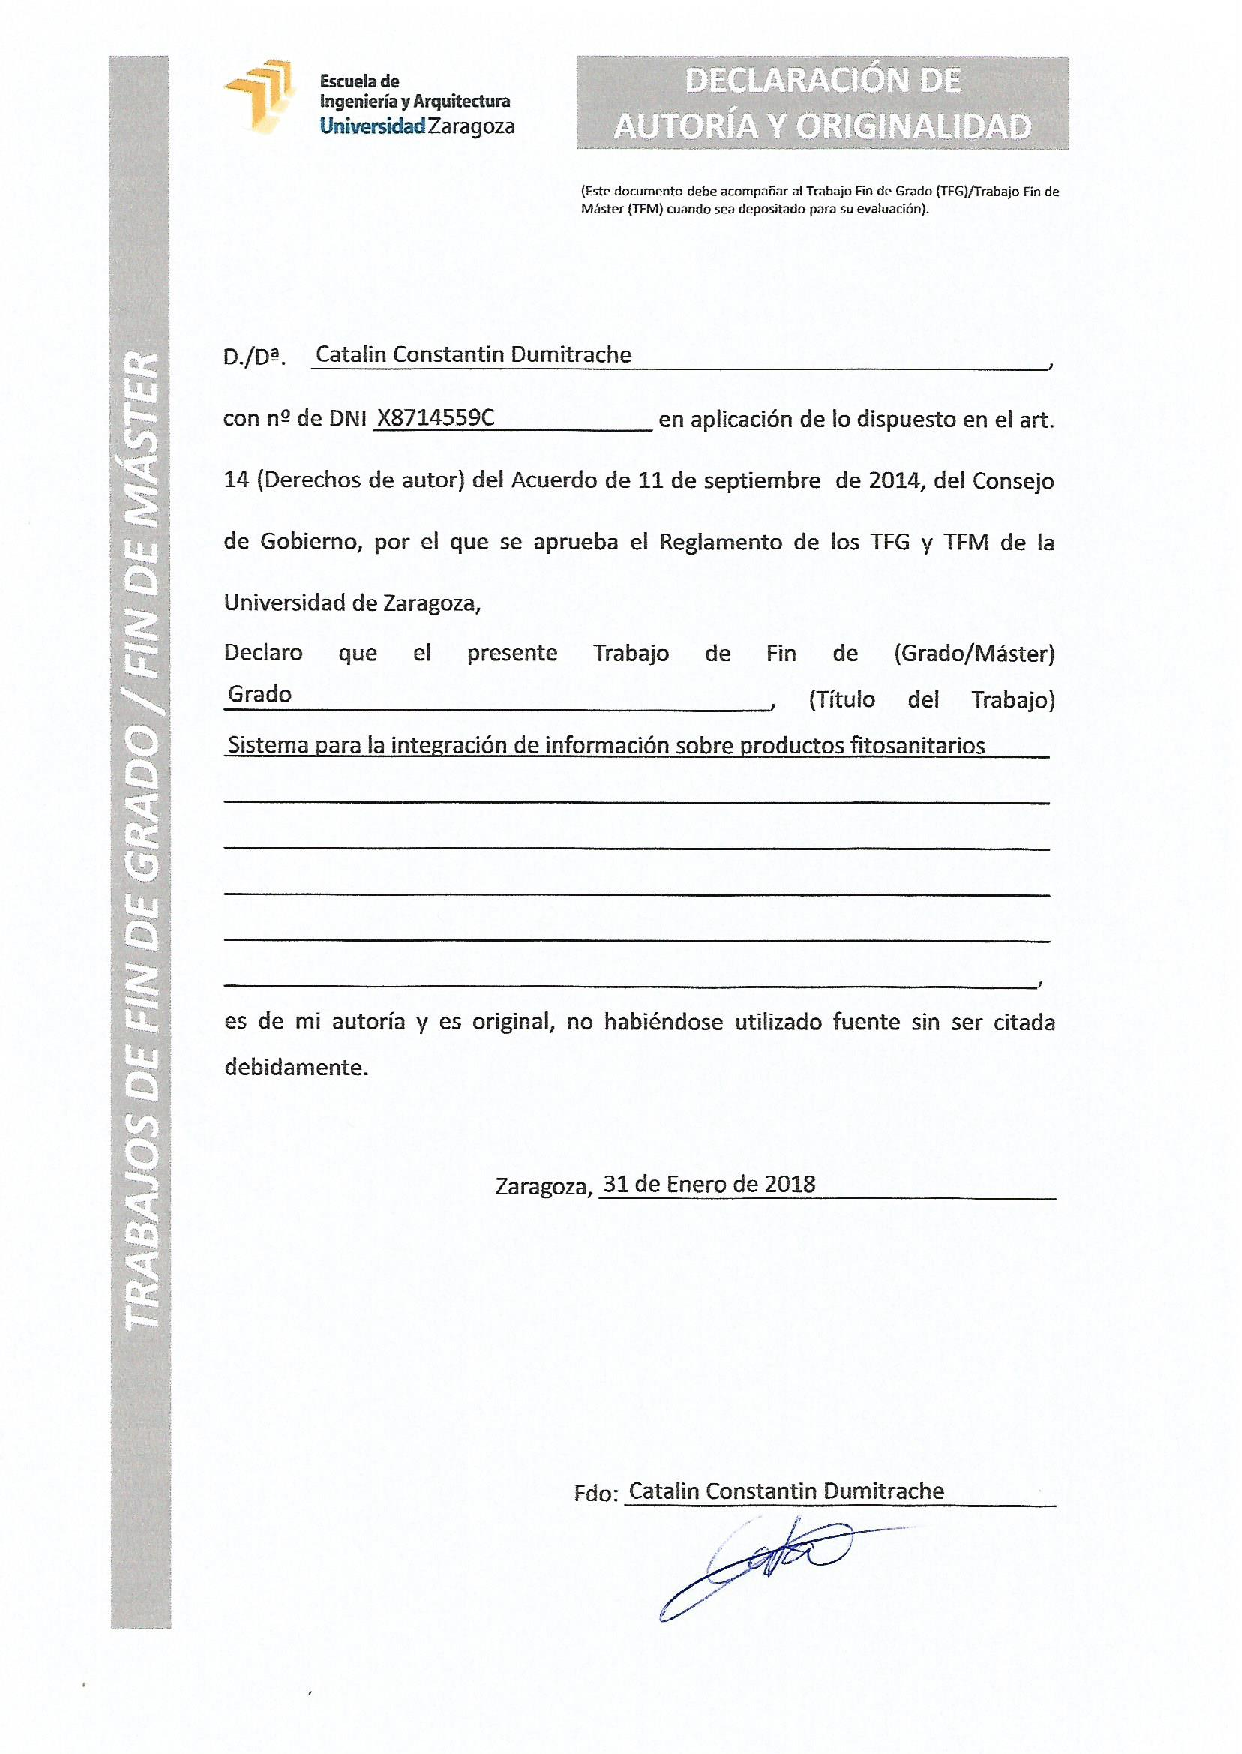
\includepdf[pagecommand={}]{Impreso}
\cleardoublepage


%%%%%%%%%%%%%%%%%%%%%%%%%%%%%%%%%%%%%%%%%%%%%%%%%%%%%%%%%%%%%%%%%%%%%%%%%%%%%%%%%%%
%		Resumen
%%%%%%%%%%%%%%%%%%%%%%%%%%%%%%%%%%%%%%%%%%%%%%%%%%%%%%%%%%%%%%%%%%%%%%%%%%%%%%%%%%%

\newpage

\begin{center}
{\Large \bfseries AGRADECIMIENTOS}
\vspace{2.5cm}
\end{center}


Agradezco a ... 
\newpage
\begin{center}

{\Large \bfseries RESUMEN EJECUTIVO}

\vspace{1.5cm}
\end{center}


Este proyecto se centra en presentar y demostrar un modelo de integración de información relativa a productos fitosanitarios y su aplicación en diferentes productos agrícolas provenientes de fuentes heterogéneas en un esquema único y escalable. \par
Para lograr esto, se han seleccionado diferentes fuentes de datos sobre productos fitosanitarios, presentes en distintos formatos y se han analizado varias tecnologías de integración para elegir el stack tecnológico que más se adecue al problema en cuestión. Dada la naturaleza del mismo, se puede englobar dentro de un panorama de programación y tecnologías \textit{Big Data}.
\par
Así pues, en este proyecto se han usado herramientas de almacenamiento elegidas bajo un criterio de escalabilidad futura y herramientas de procesado de datos bajo el criterio de proporcionar soporte al mayor abanico de fuentes heterogéneas posibles. El proyecto emplea una base de datos no relacional como sistema responsable del almacenamiento gracias a sus características de escalabilidad, en conjunto con una herramienta capaz de acceder a los datos almacenados a través de una aproximación relacional. Para el procesado de los datos se ha hecho uso de una herramienta que ofrece soporte al procesado de ficheros provenientes de diferentes fuentes, entre las que se encuentra la base de datos elegida, mencionada en este apartado.\par
Para demostrar la viabilidad del sistema, se ha desarrollado un prototipo funcional que recoge datos sobre productos fitosanitarios a nivel de España y Europa e integra la información de ambas fuentes, constituyendo un primer paso hacia ese modelo compartido donde varias fuentes heterogéneas concuerdan en un mismo esquema congruente. Los datos se pueden ver mediante una aplicación web desarrollada con un generador de proyectos ligero sobre \textit{Java} capaz de desplegar rápidamente una aplicación con una cuidada \textit{GUI}.  \\\par

\textbf{Palabras clave:} Integración, Big Data, Productos fitosanitarios, Procesado, Base de datos no relacional, Modelo único, Escalabilidad, Fuentes heterogéneas.

\newpage
% Quita los "Capítulo X" de cada capítulo. 
%\renewcommand{\chaptername}{}
%\renewcommand{\thechapter}{}

%\cleardoublepage
\renewcommand{\contentsname}{Tabla de contenidos}
\tableofcontents

%%%%%%%%%%%%%%%%%%%%%%%%%%%%%%%%%%%%%%%%%%%%%%%%%%%%%%%%%%%%%%%%%%%%%%%%%%%%%%%%%%%
%		Capítulos
%%%%%%%%%%%%%%%%%%%%%%%%%%%%%%%%%%%%%%%%%%%%%%%%%%%%%%%%%%%%%%%%%%%%%%%%%%%%%%%%%%%

\chapter{Introducción} \label{introduccion}
\pagenumbering{arabic}
Actualmente el proceso de consulta del uso y aplicación de los productos fitosanitarios sobre determinados productos resulta una tarea en ocasiones tediosa, sobre todo, cuando se trata de comprobar las especificaciones y regulaciones que imponen diferentes países en operaciones de importación o exportación de determinados productos agrícolas. Hoy en día, una persona que quiere comercializar estas sustancias debe tener en cuenta varios factores; en primer lugar, existen varios manuales extensos que recogen medidas de seguridad, buenas prácticas y pautas sobre la aplicación de los productos fitosanitarios. Dichos manuales se deben cumplir en todo momento [manual seguridad, aplicación fitosanitarios, buenas prácticas]. No solo eso, sino que por otra parte, las bases de datos o almacenes que recogen la información sobre productos fitosanitarios en muchas ocasiones no están bien gestionadas, son difíciles de encontrar, la información se presenta en formatos heterogéneos e incluso se puede encontrar desactualizada. Los avances conseguidos en este TFG pretenden reducir la complejidad de esa tarea de búsqueda de información acerca de productos fitosanitarios, facilitando a una persona el acceso a un esquema común con toda la información centralizada y actualizada.\par

El objetivo principal de este proyecto es \textbf{proponer y validar un proceso de recogida, transformación y presentación de la información sobre productos fitosanitarios con el resultado en forma de esquema compartido estandarizable} que pueda beneficiar tanto a agricultores como a instituciones nacionales o internacionales, \textbf{y facilitar la consulta de dicha información de manera más rápida, simple y accesible que los métodos actuales}. \par
Entre los retos planteados figuran:
\begin{itemize}
\item Desarrollar un sistema capaz de visualizar los datos ya integrados nutriéndose únicamente de las fuentes originales sin intervención de una persona en el proceso
\item La consistencia de los datos y su almacenamiento tanto en formato original como en su formato procesado e integrado en la versión final
\item El diseño de una solución escalable y actualizada en todo momento
\item La posibilidad de añadir características de trazabilidad y mantenimiento a la aplicación.
\end{itemize}

\section{Estructura del documento} \label{introduccion.estructura}
	
Este documento se presenta dividido en varios bloques conceptuales; el primero abarca los primeros tres apartados (Resumen ejecutivo, Introducción  y Definiciones) y se corresponde a una introducción al trabajo realizado. En él, se ofrece una visión completa y resumida del problema junto con su solución y se dan algunas definiciones técnicas de algunos de los términos empleados en esta memoria. El bloque de análisis abarca los apartados 4 y 5 (Phytoscheme y Análisis) y presentan el trabajo de análisis que se llevó a cabo, desde el estudio del entorno, hasta el análisis del stack tecnológico, pasando por el de riesgos y la captura de requisitos. El tercer bloque se corresponde a la solución desarrollada en sí; abarca los apartados 6 y 7 (Diseño e implementación) y se plasma el trabajo desde las fases tempranas del desarrollo de la solución hasta el momento de la finalización del software como solución tecnológica al problema.  Los últimos bloques se corresponden a los detalles de gestión del proyecto, a las conclusiones tanto del proyecto como del alumno a nivel personal y a los diferentes anexos recogidos durante toda la duración del TFG.


\chapter{Phytoscheme} \label{phytoscheme}
\section{Contexto y necesidades reales} \label{phytoscheme.contexto}
Los productos fitosanitarios son un elemento imprescindible en la producción agrícola, tanto en los sistemas convencionales de agricultura como en los sistemas de agricultura integrada o ecológica. Sin su existencia, muchos cultivos de las zonas de producción de mayor interés económico y social serían inviables hoy en día debido a los estragos potenciales de las diferentes clases de plagas.\par
No obstante, el uso de dichos productos fitosanitarios debe estar regulado ya que una aplicación indebida de los mismos puede tener otros efectos no deseables. Dichos efectos de ninguna manera deben suponer un peligro para la salud humana y tampoco riesgos inaceptables para el medio ambiente. \par
Por ello el Estado sólo aprueba la comercialización de aquellos productos fitosanitarios que sean útiles para combatir las plagas pero no impliquen otros riesgos colaterales. Para que un \gls{fito} pueda comercializarse debe estar inscrito necesariamente en el Registro Oficial de Productos Fitosanitarios - \textit{Página web del ministerio de agricultura y pesca, alimentación y medio ambiente de España} \cite{mapama}\par
Es, por tanto, necesario y casi obligatorio que la información del Registro de Productos Fitosanitarios llegue de manera precisa a todos los implicados en el área del uso de los productos fitosanitarios\par
La \textit{Directiva 2009/128/CE} \cite{directiva128} establece el marco de la actuación comunitaria para conseguir un uso sostenible de los productos fitosanitarios. Esta Directiva implica, por ejemplo, la obligación del registro del uso de productos fitosanitarios. Un ejemplo del desarrollo de esta Directiva es el \textit{Cuaderno de Explotación} \cite{cuadernoexplotacion}. Este cuaderno aglutina de manera ordenada y armonizada todos los elementos que deberán registrar los titulares de las explotaciones agrícolas, con el objetivo de facilitar el cumplimiento de la Directiva.\par
Actualmente, hay varias empresas que ofrecen aplicaciones (p. ej. \textit{aGROSLab} \cite{agroslab}, \textit{Agricolum} \cite{agricolum} o el \textit{Cuaderno de Campo Agronev} \cite{agronev}) que implementan el Cuaderno de Explotación. Un valor añadido que suelen incorporar estas aplicaciones es una base de datos con información acerca de los productos fitosanitarios autorizados. El problema al que se enfrentan estas empresas es que esta información no se publica de forma uniforme en toda la Unión Europea. Es decir, hay al menos un publicador por país miembro, la información publicada es heterogénea y los formatos normalmente son difícilmente accesibles. Además, a nivel Europeo, hay una \textit{base de datos de referencia} \cite{pesticidesdb} de las restricciones más o menos comunes en el uso de productos fitosanitarios. Dado que no hay un estándar de publicación establecido, una consecuencia adicional de esta situación es que es complicado verificar si un producto tratado con una serie de productos fitosanitarios en un país miembro puede ser exportado a otro, ya que la normativa fitosanitaria aplicable puede diferir.\par
En cuanto a la importación de productos desde un país miembro de la Unión Europea, el artículo 52 del \textit{Reglamento (CE) 11/07/2009} \cite{reglamento} se refiere a este trámite como comercio paralelo y se especifica que para poder llevarlo a cabo, el Estado Miembro donde se desee introducir deberá determinar que el producto fitosanitario es idéntico en composición a otro ya autorizado en su territorio al que se denominará “producto de referencia”. Para realizar el trámite, actualmente el proceso consta en rellenar la \textit{solicitud} del \gls{certificado} \cite{solicitud} (disponible en la página web del ministerio), entregarla a la Subdirección General de Higiene Vegetal y Forestal y esperar a que sea aprobada - \textit{Preguntas frecuentes Mapama} \cite{faqmapama} \par
Los principales problemas actuales de este proceso vienen por una parte en el lado del agricultor/empresa que solicita la importación puesto que no solo el tiempo de respuesta en ocasiones puede ser muy largo (de hasta de 45 días - Artículo 52, punto 2 del Reglamento (CE) 11/07/2009) sino que además, el agricultor o bien tiene poca información acerca de los productos permitidos en una importación/exportación o el acceso a dicha información es bastante tedioso y complicado. Por otra parte en el lado de la institución certificadora encargada de comprobar la solicitud el proceso no es del todo eficiente debido al hecho de tener que verificar manualmente si el producto cumple con los requisitos de composición del correspondiente producto en el país de importación/exportación. Estos problemas se pueden observar claramente en el siguiente diagrama, que muestra un flujo típico en un trámite de comercio paralelo entre un agricultor/empresa que quiere importar un producto a un determinado país, en este caso, España: 

\begin{figure}[H]
    \centering
    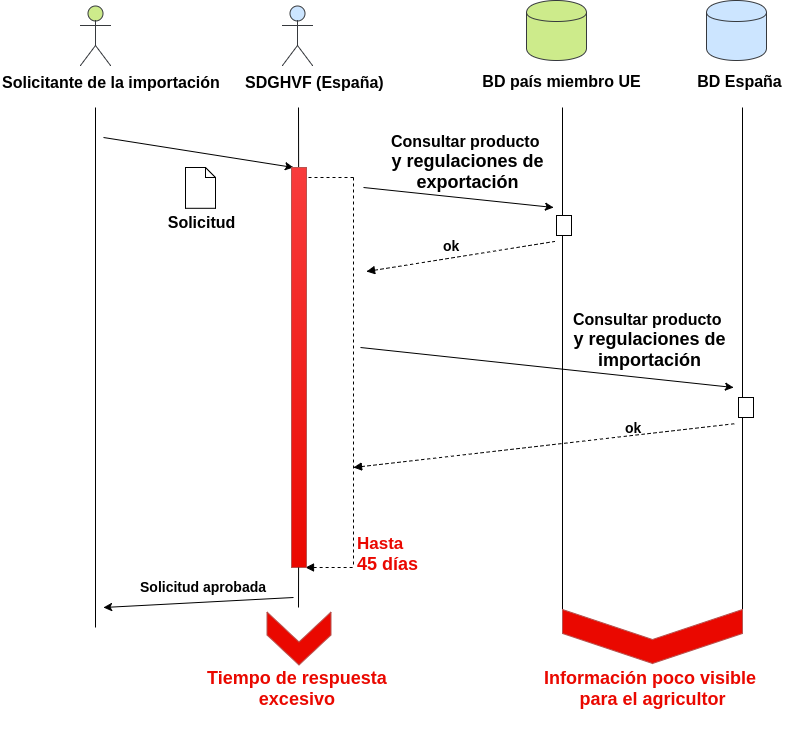
\includegraphics[width=1\textwidth,height=14cm]{Imagenes/Diagrama_de_flujo_proceso_actual_de_importacion_producto_fitosanitario}
    \caption{Diagrama de flujo del proceso actual de importación de un producto fitosanitario}
    \label{fig:flujo_actual_importacion}
\end{figure}
\par
*SGHVF = Subdirección General de Higiene Vegetal y Forestal\\\par
Es razonable desarrollar un sistema que provea un esquema único donde los datos estuvieran integrados y congruentes entre los diferentes países de la unión europea para facilitar un consumo posterior por las aplicaciones, e, incluso, directamente por los agricultores. 

\section{Motivación y objetivos} \label{phytoscheme.motivacion}
Habiendo visto el panorama descubierto en el apartado anterior, era evidente que se podían introducir mejoras al proceso actual que pueden beneficiar a las partes involucradas (tanto a agricultores y empresas como a las instituciones reguladoras). Con ese objetivo en mente, se propone desarrollar una aplicación prototipo que valide el proceso de integración de la información de diferentes países en un esquema único que recogiese los datos que de otra manera tendrían que ser recopilados manualmente, con largos tiempos de espera y con una incertidumbre por parte de los agricultores/empresas en lo que a datos sobre productos fitosanitarios respecta.\par 
El siguiente diagrama muestra el potencial proceso que tendría que seguir una persona interesada en realizar una importación y los problemas que sería capaz de solucionar el desarrollo de la aplicación planteada en este proyecto:

\begin{figure}[H]
    \centering
    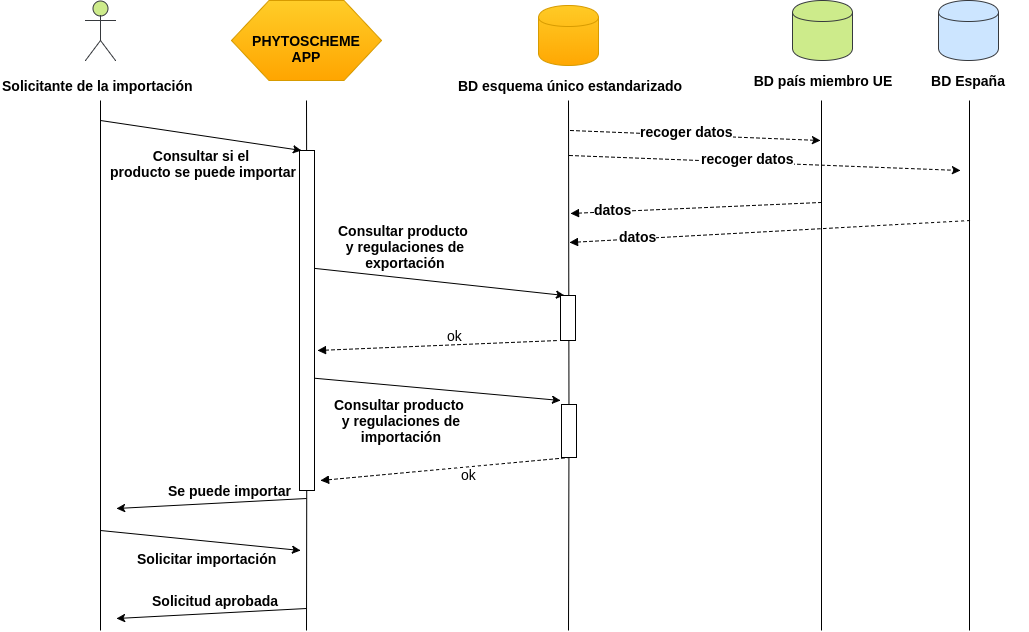
\includegraphics[width=1\textwidth,height=11cm]{Imagenes/Diagrama_de_flujo_proceso_potencial_de_importacion_producto_fitosanitario}
    \caption{Diagrama de flujo del potencial  proceso de importación de un producto fitosanitario}
    \label{fig:flujo_potencial_importacion}
\end{figure}
\par

Se puede apreciar que con este desarrollo se conseguiría no solo reducir los plazos de respuesta al agricultor/empresa sino también una mayor transparencia en la consulta de los datos, puesto que al estar integrados en un modelo único, el agricultor/empresa o los interesados podrían tener acceso a toda la información y consultar cualquier aspecto que de otra manera habría sido prácticamente inaccesible. No solo eso, sino que además, al conseguir un modelo potencialmente estandarizado, no haría falta del trabajo manual y tedioso de comprobación de los requisitos por parte de la Subdirección General de Higiene Forestal y Vegetal sino que sería el propio sistema el encargado de comprobar si la petición del solicitante cumple con la \textit{\gls{legisfito}} vigentede cada país. \par
Uno de los aspectos a tener en cuenta al comienzo del proyecto fue el hecho de que para que la solución se pudiera aplicar a un nivel real del problema, se necesitaba una gran capacidad de almacenamiento. Los datos deberían almacenarse periódicamente y además, potencialmente podrían provenir de multitud de fuentes, en diferentes formatos, con unos tamaños variables y constantes actualizaciones. Muchas fuentes equivalen a muchos datos, y muchos datos equivalen a la necesidad de un sistema de almacenamiento capaz de soportar toda esa carga. 
\par
Unido a esto, la elección de dicho sistema de almacenamiento suponía un punto crítico, puesto que no bastaría con cualquier base de datos sino que tendría que cumplir ciertas características como la posibilidad de guardar los datos en sus formatos originales, la necesidad de generar una jerarquía para su almacenamiento, o la posibilidad de integración con los trabajos de transformación y procesado de los datos. 
\par
Por ello, el proyecto tuvo como objetivo principal desarrollar una solución prototipo para demostrar la validez de los procesos y herramientas involucradas en la integración de varias fuentes heterogéneas de productos fitosanitarios en un modelo único.

\section{Restricciones} \label{phytoscheme.restricciones}
\par
Teniendo en cuenta que el proyecto actual es un TFG y no un proyecto comercial, se tienen que tomar en cálculo una serie de restricciones que vienen dadas tanto por la naturaleza del proyecto como por los partícipes del mismo. En primer lugar, siendo un TFG, debe realizarse una cantidad de esfuerzo equivalente a 12 ECTS.. Dado que el desarrollo realizado en este proyecto está enfocado a formar parte de un plan mucho mayor, donde el trabajo realizado se retomará y ampliará en futuros TFG, desde el principio se delimitaron aquellas características que se deseaban incluir en el proyecto y también aquellas que no corresponden a esta iteración.  Siendo una fase temprana de dicho plan maestro, a esta fase le correspondía la parte de validación del modelo, de las tecnologías empleadas y de la viabilidad del producto, no siendo primordial tener un producto final robusto sino demostrar que las tecnologías en su totalidad se complementaban y funcionaban acorde a lo esperado. 
\par
Otro factor restrictivo dada la naturaleza del proyecto es el hecho de que existe un director, que puede marcar las pautas de desarrollo, sugerir e imponer metodologías de trabajo o incluso herramientas del stack tecnológico que pueden suponer una ventaja o una desventaja en el desarrollo del proyecto. El alumno debe ser capaz de discutir estas tendencias con el director y razonar las decisiones que se tomen, en conjunto, y exponiendo sus puntos de vista con el objetivo de llegar a un acuerdo común. 

\section{Requisitos - Técnica \textit{\gls{moscow}}} \label{phytoscheme.requisitos}
\par 
Por imposición y recomendación del director del proyecto, el análisis y la captura de requisitos han estado desde el principio  regidos por el método \textit{\gls{moscow}}, una técnica de priorización de requisitos usada en la gestión de proyectos, análisis de negocio y desarrollo de software con objetivo de llegar a un acuerdo común con los \textit{stakeholders} (integrantes del proyecto) sobre la importancia que se debería dar a cada requisito. Esta técnica también es conocida bajo los nombres de \textit{priorización \gls{moscow}} o \textit{análisis \gls{moscow}}.
\par
La metodología \textit{\gls{moscow}} dicta cuatro categorías mediante las que se pueden priorizar los requisitos de un sistema o proyecto: 

\begin{enumerate}
\item \textbf{Debe tener:} Son aquellos requisitos críticos para que el trabajo realizado durante un periodo de tiempo determinado (en nuestro caso desde ahora hasta junio 2017) sea considerado un éxito (\textit{TFG} aprobado). Si uno de estos requisitos no se incluye, el proyecto debera ser considerado un fallo (no se puede presentar el \textit{TFG}). \textit{Debe tener} en \textit{\gls{moscow}} se refiere a \textit{MUST}, que puede ser considerado un acrónimo de \textit{Minimum Usable SubseT}. En ese sentido se puede entender como la unión de los requisitos del producto mínimo viable con los requisitos legales (p.ej. documentación en forma de memoria de \textit{TFG}, cumplimiento \textit{LOPD}, etc.) y de seguridad (en el sentido de robustez y calidad de la solución) obligatorios o acordados. Los requisitos del proyecto acordados para esta categoría han sido los siguientes: 
\begin{itemize}
\item Recolectar datos oficiales tanto de productos fitosanitarios autorizados de España como de las sustancias activas a nivel europeo. 
\item Almacenar la última versión de los datos en formato original y además mantener todas las versiones descargadas. 
\item Monitorizar y almacenar los procesos de recolección de los datos de entrada así como las rutas de su procesado.
\item Ofrecer la infraestructura y las herramientas de configuración necesarias para una expansión futura del proyecto. 
\item Implementar un modelo de aplicación consistente, ejemplificando el ciclo de vida típico de los datos desde su recogida hasta su presentación visual. 
\item Una memoria extensa y detallada. 
\end{itemize}

\item \textbf{Debería tener:} Son aquellos que son importantes pero no necesarios para ser realizados durante el periodo de tiempo determinado. Pueden posponerse para ser realizados en el siguiente periodo. Son vitales pero no obligatorios, si no se implementan la solución es viable pero es doloroso no hacerlo. En el caso de nuestro proyecto, dentro de esta categoría se han identificado los siguientes requisitos: 
\begin{itemize}
\item Mecanismo de control de esfuerzos.
\item Mecanismo de control de versiones.
\item Módulo de trazabilidad de los datos desde las fuentes originales hasta su visualización. 
\item Mecanismo de detección de errores e inconsistencias en los datos provenientes de diferentes fuentes. 
\end{itemize}


\item \textbf{Podría tener:} Son aquellos que comparados con los anteriores son los menos deseados o tienen menor impacto. Hay que tenerlos controlados ya que sólo se podrán entregar si se dan las mejores condiciones (por ejemplo, el proyecto va más rápido de los esperado). Si hay algún riesgo en la entrega del proyecto estos requisitos serían los primeros en ser descartados. A continuación se pueden ver los requisitos del proyecto que se han ubicados dentro de esta categoría:

\begin{itemize}
\item Genericidad en cuanto al soporte de integración de los datos de diferentes fuentes basado en un fichero de claves y valores. 
\item Soporte para la búsqueda de registros (datos) desde la interfaz web. 
\item Desarrollo dirigido por un paradigma de inversión de independencias para conseguir un control centralizado.
\end{itemize}

\item \textbf{No tendrá:} Son aquellos que no van a ser entregados durante el periodo considerado. Se mantienen en esta lista de alcance para clarificar el alcance de la solución. Esto evita que informalmente sean introducidos más tarde. El objetivo de esta categoría es ayudar a mantener el foco en una solución estricta. 


\begin{itemize}
\item Rediseño y desarrollo en el lado del \textit{Front-End}.
\item Desarrollo de tests adicionales en el proyecto de \textit{JHipster}
\item Integración de más de dos fuentes de datos heterogéneas. 
\end{itemize}


\end{enumerate}




\chapter{Análisis}
\section{Análisis del problema}
Como ya se ha aclarado varias veces a lo largo de este documento, actualmente hay una necesidad real en el mundo agrícola; la de disponer de la información sobre productos fitosanitarios de una manera centralizada, actualizada y de fácil acceso. Hoy en día esta necesidad se ha intentado abordar de varias maneras, y por ello hay disponibles varias aplicaciones que intentan apoyar al consumidor en las tareas agrícolas que involucran productos fitosanitarios. Algunos ejemplos son los productos que ofrecen empresas como aGROSLab, Cuaderno de Campo Agronev, o Agricolum. No obstante, estas aplicaciones se enfrentan al mismo problema; la inexistencia de una base de datos estandarizada cuya información sea congruente a través de los diferentes países de la Unión Europea. Por eso mismo, estas aplicaciones tienen que implementar, desarrollar y mantener ellas mismas las bases de datos que permitan acceder a la información deseada. Nuestra solución ofrecería un sistema dotado de una base de datos estandarizada, congruente en su información y completa, de código abierto y altamente escalable, por lo tanto todas las aplicaciones mencionadas arriba podrían convertirse en potenciales clientes consumidores de nuestro sistema, sustituyendo sus bases de datos por nuestra solución, con costes de integración mínimos.

\section{Modelo de negocio}
El modelo de negocio es el que se puede observar en la figura de la derecha. Se trata de una plantilla estándar para definir los aliados, las actividades y los recursos clave que intervienen en el proyecto, al igual que la propuesta de valor, la relación con los clientes, los canales de comunicación y los diferentes segmentos de clientes que tiene el proyecto. \par
Por otra parte también se pueden observar los costes que presenta el proyecto y también los ingresos o beneficios esperados tras su finalización por parte del alumno. \par
A continuación se explica cada uno de los apartados que incluye, en un orden que convenga más que el definido por la propia plantilla: 
\begin{itemize}
\item \textbf{Segmentos de clientes:} Aquí se mencionan los clientes a los que se distribuiría el resultado del producto, o a aquellos a los que sería dirigido. En este caso, por una parte existen tres tipos de clientes que recibirían el producto final (Agricultores que comercializan productos, Instituciones encargadas de validar la importación / exportación  de productos agrícolas, Importadores / Exportadores de productos agrícolas, pesqueros y alimentarios) que serían los que se beneficiarían directamente de los resultados del proyecto. Es a ellos a quien va dirigida la aplicación puesto que haría más simple el proceso de comprobación de los requisitos fitosanitarios sobre los productos agrícolas / pesqueros / alimentarios. Por otra parte están los clientes a los que va dirigido el proyecto dentro de la Universidad de Zaragoza. Estos son el tribunal de defensa del proyecto y el director del proyecto, que estará en constante contacto con el alumno. 
\item \textbf{Propuesta de valor:}Se mencionan qué cosas aporta el proyecto a los clientes mencionados en el apartado anterior. Estas son:
\begin{itemize}
\item Análisis de las técnicas actuales involucradas en la comprobación de aplicación de los productos fitosanitarios a un determinado producto - puesto que para determinar qué problemas se pretenden solucionar, primero se debe entender bien el proceso actual.
\item Diseño de una solución de integración que recoge datos sobre productos fitosanitarios de varios países y los integra en un esquema único - que pretende solucionar algunos de los problemas actuales.
\item Desarrollo de una aplicación que muestre los resultados de manera gráfica - para demostrar los resultados tanto al tribunal como a los potenciales clientes.
\item Redacción de un documento explicativo del proceso anterior - la memoria, que servirá para que el tribunal comprenda la dedicación y el esfuerzo invertido en el proyecto y los avances y logros obtenidos.
\end{itemize}
\item \textbf{Relación con los clientes:} Si bien es cierto que habrá una relación con los clientes finales de la aplicación, como ese aspecto no le corresponde al alumno sino a la Universidad de Zaragoza, no se mencionan dicho tipo de relaciones en este apartado. No obstante, si se mencionan los dos tipos de relaciones que tienen que ver con los resultados que el alumno debe presentar ante el tribunal de defensa, es decir, la memoria del proyecto y una breve presentación formal donde se expondrán los puntos de interés del desarrollo del proyecto. De igual manera, en la relación del alumno con el director del proyecto, periódica y frecuentemente habrá revisiones del trabajo realizado y se hará un seguimiento continuo para observar la evolución del mismo.
\item \textbf{Aliados clave:} Dada la naturaleza del proyecto, los principales aliados son la Universidad de Zaragoza y el director del proyecto, en este caso Javier López Pellicer.
\item \textbf{Actividades clave} que se han realizado en el proyecto:
\begin{itemize}
\item Desarrollo prototipo de integración
\item Recogida y procesado de los datos desde sus formatos originales
\item Presentación de los datos
\end{itemize}
\item \textbf{Recursos clave} con los que ha contado el alumno para desarrollar el proyecto 
\begin{itemize}
\item Equipo de trabajo (portátil propio)
\item Laboratorio de investigación - provisto por el director del proyecto, ubicado en el laboratorio L2.09 del edificio Ada Byron, en la Escuela de Ingeniería y Arquitectura de Zaragoza.
\item Herramientas open source - Todo el stack tecnológico, debido a un presupuesto nulo ha tenido que ser gratuito.
\item 300 horas contables de trabajo, las recomendadas para proyectos de este tipo.
\end{itemize}
\item \textbf{Estructura de costes:} Costes económicos o temporales que el alumno ha invertido en el proyecto:
\begin{itemize}
\item Primera matrícula del proyecto: 259,92
\item Segunda matrícula del proyecto: 408,96
\item Transporte mediante bus: Bono bus 90 días x 3 = 104,90 x 3 = 314,70
\item 300 horas invertidas en el trabajo
\begin{itemize}
\item TOTAL: 983,58 más las 300h de trabajo
\end{itemize}
\end{itemize}
\item \textbf{Estructura de ingresos:} Ingresos o partes de las que el alumno se beneficiaría tras la realización de este proyecto:
\begin{itemize}
\item Requisito de tener el proyecto finalizado - Por normativa cualquier estudiante matriculado en el Grado en Ingeniería Informática debe realizar y aprobar el trabajo de fin de grado.
\item Potencialmente el título universitario - Gracias al hecho de aprobar el proyecto, al encontrarse en una situación en la que al alumno lo único que le resta para acabar el grado es la realización del proyecto, posteriormente a su consecución podría obtener el título universitario. 
\end{itemize}
\end{itemize}

\section{Contexto tecnológico}
Dado que se trata de un escenario caracterizado por la heterogeneidad en contenidos y formatos de los datos, la necesidad de su procesamiento y de una escalabilidad futura, el proyecto está situado en un círculo de tecnologías Big Data, que presenta los siguientes retos:
\begin{itemize}
\item \textbf{Datos.} La información sobre los productos fitosanitarios no está habitualmente disponible en un formato estructurado. Es decir, la solución debe poder trabajar con datos en formatos no estructurados y ser capaz de procesarlos, idealmente convirtiéndolos a un formato relacional.
\item \textbf{Esquema.} No existe un esquema de referencia compartido para integrar la información de productos fitosanitarios de diferentes países, pudiendo darse el caso de la existencia de varios esquemas distintos en función del caso de uso. Es decir, la solución debe poder reconfigurar el esquema de integración con facilidad.
\item \textbf{Procesado.} Derivado del reto anterior, los datos no se pueden procesar y almacenar directamente en el esquema de integración sino que  deben guardarse en el formato original y ser procesados bajo demanda teniendo en cuenta las características específicas de cada fuente.
\item \textbf{Almacenamiento.} No se dispone de un presupuesto para invertir en un gran sistema de almacenamiento que permita almacenar los datos en formato original. Por ello, toda solución deberá ser de código abierto y poder ejecutarse sobre hardware de bajo coste.
Presentación de los datos. Es necesario desarrollar una interfaz visual para presentar los datos una vez integrados en un modelo único. 
\item  \textbf{Agilidad.} La solución debe poder evolucionar con facilidad. Cualquier desarrollador que utilice la solución debe poder reconfigurar rápidamente el esquema común y los servicios que exponen dicho esquema para su uso.
\item \textbf{Plazos.} Las limitaciones temporales y la priorización de tareas son influyentes en la elección del stack tecnológico, aunque en menor medida que los puntos anteriores. 
\end{itemize}

\section{Glosario del Stack Tecnológico}
Habiendo mencionado los factores anteriores, a continuación se presentan las tecnologías a las que se va a hacer referencia en el siguiente apartado con el objetivo de familiarizar al lector con las herramientas utilizadas:
\begin{itemize}
\item \textbf{\textit{Hadoop}.} \cite{hadoop} La librería software Apache Hadoop es un framework que permite el procesamiento distribuido de múltiples conjuntos de datos a través de clusters de ordenadores mediante modelos de programación sencillos. Está diseñado para escalar desde servidores únicos hasta miles de máquinas, donde cada una ofrece computación y almacenamiento local. Más que depender del hardware para prestar una alta disponibilidad, la librería en sí está diseñada para detectar y gestionar fallos en la capa de aplicación y así permitir una alta disponibilidad a pesar de que los equipos individuales fallen. 
\item \textbf{\textit{Hive}.} \cite{hive}  El software de data warehouse Apache Hive facilita la lectura, escritura y gestión de grandes conjuntos de datos residentes en almacenes distribuidos de datos mediante SQL. La estructura de datos puede ser proyectada sobre los datos que ya existen en almacenamiento. Apache Hive provee una herramienta de línea de comandos y un driver JDBC para que los usuarios se puedan conectar a Hive. 
\item \textbf{\textit{Sqoop}.} \cite{sqoop} Apache Sqoop es una herramienta diseñada para transferir bloques de datos entre Apache Hadoop y almacenes de datos estructurados como las bases de datos relacionales.
\item \textbf{\textit{JHipster}.} \cite{jhipster} JHipster es una plataforma de desarrollo para generar, desarrollar y lanzar aplicaciones con tecnología Spring Boot, AngularJS y Spring microservices. 
\item \textbf{\textit{Spring Framework}.} \cite{springframework} El framework Spring provee un modelo de programación y configuración sencillo para aplicaciones Java. Un punto clave de Spring es el soporte infraestructural a nivel de aplicación. 
\item \textbf{\textit{Spring Boot}.} \cite{springboot} Spring Boot es un framework ligero que tiene la intención de simplificar el proceso de configuración de una aplicación hecha con Spring. 
\item \textbf{\textit{AngularJS}.} \cite{angularjs} AngularJS es un framework de JavaScript de código abierto, mantenido por Google, que se utiliza para crear y mantener aplicaciones web de una sola página. Su objetivo es aumentar las aplicaciones basadas en navegador con capacidad de Modelo Vista Controlador (MVC), en un esfuerzo para hacer que el desarrollo y las pruebas sean más fáciles.
\item \textbf{\textit{Talend}.} \cite{talend} Talend es un software open-source de integración, procesado y transformación de datos. Permite trabajar con paradigmas Big Data y ofrece una interfaz gráfica para diseñar y programar cómodamente procesos ETL. 
\end{itemize}

\section{Elección del Stack Tecnológico}
Debido a los factores mencionados en el apartado anterior, el stack tecnológico se vio restringido a las herramientas mencionadas anteriormente; tal como se ha dicho, la solución necesitaba almacenar la información en crudo hasta el momento de su procesamiento y es por ello que una aproximación relacional habría sido inviable. Por lo tanto, viendo las diferentes opciones noSQL disponibles (MongoDB, Cassandra, DynamoDB, HBase, etc) y por recomendación del director del proyecto, la elección más clara fue elegir Hadoop como sistema de almacenamiento. Hadoop es una gran herramienta para el escalado de aplicaciones y lo utilizan grandes empresas para Big Data. Se adapta perfectamente a las necesidades de este proyecto y el software es gratuito. Además, hay una gran comunidad de personas capaces de ayudar con cualquier proyecto y la documentación disponible es lo suficientemente extensa como para salir de cualquier situación problemática. \par
No obstante, Hadoop por sí mismo no era capaz de solucionar todos los problemas del proyecto; Hadoop es capaz de almacenar los datos y, si bien es cierto que las operaciones de mapreduce permiten transformar dichos datos, dada la necesidad del desarrollo ágil del proyecto, lo mejor fue disponer de algún mecanismo más sencillo para el procesado de los mismos. Por ello, se decidió emplear Hive como herramienta de traducción de los datos almacenados en Hadoop, tanto en crudo como procesados, a una estructura relacional, sobre la que se podían hacer preguntas SQL. \par
El otro reto planteado fue la presentación de los datos integrados mediante una interfaz web, lo que vendría siendo el lado del cliente de la solución. Indudablemente hay casi infinidad de posibilidades para el desarrollo de esta parte. No obstante, realmente la parte de visualización no fue una parte crítica del proyecto, ni el objetivo del mismo. Es por ello que se adoptó una postura de desarrollo rápido del lado del cliente. JHipster (generador de aplicaciones sobre Spring) resultó la herramienta indicada, puesto que facilmente, en unos cuantos pasos era capaz de generar una aplicación sobre un esquema de base de datos (en este caso MySQL) y con una interfaz gráfica cuidada que satisfacía las necesidades del proyecto. No obstante, para poder conectar la base de datos de Hadoop con la base de datos MySQL necesaria para JHipster, el paso intermedio fue conectar Hadoop con Hive y realizar operaciones ETL de Hive a JHipster mediante Sqoop, una herramienta de transformación y carga de datos entre distintas bases de datos.\par
Teniendo en cuenta que los anteriores puntos constituyen el core tecnológico del proyecto, conforme se avanzaba se veía que no eran suficientes para conseguir los resultados deseados. Se tuvieron que emplear otras herramientas adicionales para diferentes tareas como el procesado de los datos previo a su exposición en Hive pero posterior a su almacenamiento en Hadoop, o la traducción de los datos y estructuras de Hive a la base de datos que emplea JHipster. Las elegidas fueron Talend Big Data (herramienta de procesado de ficheros capaz de conectarse a Hadoop,  extraer la información contenida en sus nodos, procesarla y volver a guardarla con los cambios efectuados, tal como se le indique) y Sqoop (herramienta diseñada para transferir bloques de datos entre Apache Hadoop o Hive y almacenes de datos estructurados como las bases de datos relacionales). 

\section{Análisis de riesgos}
En la fase inicial del proyecto se abordó el proceso de gestión de riesgos, para determinar los diferentes riesgos que podrían afectar a un proyecto de esta envergadura. Dicho proceso consta de varios pasos que en conjunto permiten tener una visión clara de aquello que puede entorpecer, frenar o incluso imposibilitar la finalización del proyecto. A continuación se listan dichos pasos y se presentan las conclusiones principales extraídas de cada una de ellas, dejando para los anexos la versión completa donde se puede apreciar detalladamente en cada paso todos los riesgos considerados con sus correspondientes valoraciones: 
\begin{enumerate}
\item En primer lugar, la identificación de riesgos permite determinar la lista de riesgos capaces de romper la planificación del proyecto. Durante esta fase se estudió qué factores podrían influenciar, en mayor o menor medida el flujo de trabajo normal del proyecto. Se agruparon en diferentes categorías para delimitar las zonas a las que afectaría cada riesgo. Así pues, aparecen 31 riesgos divididos en 4 clases:
\begin{enumerate}
\item Riesgos globales (referentes a todo el proyecto)
\item Riesgos tecnológicos (referentes a los aspectos más técnicos y tecnológicos del proyecto)
\item Riesgos de alcance (referentes al tamaño y alcance de la solución)
\item Riesgos de entorno de desarrollo (referentes tanto a la gestión como a las diferentes partes del entorno del desarrollador)
\end{enumerate}
\item El análisis de riesgo ofrece una medición de la probabilidad y el impacto de cada riesgo. Maneja tres valores que determinan la gravedad de un riesgo: 
\begin{enumerate}
\item la probabilidad con la que se puede dar un riesgo (rango entre 1 y 3, donde 1 es baja probabilidad y 3 es alta probabilidad)
\item el impacto que tendría en el resultado final un riesgo (rango entre 1 y 3, donde 1 es bajo impacto y 3 es alto impacto)
\item la aceptación del riesgo, una medida delimitadora que define aquellos riesgos que son considerados aceptables y aquellos ante los que se deben tomar medidas. Para esta medida se ha establecido un criterio de aceptación de 4. Cualquier riesgo cuyo valor sea menor que 4 se considera aceptable y por tanto un riesgo poco reseñable, mientras que aquellos que se encuentran por encima de 4 se consideran reseñables y se debe proceder a su tratamiento. 
\end{enumerate}
El cálculo de la gravedad del riesgo y su aceptación se realiza de la siguiente manera: se multiplica la probabilidad por el impacto, y si dicho valor excede el límite del criterio de aceptación, el riesgo se considera reseñable. En esta fase se detectaron un total de 6 riesgos reseñables, que se presentan en el siguiente punto.
\item La priorización de riesgos, fase donde se puede ver la lista de todos los riesgos anteriores ordenados por su gravedad. No obstante, a continuación se mencionan aquellos que han tenido un factor de gravedad superior a 4, límite del criterio de aceptación: 
\begin{enumerate}
\item RG\_1. Riesgo global “Plazos”. Tiene que ver con el hecho de no acabar el proyecto dentro de los plazos establecidos para su defensa. Hay 2 fechas recomendables para su defensa, la primera en Junio de 2017 y la segunda en Septiembre de 2017. No obstante, se dispone de otra oportunidad en Diciembre de 2017, aunque sería la menos recomendable dado que supondría el retraso de la defensa y con ello la dificultad del estudiante de realizar otras actividades mientras tanto. A partir de Diciembre, la consecuencia sería volver a matricularse en el proyecto y aportar las tasas de la matrícula por segunda vez.
\item RT\_2. Riesgo de tecnologías “Software no probado”. Tiene que ver con la probabilidad de usar en el proyecto software que previamente no ha sido probado y pueda fallar. Obtuvo una valoración de gravedad de 6/6 puesto que si bien es cierto que todas las tecnologías han sido probadas individualmente y se sabe que funcionan bien, el proceso en su conjunto no ha sido probado. No se sabe si es viable o no.  
\item RT\_6. Riesgo de tecnologías “Inalcanzable”. Relacionado con el hecho de que el proyecto puede tener como conclusión un resultado negativo; Al tratarse de un trabajo de investigación, el resultado puede ser que no se ha logrado la integración deseada.
\item RA\_1. Riesgo de alcance “Tamaño estimado”. Tiene que ver con el hecho de que el proyecto resulte mucho más grande de lo estimado inicialmente, y por diferentes circunstancias no se llegue a finalizar.
\item RA\_6. Riesgo de alcance “Número de cambios”. Otro riesgo es el hecho de que los requisitos cambien constantemente, bien porque los clientes lo solicitan bien porque las propias tecnologías lo imponen. 
\item RE\_9. Riesgo de entorno de desarrollo “Formación”. Este riesgo trata con el hecho de que el alumno disponga de la formación necesaria y suficiente para lograr los objetivos propuestos.
\end{enumerate}
\item Finalmente, la planificación de la gestión de riesgos, relativa al plan para tratar cada riesgo significativo.\\
En este apartado se recogieron los seis riesgos anteriores y se propuso para cada uno una solución mitigadora: 
\begin{enumerate}
\item RG\_1: Plazos - Como medida mitigante, el alumno deberá dedicar un horario de jornada completa a la realización del proyecto durante el verano del año 2017. 
\item RT\_2: Software no probado - La contrapartida y defensa de este riesgo es desarrollar o experimentar primero con una prueba de concepto para validar que las tecnologías en su conjunto funcionen correctamente. 
\item RT\_6: Inalcanzable - La mitigación este riesgo está ligada al anterior. Por lo tanto, primero se hará una prueba de concepto para demostrar si las tecnologías empleadas se pueden usar en conjunto.
\item RA\_1: Tamaño estimado - La solución desde un principio debe definir bien el alcance y determinar aquellas cosas que formarán parte de la solución y aquellas que no lo harán. 
\item RA\_6: Número de cambios - El alumno y el profesor deben acordar al principio unos requisitos fijos que no podrán ser modificables, en conjunto con el hecho de definir claramente el alcance de la solución.
\item RE\_9: Formación - Para mitigar este riesgo, el alumno debe estar en constante aprendizaje, utilizando los manuales y tutoriales de las diferentes herramientas de las que va a hacer uso durante el proyecto. Además, el alumno tendrá a su disposición al director del proyecto para consultar dudas y a los diferentes foros tecnológicos de Internet. 
\end{enumerate}
\end{enumerate}

\section{Captura de requisitos}
En una fase temprana del proyecto se realizó un análisis amplio y genérico del problema en conjunto con el director del proyecto. Se observaron y entendieron los retos a los que se enfrenta y se definieron los objetivos que se pretendía conseguir y por lo tanto los requisitos que se debían cumplir. A continuación se recogen en una tabla los requisitos, tanto funcionales como no funcionales divididos en sistema y proyecto, siendo los de sistema los referentes al propio producto tecnológico en sí, y los de proyecto los referentes a la gestión del mismo: \par
\begin{table}[!h]
\centering
\bgroup
\def\arraystretch{1.3}
\begin{tabular}{l p{13cm}}
\toprule
\textbf{Nombre} & \textbf{Descripción} \\
 \midrule
RFS\_1 & 
El sistema deberá recolectar los datos oficiales tanto de productos fitosanitarios como de pesticidas.
 \\
RFS\_2 & 
El sistema deberá almacenar la última versión de los datos recolectados en el RF\_1 en su formato original y además mantener todas las versiones del documento. 
 \\
RFS\_3 & 
El sistema deberá monitorizar, almacenar y mostrar los procesos de recolección de los datos de entrada, así como las rutas de su procesado. 
 \\
RFS\_4 & 
El sistema deberá ofrecer la infraestructura y herramientas de configuración necesarias para que futuros desarrolladores puedan integrar otras fuentes de datos de manera rápida y eficiente. 
 \\
RFS\_5 & 
El sistema deberá implementar un modelo de aplicación consistente, ejemplificando un ciclo de vida típico de los datos, desde su recogida, su procesamiento, su posterior integración en un modelo más completo y su presentación en un Front-End de ejemplo.
 \\
\bottomrule
\end{tabular}
\egroup
\caption{Requisitos Funcionales del Sistema}
\label{tab:req_func_sist}
\end{table}
\begin{table}[!h]
\centering
\bgroup
\def\arraystretch{1.3}
\begin{tabular}{l p{13cm}}
\toprule
\textbf{Nombre} & \textbf{Descripción} \\
 \midrule
RNFS\_1 & 
Los información de los productos fitosanitarios deberá ser recogida de portales como mapama y los datos sobre los pesticidas de la base de datos europea.
 \\
RNFS\_2 & 
Se hará uso de algún tipo de crawler web para la descarga periódica de los datos sobre fitos y pesticidas.
 \\
RNFS\_3 & 
Como sistema de almacenamiento de los datos recogidos sobre fitos y pesticidas se usará Hadoop.
 \\
RNFS\_4 & 
Para monitorizar, almacenar y mostrar los procesos de recolección de los datos de entrada se usará Talend Big Data. 
 \\
RNFS\_5 & 
Para conseguir unos desarrollos posteriores más ágiles se hará uso de la herramienta HIVE, que permite una aproximación relacional directamente sobre Hadoop.
 \\
RNFS\_6 & 
La presentación de los datos en su formato final se hará mediante una aplicación con GUI, desarrollada mediante la herramienta JHipster.
 \\
\bottomrule
\end{tabular}
\egroup
\caption{Requisitos No Funcionales del Sistema}
\label{tab:req_no_func_sist}
\end{table}
\begin{table}[!h]
\centering
\bgroup
\def\arraystretch{1.3}
\begin{tabular}{l p{13cm}}
\toprule
\textbf{Nombre} & \textbf{Descripción} \\
 \midrule
RFP\_1 & 
El proyecto deberá incluir una memoria en la que se documentan todos los pasos y procesos involucrados en su construcción.
 \\
RFP\_2 & 
Se deberá mantener constancia del esfuerzo dedicado durante el proyecto.
 \\
RFP\_3 &
El proyecto deberá mantener un control de versiones actualizado en todo momento. 
 \\
\bottomrule
\end{tabular}
\egroup
\caption{Requisitos Funcionales del Proyecto}
\label{tab:req_func_proy}
\end{table}












 



















\chapter{Diseño}  \label{disenyo}

Este capítulo abarca aquellos aspectos considerados durante la fase del diseño de la aplicación, desde sus versiones primitivas (diseño conceptual) hasta el diseño final de la aplicación, pasándo por los diferentes diagramas arquitecturales que muestran el sistema desde diferentes puntos de vista. Además, al final se hará una retrospectiva sobre aquellas restricciones que han afectado el curso del desarrollo de las diferentes soluciones desde el punto de vista del diseño. 


\section{Diseño conceptual} \label{disenyo.conceptual}
Con el análisis finalizado y teniéndo en cuenta los requisitos, se llegó a la conclusión de que los desarrollos realizados a lo largo de la duración de este proyecto no serían más que el comienzo para algo mucho más grande; se debía ofrecer tanto la infraestructura necesaria como el soporte para que la solución pudiera escalar y ser expandida mediante el trabajo de futuros desarrolladores. 


\par 
El diseño conceptual del sistema se presenta a continuación a una escala abstracta y de alto nivel. Básicamente, el proyecto hará uso de numerosas fuentes de información, en este caso sobre productos fitosanitarios y sus derivados. Dicha información deberá ser recogida de manera periódica y almacenada en algún sistema de persistencia tal como proviene de sus fuentes, es decir, en una versión \textit{en crudo}. Una vez almacenada en su versión original, los datos pasarán a una siguiente fase en la que serán procesados bien para extraer la información relevante o de interés para el proyecto bien para añadir datos útiles como información de trazabilidad, todo esto con el objetivo en mente de conseguir ese esquema unificado. Una vez procesados, los datos se almacenarán en otro sistema de persistencia, o incluso en el mismo de antes, si es posible. En este punto habría dos opciones; o que los datos ya estuvieran integrados en un único modelo, o que estuvieran individualmente separados en el almacén anterior. En este segundo caso, los datos deberían ser unificados para conseguir ese esquema único y posteriormente poder ser visualizados, ya sea mediante un navegador con una aplicación web, o mediante otro método de visualización. En el diagrama de la figura \ref{fig:disenyoconceptual} se puede observar el diseño conceptual descrito anteriormente de manera gráfica. 

\begin{figure}[H]
    \centering
    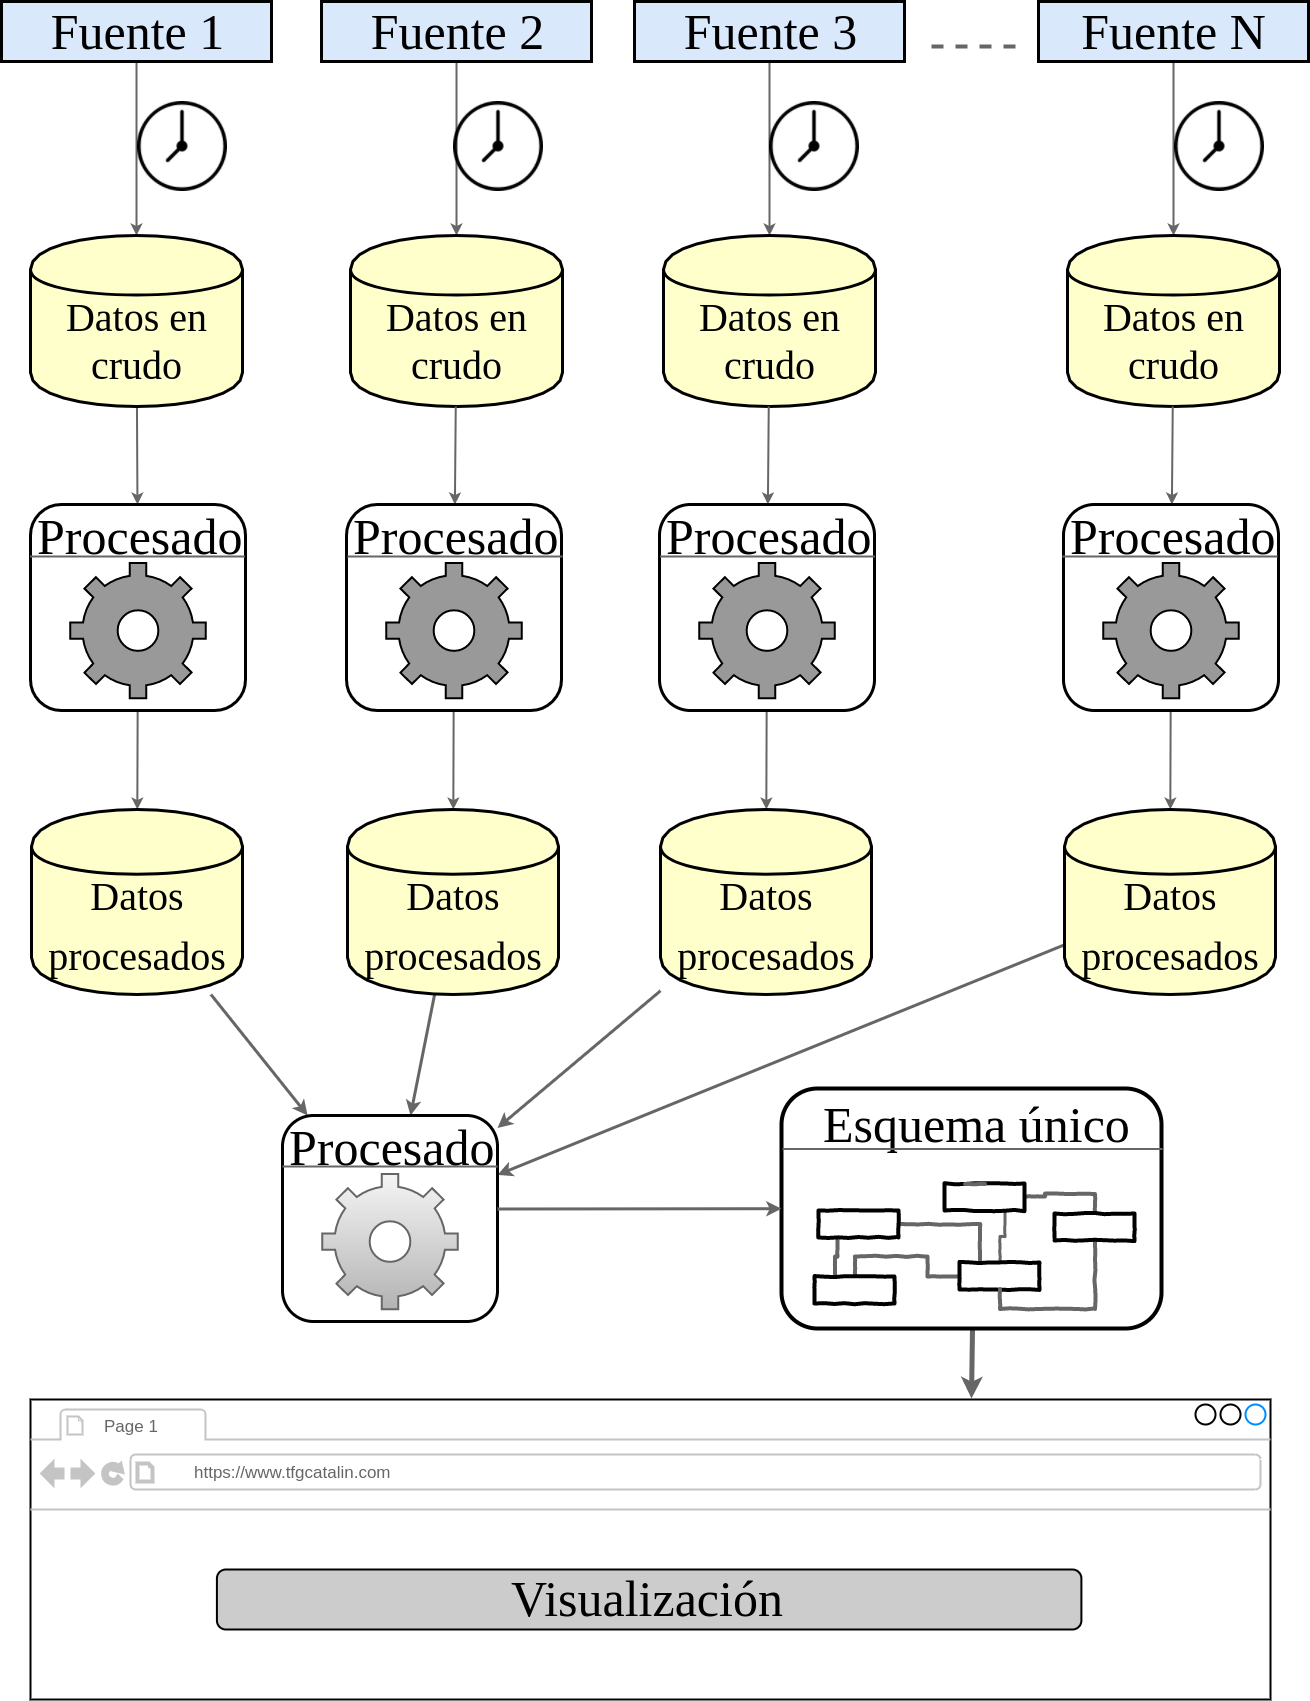
\includegraphics[width=1\textwidth,height=15cm,keepaspectratio]{Imagenes/disenyoconceptual}
    \caption{Diseño conceptual de la solución}
    \label{fig:disenyoconceptual}
\end{figure}




\section{Diseño final} \label{disenyo.final}



En el apartado anterior se ofreció una visión de alto nivel del diseño de la solución, sin hablar de herramientas ni de tecnologías concretas. En este apartado se va a profundizar en el diseño y se va a explicar en detalle la manera en que los datos pasan a través de las diferentes herramientas dentro del sistema, desde la descarga de los datos desde sus fuentes hasta su visualización en pantalla, pasándo por las diferentes etapas de procesado y almacenamiento. 
\par


En el diagrama de la figura \ref{fig:disenyofinal} se puede observar un mapeo casi directo entre los elementos del diseño final y los del diseño conceptual de la figura \ref{fig:disenyoconceptual}. Se puede observar que el diseño final incluye a \textit{Talend Big Data} como responsable tanto de los procesos que descargan y almacenan los \textit{datos en crudo} como de los que posteriormente procesan y almacenan los datos como \textit{datos procesados}. En cuanto al sistema de almacenamiento, que guardará tanto los datos originales como los modificados se utilizará \textit{Apache Hadoop} para los \textit{datos en crudo} y \textit{Apache Hive} dentro de \textit{Apache Hadoop} para los \textit{datos procesados}. Una vez los datos estén transformados y almacenados corréctamente, se usará \textit{Apache Sqoop} para transferirlos a ese esquema único que se persigue como objetivo, y que estará almacenado dentro de una base de datos \textit{MySQL}. Para que este último paso sea posible, debe ser el propio \textit{Talend} quien prepare los datos para ser integrados directamente en el esquema unificado. \textit{JHipster} tendrá una conexión directa a la base de datos \textit{MySQL} y gracias a ello será capaz de leer los datos y mostrarlos en pantalla con su propia interfaz web. 
\begin{figure}[H]
    \centering
    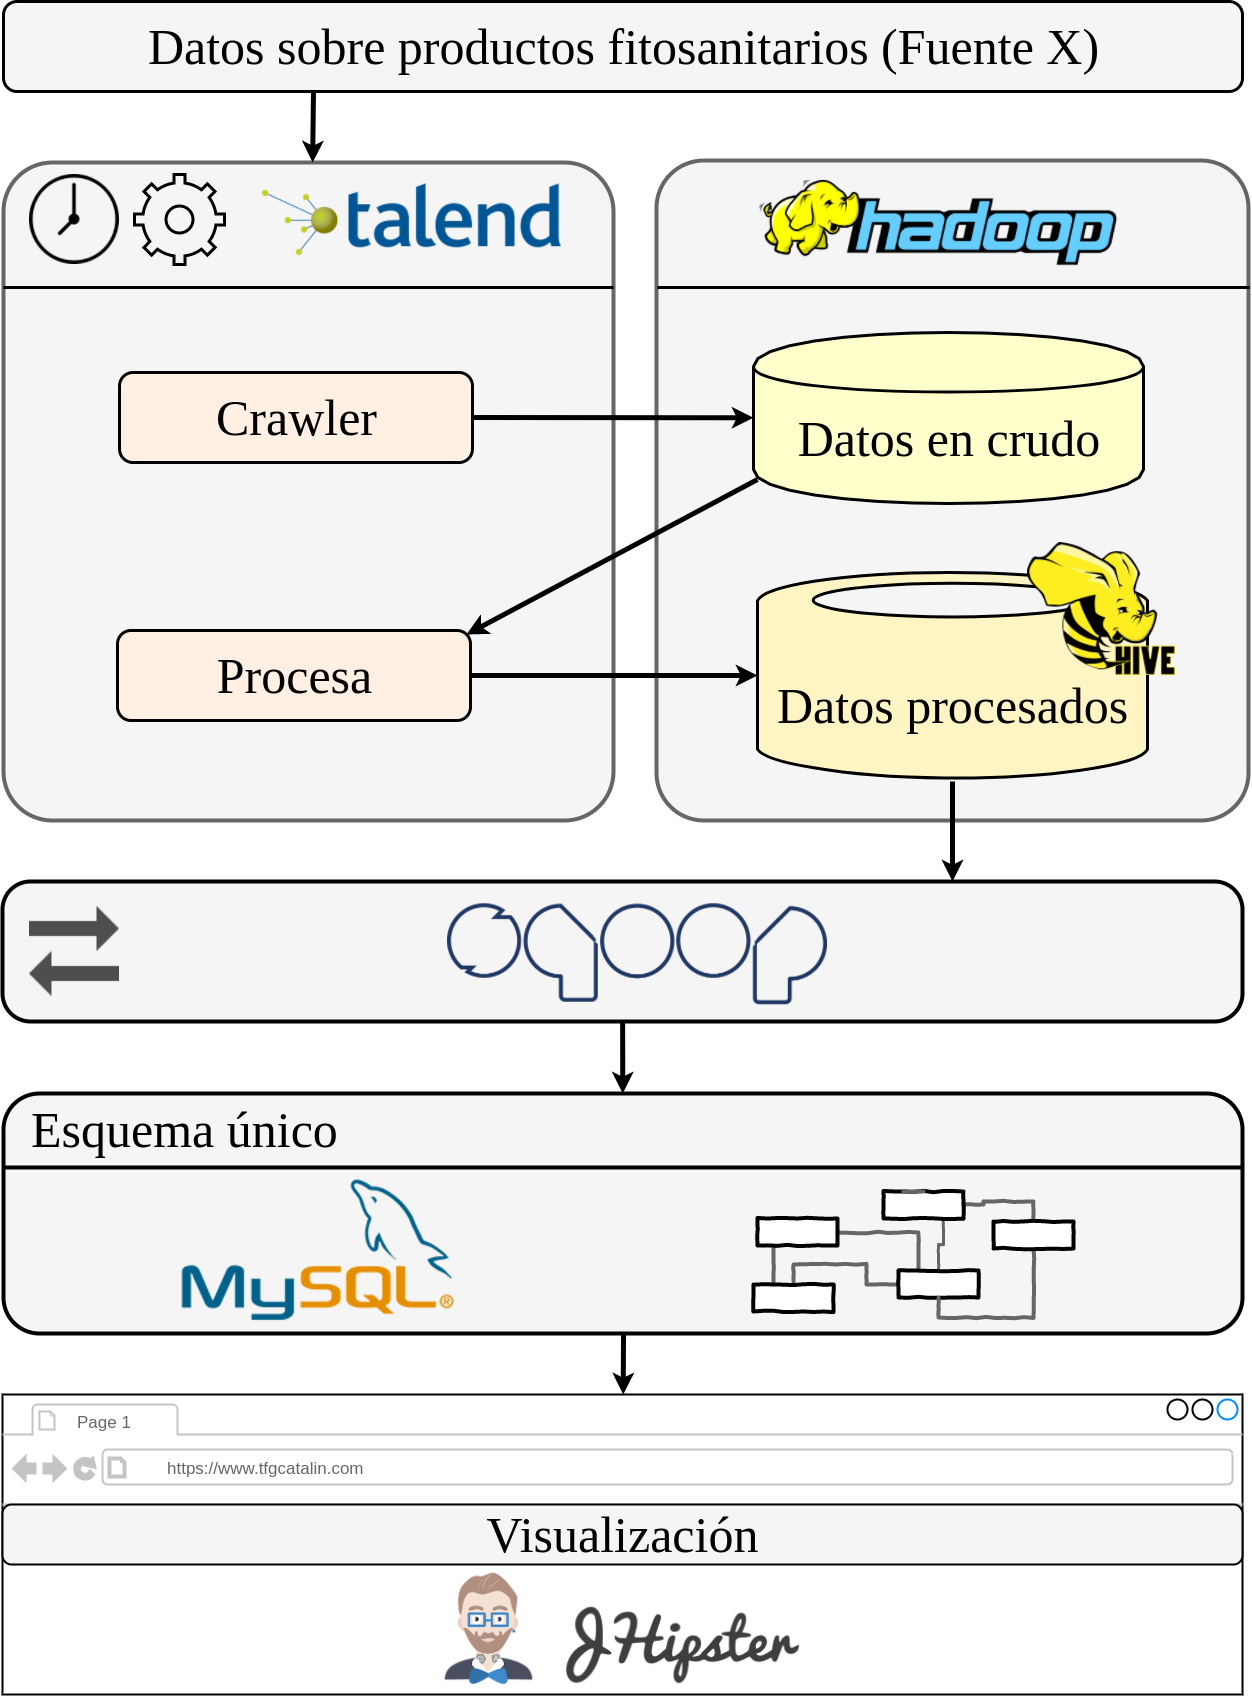
\includegraphics[width=1\textwidth,height=15cm,keepaspectratio]{Imagenes/disenyofinal}
    \caption{Diseño final de la solución - De los datos a su explotación}
    \label{fig:disenyofinal}
\end{figure}

\section{Arquitectura del sistema} \label{disenyo.arquitectura}
\par Este apartado tratará de dar una visión arquitectural del sistema, pasando por diferentes diagramas para representar el proyecto de manera gráfica y completa. Esta sección abarcará los siguientes diagramas: diagrama de despliegue, diagrama de componente y conector, diagrama de clases y paquetes, diagrama de secuencia y diagrama de datos. 

\subsection{Diagrama de despliegue.} \label{disenyo.arquitectura.despliegue}
\par Como se puede observar en la figura \ref{fig:despliegue}, el despliegue de la aplicación consta de un nodo principal, el Servidor. Este almacena tanto la aplicación de \textit{JHipster} como la base de datos \textit{MySQL} y \textit{Apache Sqoop}. La aplicación de \textit{JHipster}, al tratarse de una aplicación \textit{Spring} se representa como un artefacto dentro de un contenedor \textit{Spring}, el \textit{Spring Container}. Además, allí se define el módulo de \textit{schedulling} implementado por el alumno como un artefacto separado del de la aplicación, aunque a nivel práctico realmente su implementación está ubicada dentro del propio módulo de la aplicación. \textit{Apache Hadoop} aparece en el diagrama como una \textit{base de datos} aparte, por varias razones: en primer lugar, \textit{Apache Hadoop} se puede desplegar en un nodo separado del Servidor. En segundo lugar, se pueden crear varias instancias en diferentes nodos del mismo para conseguir almacenar una cantidad mayor de datos, y proporcionar la aplicación de un componente de almacenamiento escalable.
\begin{figure}[H]
    \centering
    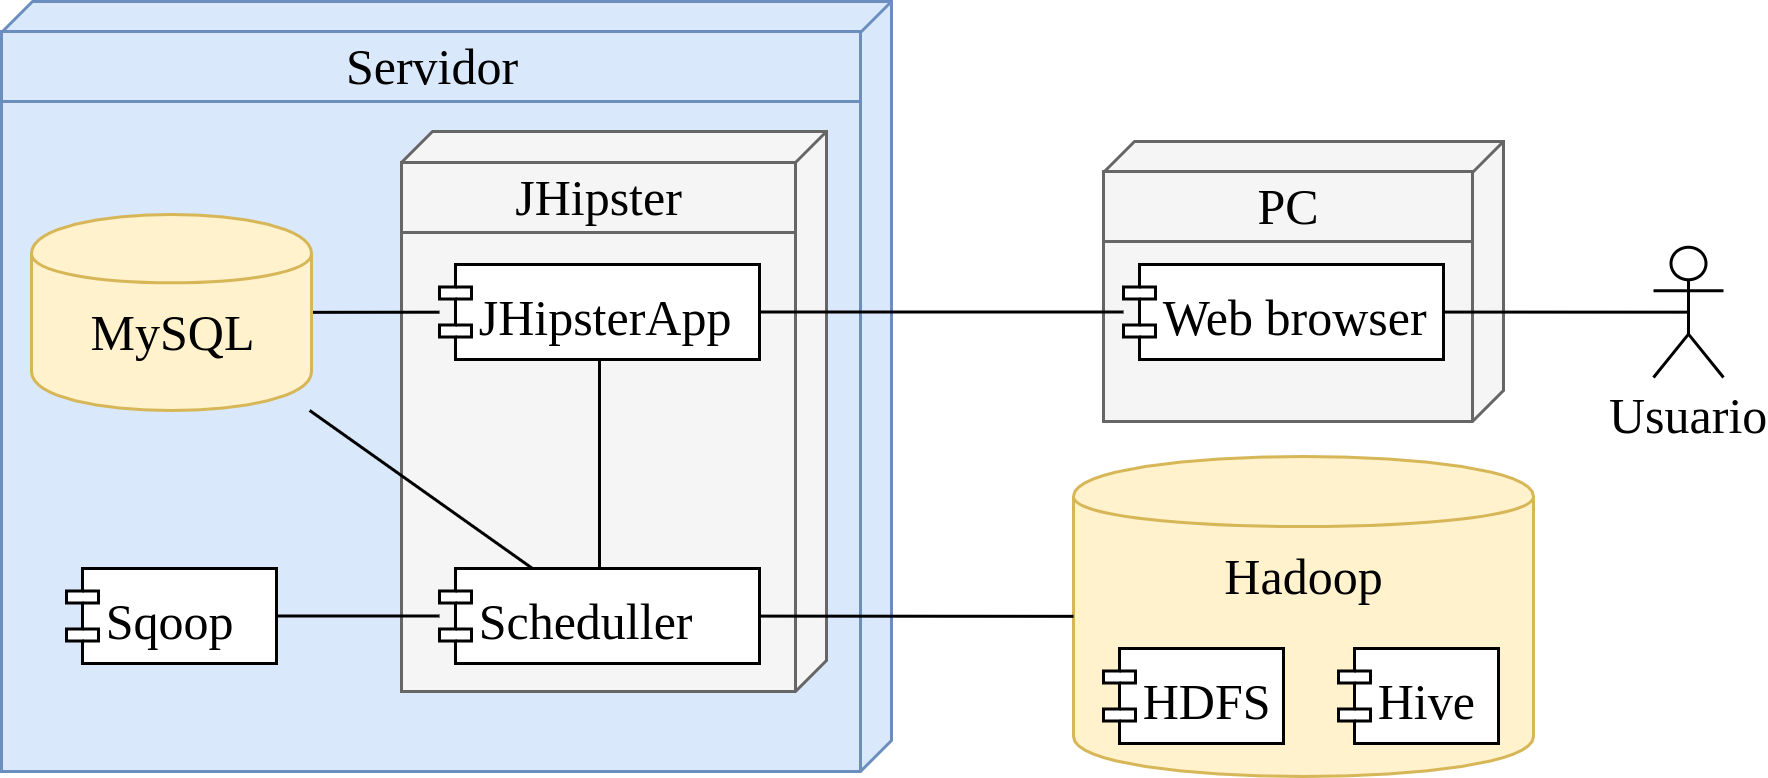
\includegraphics[width=1\textwidth,height=15cm,keepaspectratio]{Imagenes/despliegue}
    \caption{Diagrama de despliegue de la solución}
    \label{fig:despliegue}
\end{figure}

\subsection{Diagrama de componente y conector.} \label{disenyo.arquitectura.cyc}
\par El diagrama de la figura \ref{fig:cyc} muestra la visión arquitectural del sistema a nivel de componentes y conectores. En él se representan todos los elementos del sistema junto con las interfaces que ofrecen y utilizan cada uno de ellos. Se observan todas las conexiones que hay entre los distintos componentes y se puede interpretar como una expansión, o una visión de más bajo nivel del diagrama de despliegue. Se entiende el componente \textit{Talend} como los distintos procesos desarrollados con esta herramienta, más que una conexión con el propio programa ya que en ningún momento se requiere de \textit{Talend} más allá que para la construcción de dichos procesos. 

\begin{figure}[H]
    \centering
    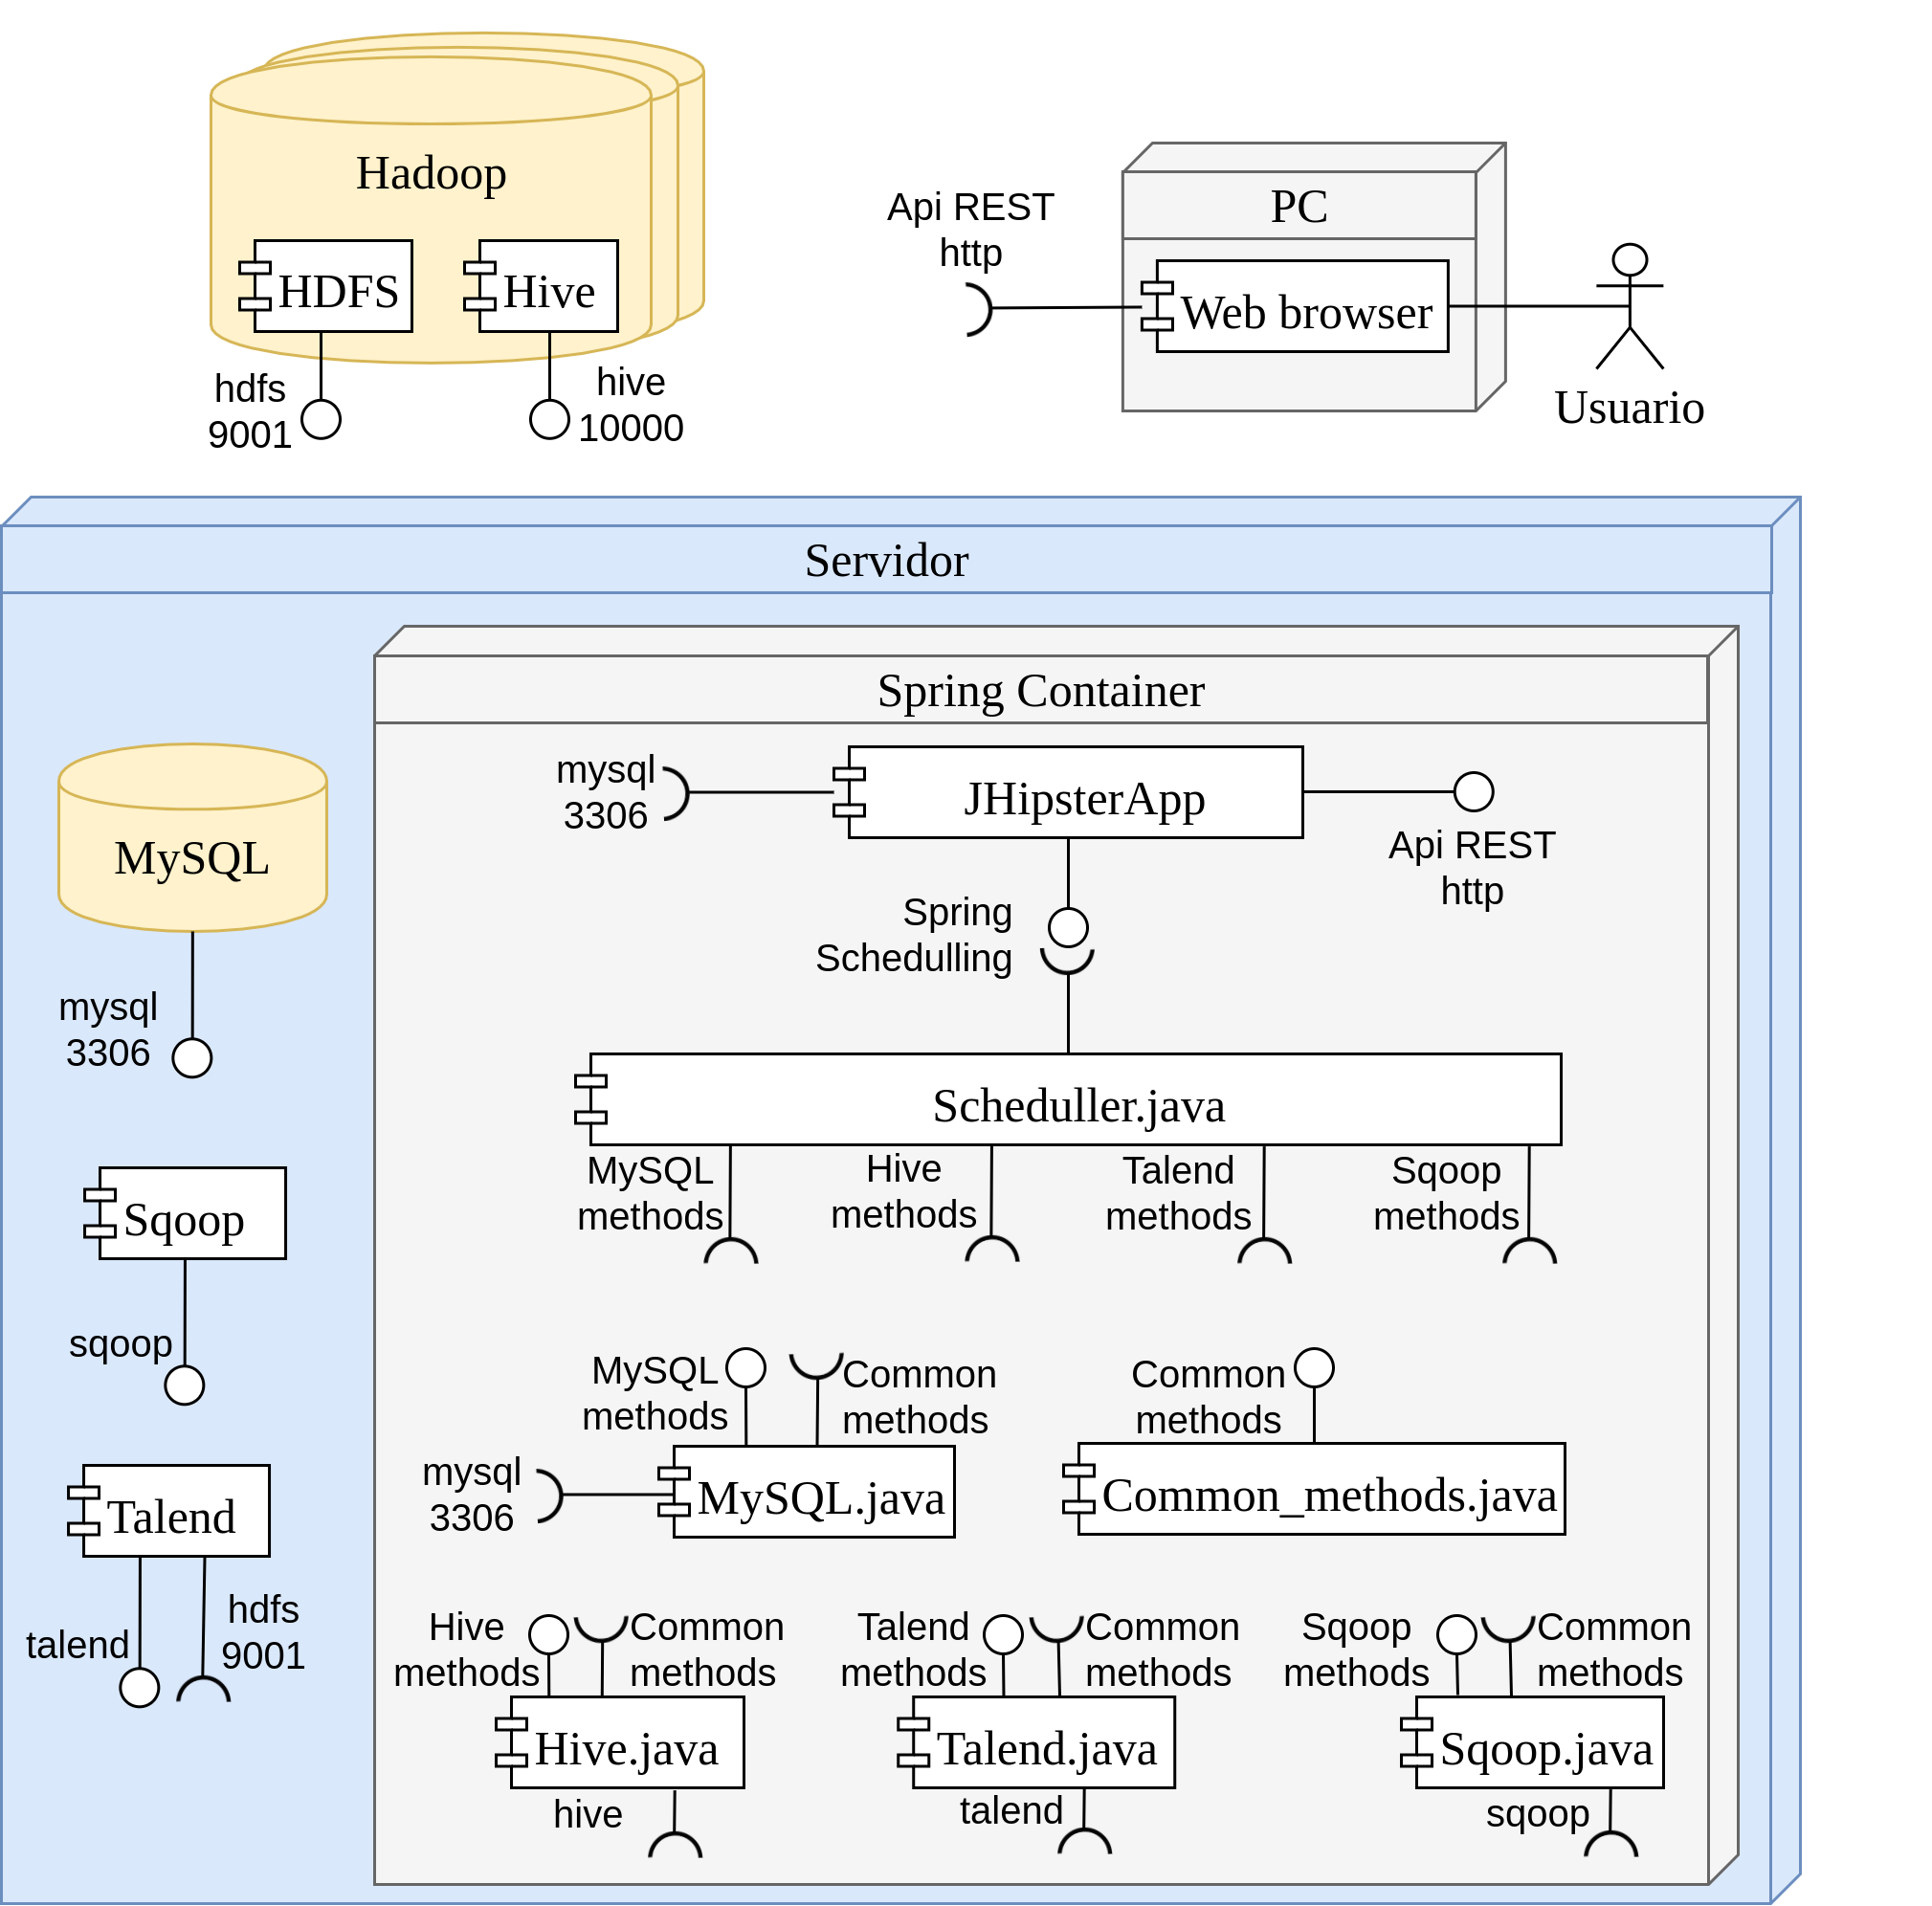
\includegraphics[width=\textwidth,height=\textheight,keepaspectratio]{Imagenes/cyc}
    \caption{Diagrama de componente y conector}
    \label{fig:cyc}
\end{figure}


\subsection{Diagrama de clases y paquetes.} \label{disenyo.arquitectura.clases}
 En el diagrama de clases presente en la figura \ref{fig:diag_clases} se adjunta el modelo de clases y paquetes correspondiente a la infraestructura que se construyó para soportar el comportamiento mencionado en la sección Implementación del prototipo real (Sección  \ref{implementacion.prototipo}). Dicho diagrama no incluye aquellas partes del código que se generan durante la instanciación de la aplicación con \textit{JHipster} sino únicamente las que el alumno ha desarrollado. 


\begin{figure}[H]
    \centering
    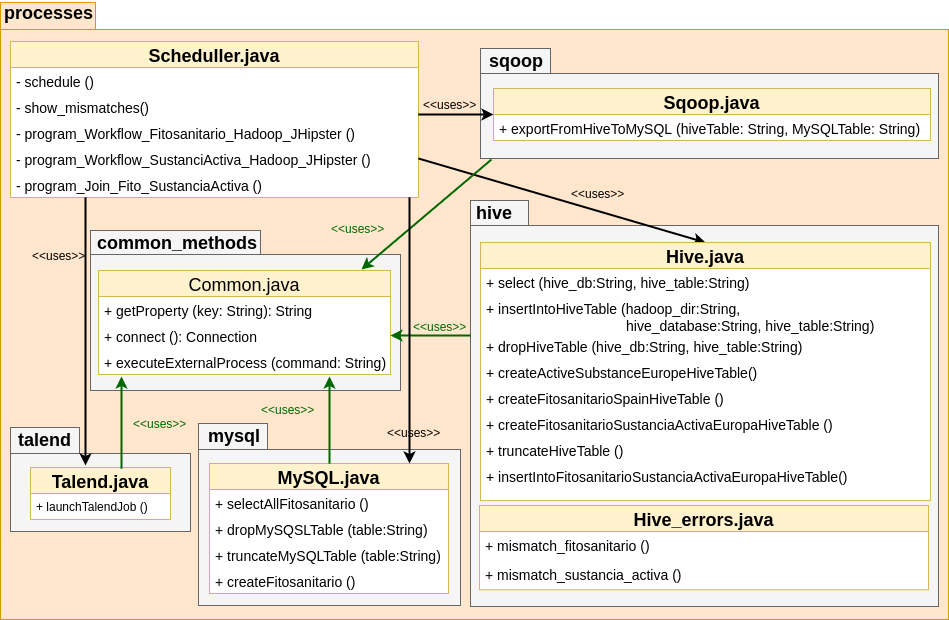
\includegraphics[width=\textwidth,height=\textheight,keepaspectratio]{Imagenes/clases}
    \caption{Diagrama de clases y paquetes para soportar la automatización del \textit{workflow}}
    \label{fig:diag_clases}
\end{figure}

\subsection{Diagrama de secuencia.} \label{disenyo.arquitectura.secuencia}
\par Una vez vista la estructura del diagrama anterior, a continuación se presenta un diagrama de secuencia de ejemplo para ilustrar la interacción de los diferentes componentes y el rol que juegan en el \textit{workflow} desde que los datos se descargan hasta que pasan a visualizarse mediante \textit{JHipster} Para ello se ha hecho uso de un ejemplo \textit{vertical} para los datos de los productos fitosanitarios autorizados de España. Periódicamente, los datos se descargan desde la web del \textit{MAPAMA} \cite{mapama}, son procesados y almacenados en \textit{Apache Hadoop}, se exponen en \textit{Apache Hive}, se transfieren con \textit{Apache Sqoop} a \textit{MySQL} y \textit{JHipster} es capaz de visualizarlos.

\begin{landscape}
\begin{figure}[p!]
    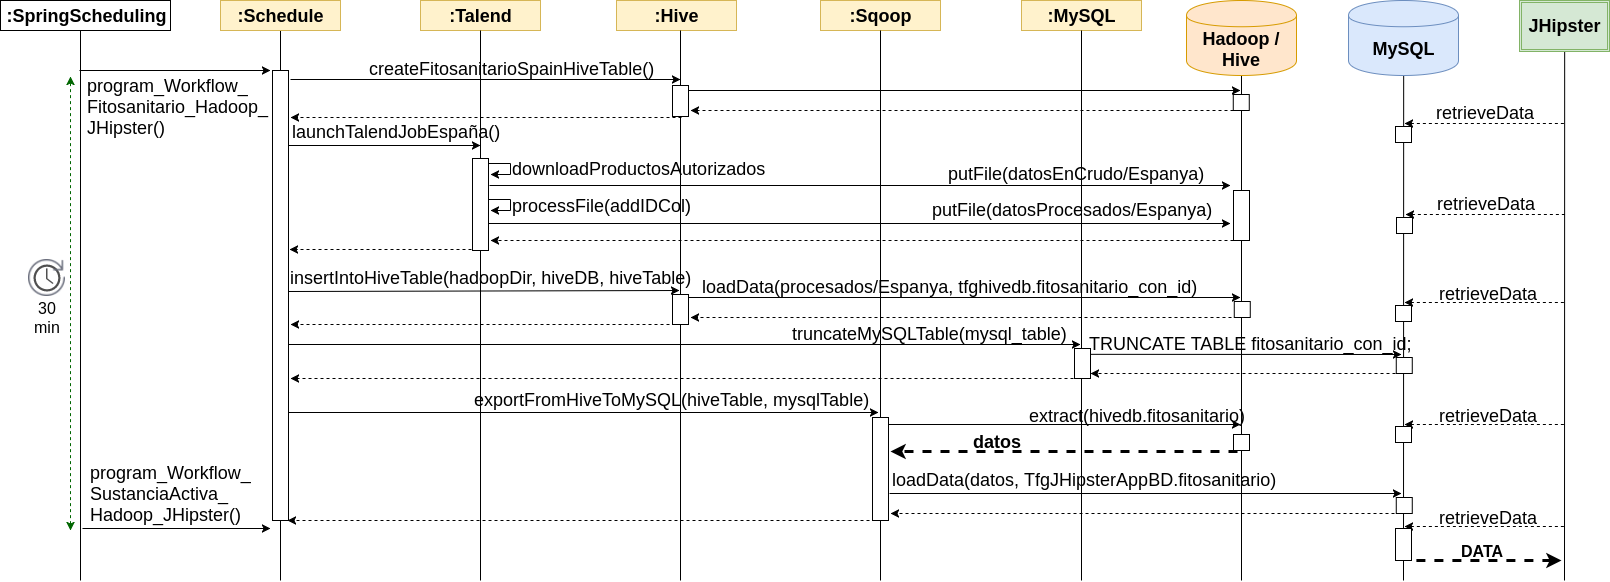
\includegraphics[width=\linewidth]{Imagenes/secuencia}
    \caption{Diagrama de secuencia del \textit{workflow} implementado}
    \label{fig:diag_secuencia_workflow}
\end{figure}
\end{landscape}
\bigskip


\subsection{Diagrama de datos.} \label{disenyo.arquitectura.datos}
\par A continuación se muestra el diagrama de datos tal como están almacenados en \textit{Apache Hive}. A pesar de que también se almacenan datos en la base de datos \textit{MySQL}, la estructura presente allí es relativamente sencilla en comparación con la de \textit{Apache Hive} y por lo tanto se ha decidido presentar en los anexos, en la sección \ref{a.datos.modelo}. 
\par 
Como se puede observar, en la figura \ref{fig:datosApache Hive} aparecen, mediante una estructura de diagrama entidad-relación las entidades que han sido creadas en \textit{Apache Hive}. Por una parte tenemos las entidades \textit{fitosanitario\_con\_id} y \textit{sustancia\_activa\_europa}, que son las entidades principales de la solución. La primera se crea a partir de los datos obtenidos de la primera fuente integrada en el proyecto, proveniente del listado de productos fitosanitarios autorizados en España disponibles en la página web del \textit{MAPAMA} \cite{mapama}. La segunda son los datos de las sustancias activas provenientes de la base de datos abierta sobre pesticidas a nivel europeo. El resto de entidades presentes en el modelo son el resultado de diferentes operaciones sobre estas dos tablas. A continuación se explica cómo se han conseguido dichas entidades y qué representan. 
\begin{enumerate}
\item En primer lugar, la relación marcada con un \textit{1} en el diagrama representa una cierta similitud en el campo \textit{formulado} de la primera tabla y el campo \textit{name} de segunda: El \textit{formulado} incluye el \textit{name} de la segunda tabla. No obstante, los datos no son perfectos: por una parte está el problema del idioma; muchos de los fitosanitarios aparecen en español mientras que las sustancias activas están en inglés, por lo que un mapeo directo no daría el 100\% de los \textit{matches}. Otro problema es el de los \textit{campos múltiples}, esto es, en la primera tabla, algunos registros del campo \textit{formulado} incluyen no solo uno, sino varios nombres de sustancias activas. Por lo tanto, haría falta una búsqueda para poder hacer el matching con todas las sustancias activas encontradas.
\item La relación marcada con un \textit{2} representa la tabla \textit{fito\_active\_substance}, que es el resultado de hacer un mapeo casi directo de la relación mencionada en el punto anterior: Primero, del campo \textit{formulado} nos quedamos únicamente con el nombre de la sustancia activa. Después se hace una operación de \textit{JOIN} para conseguir el \textit{real\_id} (id real de la sustancia activa) de la segunda tabla.
\item Las relaciones marcadas con un \textit{3} y un \textit{4} surgen de la necesidad de registrar los errores; las tablas \textit{mismatch\_fitosanitario\_fito\_sustancia} y \textit{mismatch\_sustancia\_fito\_sustancia} recogen aquellos fitosanitarios de la primera tabla que no aparecen en la tabla \textit{integrada} (\textit{fito\_active\_substance}) y aquellas sustancias activas de la segunda tabla que tampoco aparecen, respectívamente.
\end{enumerate}

\begin{landscape}
\begin{figure}[p!]
    \centering
    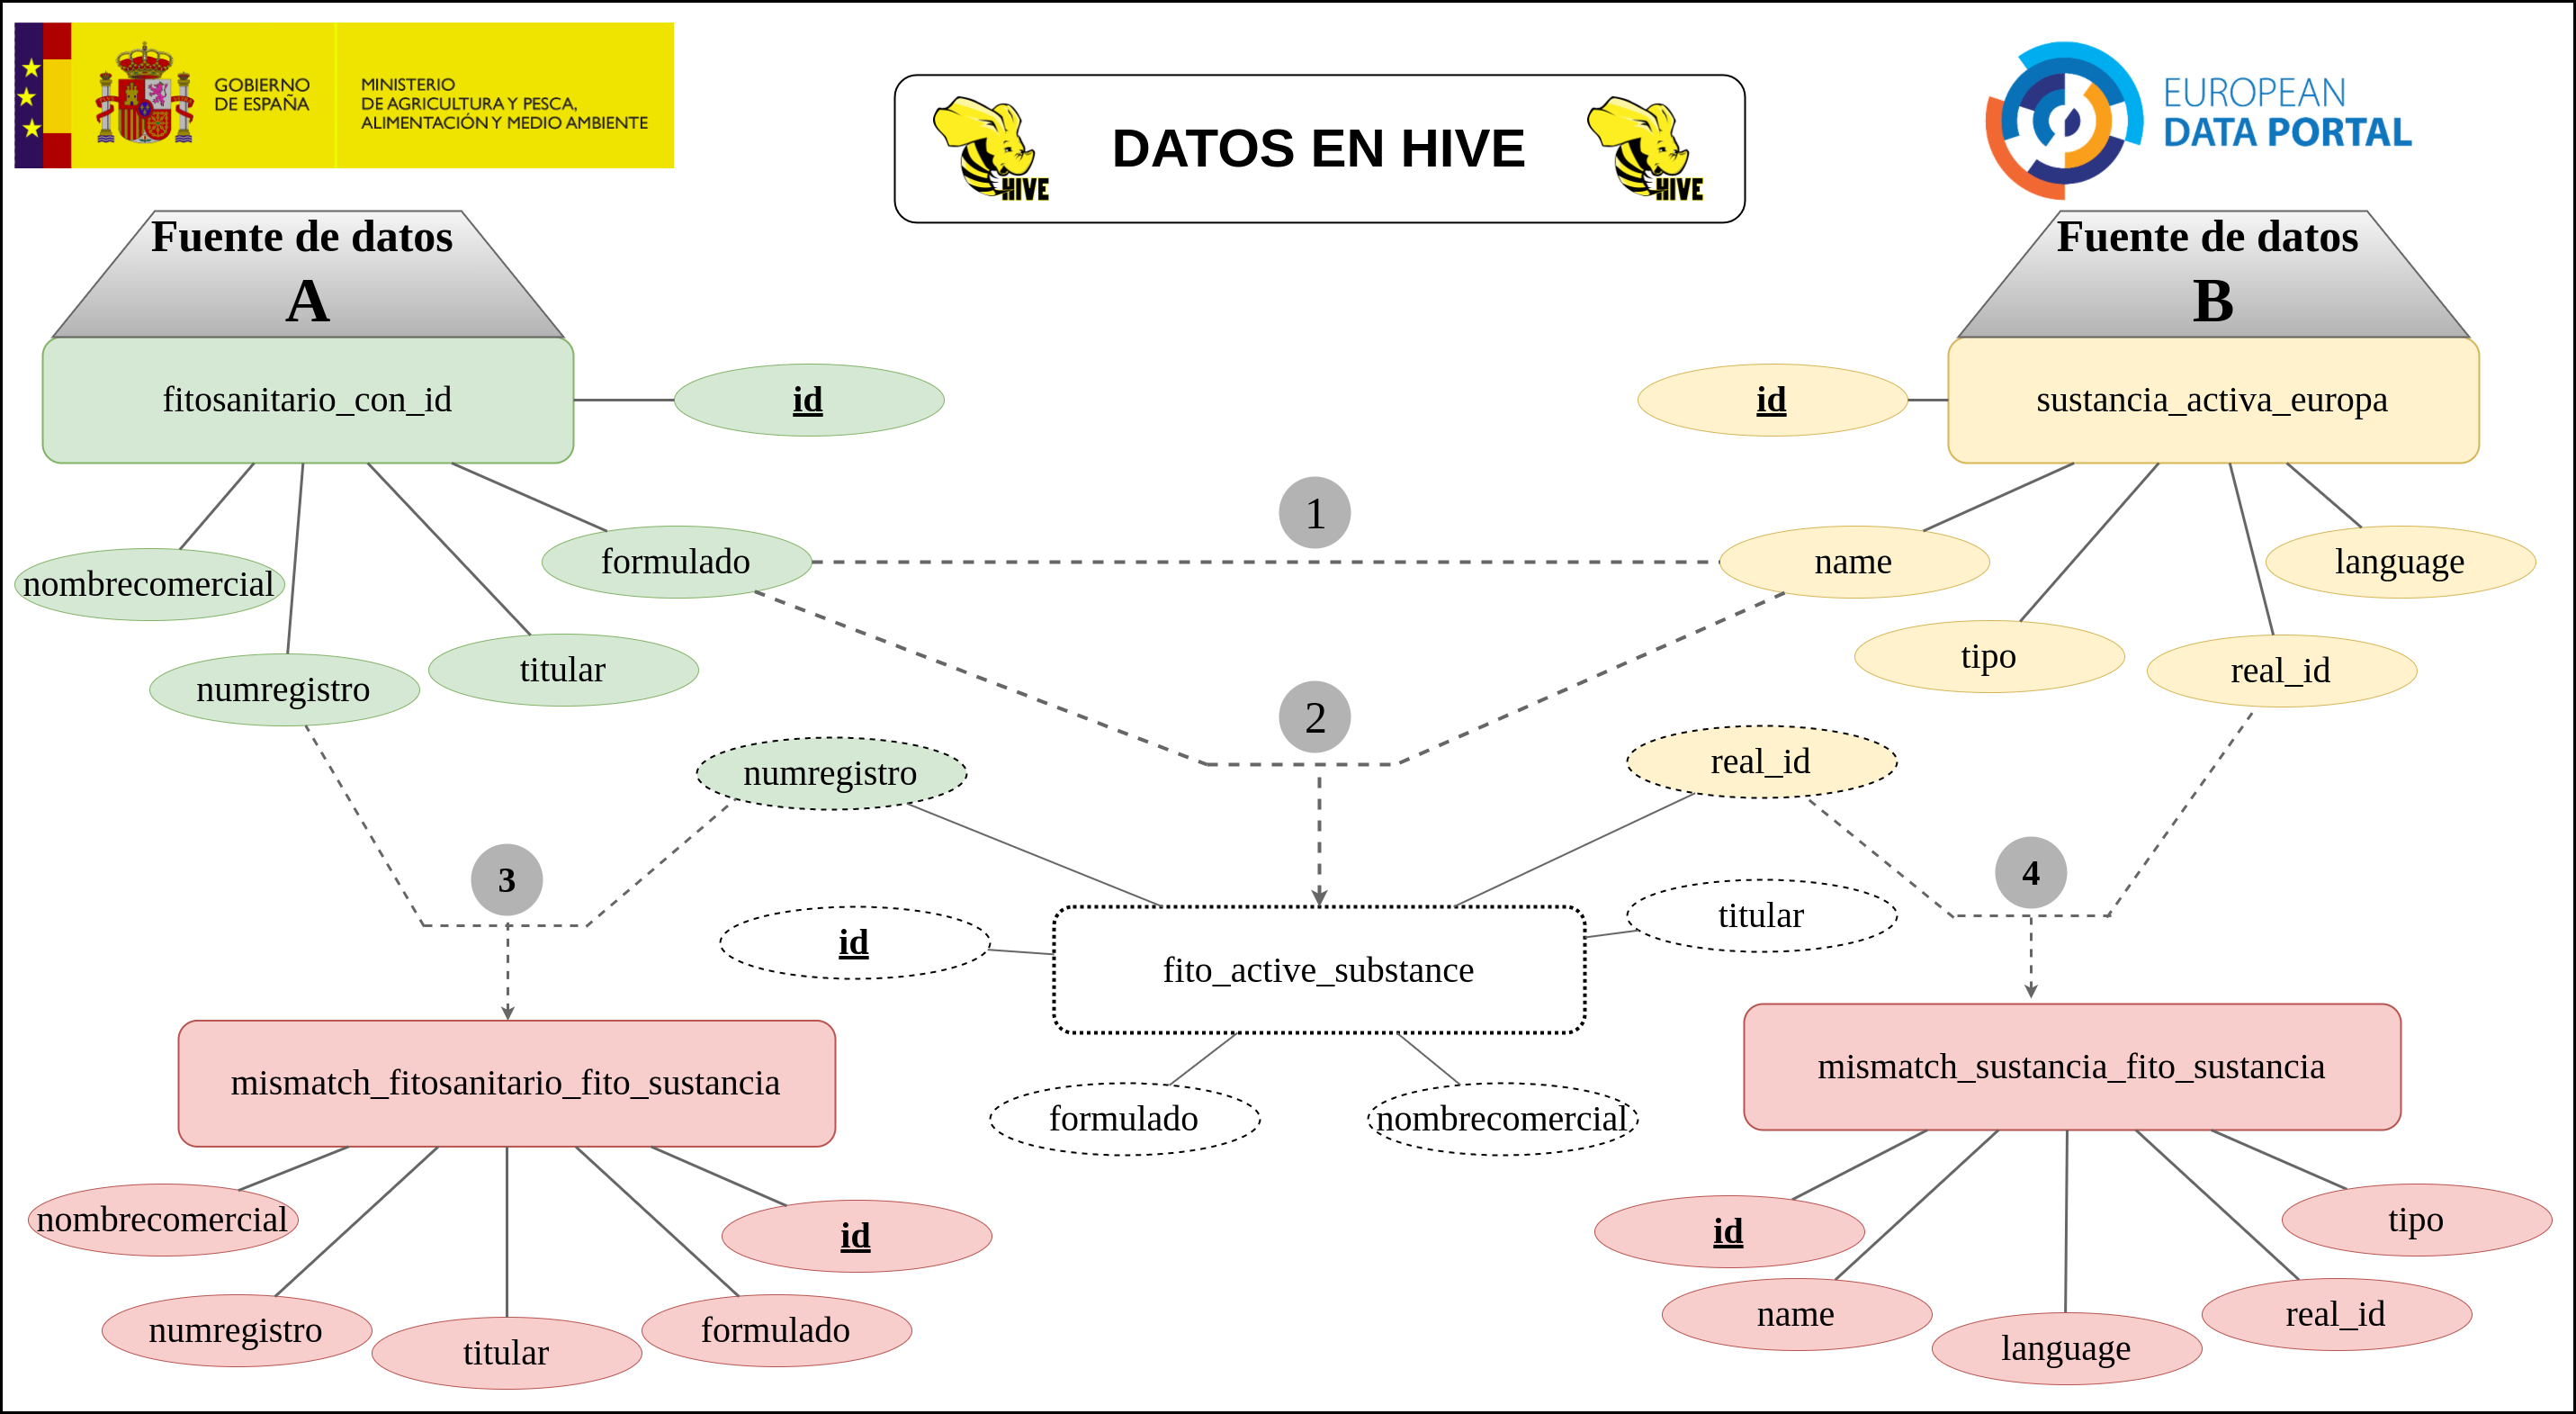
\includegraphics[width=\linewidth]{Imagenes/datoshive}
    \caption{Esquema de datos importados en \textit{Apache Hive}}
    \label{fig:datosApache Hive}
\end{figure}
\end{landscape}





\section{Estrategia de integración y expansión}
\label{disenyo.estrategia}

Una vez visto el diseño del sistema, en esta sección se hablará de la estrategia de integración y expansión que gobernará los futuros desarrollos a partir de la infraestructura montada en la realización de este proyecto. 

Como se observará en el desarrollo del prototipo real de la sección \ref{implementacion.prototipo}, realmente gracias a la infraestructura conseguida y a la arquitectura que se ha montado, realizar nuevas funcionalidades y expandir el proyecto no debería suponer un reto y debería ser bastante asequible. En este apartado caben destacar varias líneas posibles de expansión en el proyecto: 

\paragraph*{Aumento de la capacidad de almacenamiento.} Este apartado es bastante trivial, puesto que gracias a \textit{Apache Hadoop}, esto se puede conseguir fácilmente. Tal como se ha comentado, \textit{Apache Hadoop} tiene el potencial de crecimiento mediante nodos adicionales, desplegados en la misma o en diferentes máquinas, con capacidad de almacenamiento extra. Así pues, para que el sistema escalase en cuanto a capacidad de almacenamiento, lo único que se tendría que hacer es desplegar más nodos de \textit{Apache Hadoop} para tener la información repartida en más espacio de almacenamiento. 

\paragraph*{Integración de datos nuevos.} Para integrar nuevos datos en el sistema de nuevas fuentes, la estrategia a seguir debería ser la que se observa en el diagrama de la figura \ref{fig:expansion}.

\begin{figure}[!h]
    \centering
    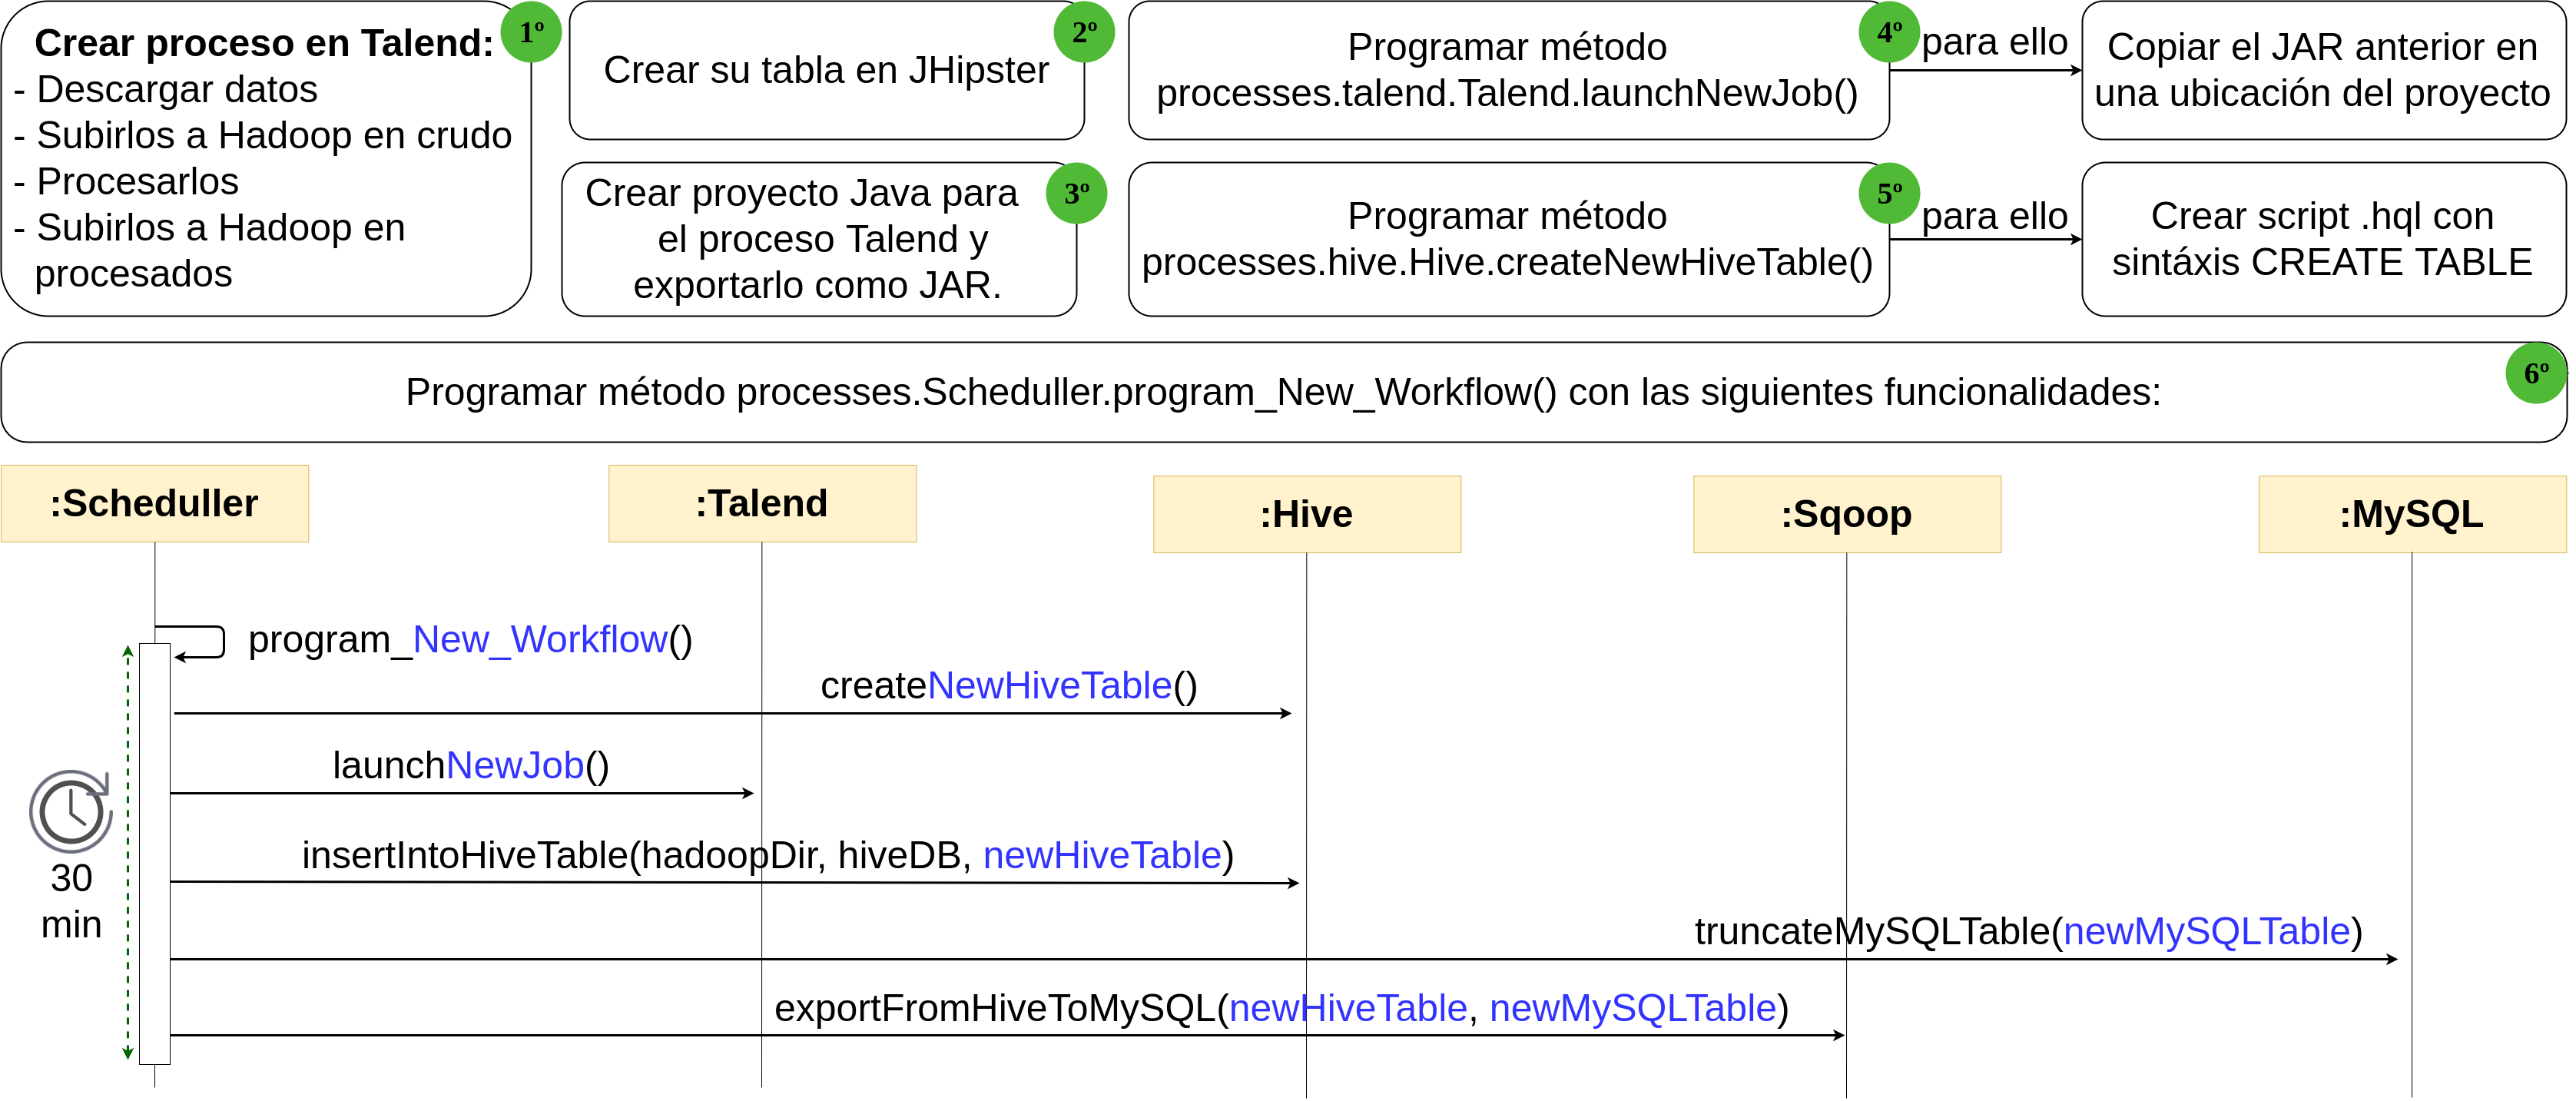
\includegraphics[width=\textwidth,height=\textheight,keepaspectratio]{Imagenes/expansion}
    \caption{Estrategia recomendada para la integración de datos nuevos}
    \label{fig:expansion}
\end{figure}
\textbf{Funcionalidades extra.} Aunque realmente este proyecto se ha desarrollado pensando en una expansión futura únicamente en cuanto a la integración de nuevos datos y la escalabilidad de almacenamiento, gracias a la estructura de la aplicación de \textit{JHipster} es posible dotar al sistema de tantas funcionalidades extra como se desee. 

\section{Restricciones al diseño} \label{disenyo.restricciones}
La gestión y desarrollo del proyecto, en todas sus fases se ha visto restringida por diferentes pautas y recomendaciones provenientes de terceras partes. Este apartado pretende aclarar algunas de estas cuestiones para reflejar aquellas decisiones que han condicionado, para bien o para mal, el desenvolvimiento del alumno. 
\par Desde el inicio del proyecto el director impuso algunas de las herramientas a utilizar, así como el diseño a priori de la solución. \textit{Apache Hadoop}, \textit{Apache Hive} y \textit{JHipster} fueron el \textit{core} tecnológico que el director estableció para la realización del proyecto. Como primer diseño, además, el director expuso un modelo en el que los datos tanto procesados como sin procesar serían almacenados en \textit{Apache Hadoop}, consumidos desde \textit{Apache Hive} e importados directamente a \textit{JHipster}, sustituyendo la base de datos de \textit{JHipster} por \textit{Apache Hive}. Tras observar que este modelo no cumplía con los requisitos del proyecto, se optó por la otra variante, mediante \textit{Apache Sqoop}, tal como se ha mencionado anteriormente. 
\par Otra de las herramientas recomendadas por el director del proyecto fue \textit{Pentaho Kettle} y, como se puede observar en la sección \ref{implementacion.problemas}, fue una de las piezas que más problemas acabó dando. Ante esta situación, el director recomendó \textit{Talend}, que resultó ser un mejor componente y que satisfacía con los requisitos de la fase de análisis.
\par Otro aspecto que se debe tener en cuenta es que el proyecto se trata de un \textit{TFG} y no de una solución comercial. Por ello, hay unas normas o pautas  establecidas que delimitan y guían en el desarrollo del mismo: la limitación de las horas de dedicación recomendadas, que se corresponden a los 12 créditos ECTS, la inclusión de una memoria suficientemente extensa para recopilar todos los aspectos del desarrollo del proyecto e incluso la limitación económica implícita, esto es, no existe una remuneración monetaria para el alumno tras el desarrollo del proyecto. 






\chapter{Implementación} \label{implementacion}
\section{Prueba de concepto} \label{implementacion.prueba}

La primera fase de desarrollo de la solución fue la prueba de concepto; su objetivo fue encontrar las herramientas adecuadas para el \textit{Stack Tecnológico} y demostrar que las elegidas son viables y que funcionan en conjunto. Además, se estudiaron y valoraron los problemas que puedan presentar y los retos que podrían suponer desde una aproximación tecnológica. Conceptualmente, este apartado podría verse englobado dentro de la sección de Análisis (Capítulo \ref{analisis}) ya que, como se ha mencionado, la prueba de concepto fue la que determinó el \textit{Stack Tecnológico} y, por ende, incluyó una correspondiente parte de análisis, esto es, búsqueda, investigación, test de viabilidad, etc. No obstante, dado que realmente formó parte del desarrollo de la solución se ha decidido redactarlo como una primera parte del apartado de Implementación de la solución. Así pues, esta sección presentará tanto el \textit{Stack Tecnológico} utilizado, los problemas encontrados en esta fase y las diferentes alternativas que se han probado junto con los motivos por los que se han desechado de la decisión final. En el diagrama de la figura \ref{fig:pruebaconceptoglobal} se puede observar el panorama global de los pasos que se han dado y las herramientas que se han utilizado para montar toda la infraestructura necesaria para una versión final de la prueba de concepto dentro de la primera fase del desarrollo del proyecto. 
\par Después se hará un breve resúmen de las pruebas que se han realizado con las diferentes herramientas consideradas como partes potenciales del \textit{Stack Tecnológico}, que será ampliado en la sección \ref{e.disenyo.pruebaconcepto} de los anexos.
\begin{landscape}

\begin{figure}[p!]
    
    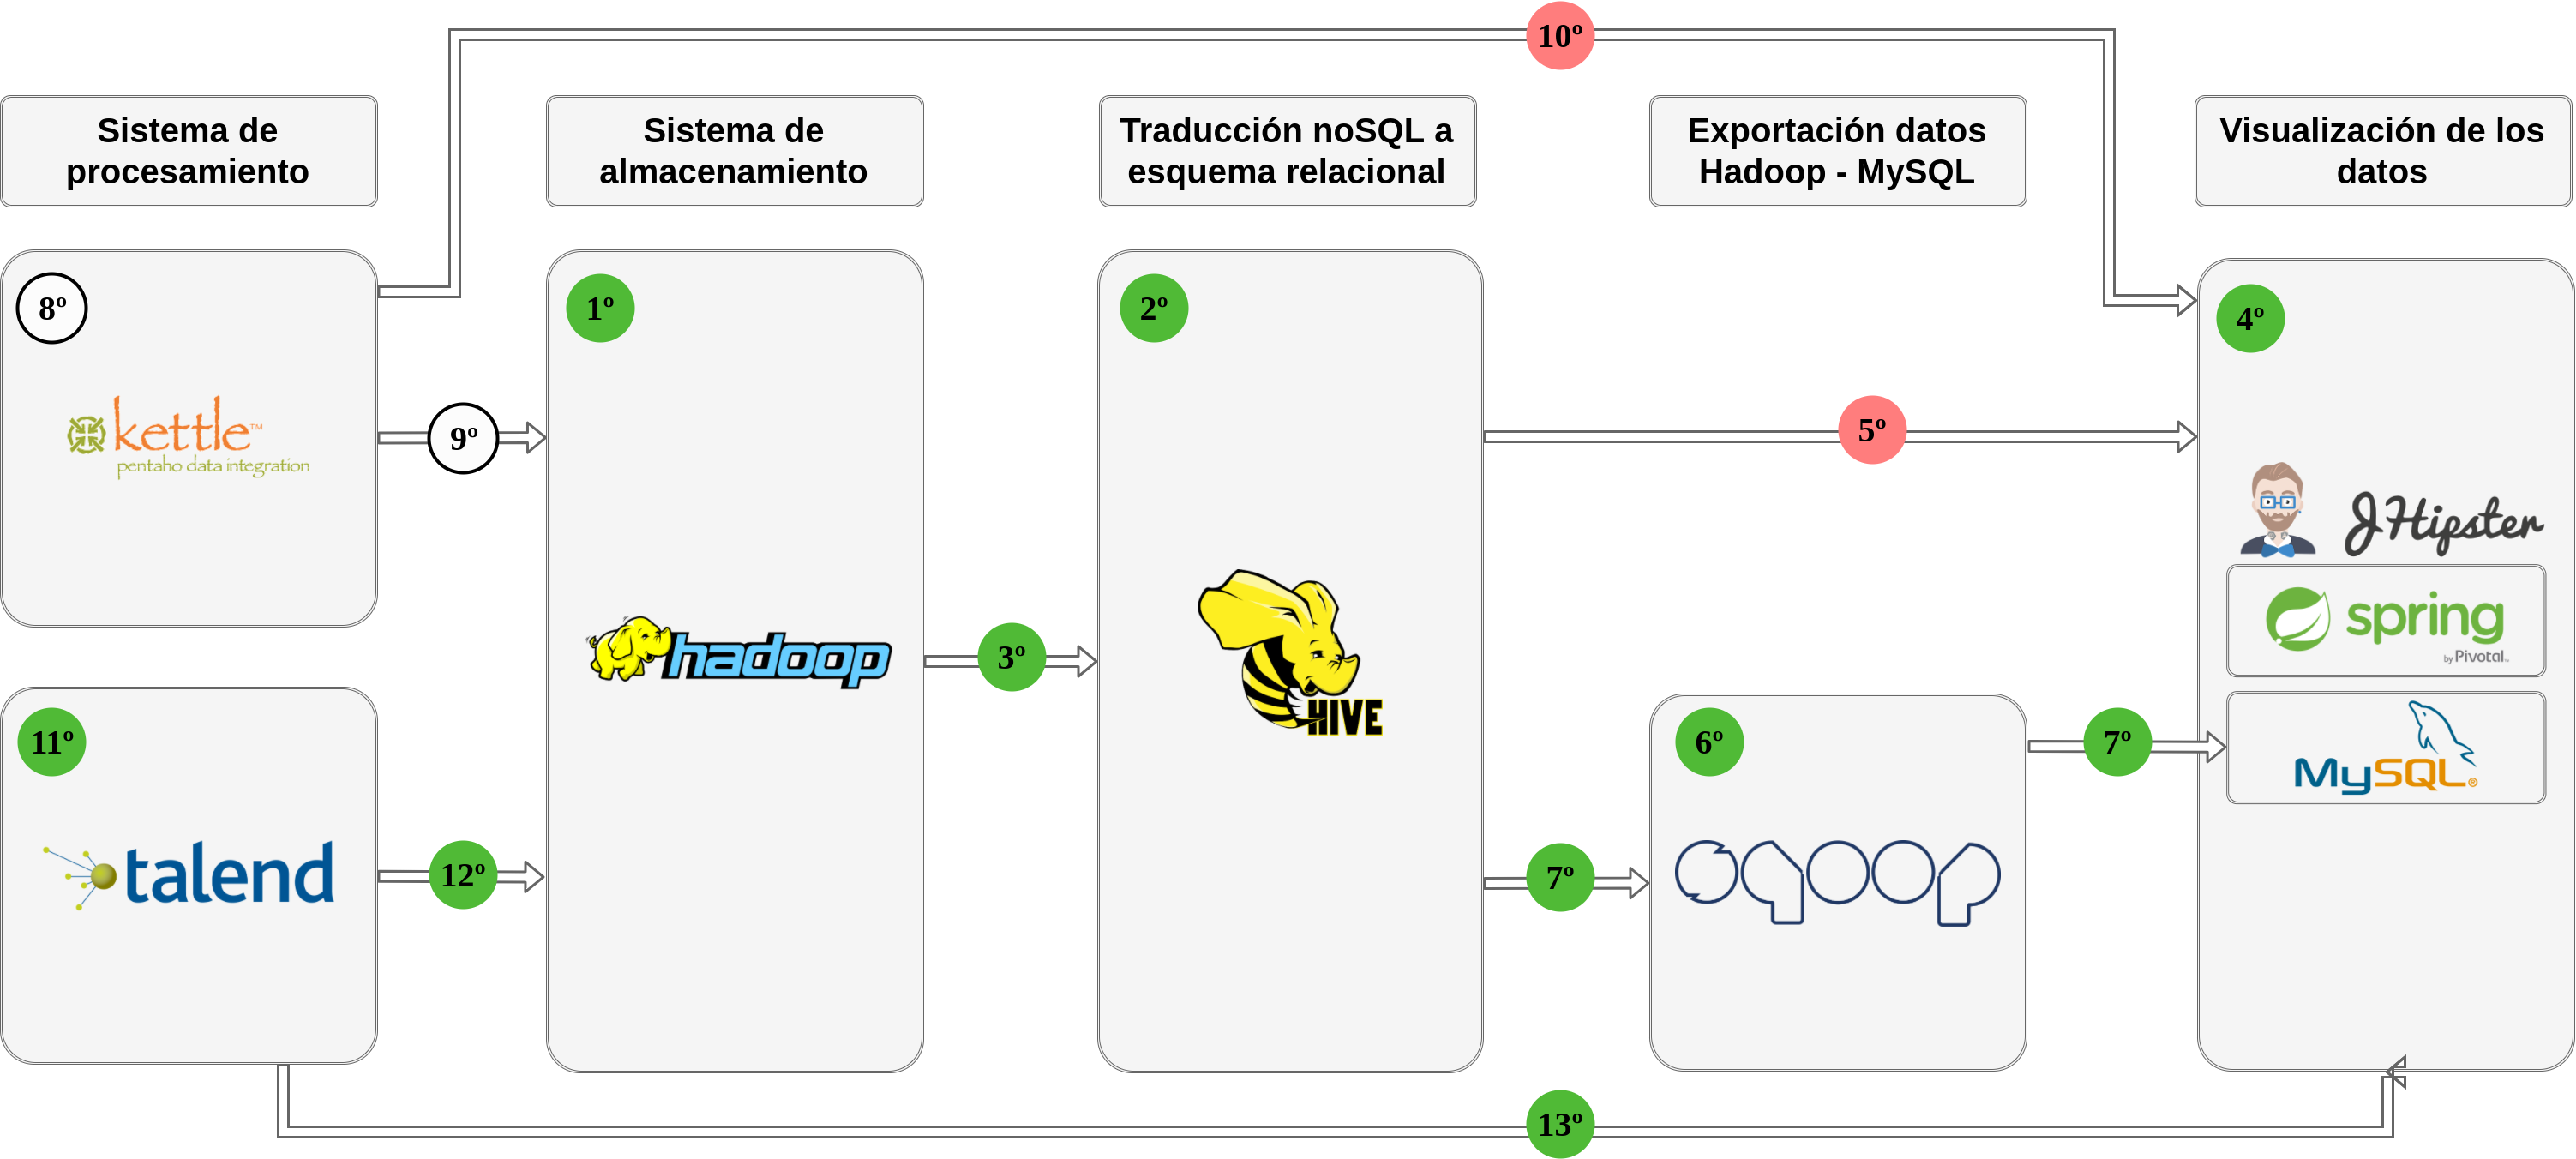
\includegraphics[width=\linewidth]{Imagenes/pruebadeconceptoglobal}
    \caption{Diagrama de las etapas de la prueba de concepto.}
    \label{fig:pruebaconceptoglobal}
\end{figure}

\end{landscape}


\par

\textbf{Pasos reflejados en el diagrama de la figura \ref{fig:pruebaconceptoglobal}:}


\begin{table}[H]
\centering
\bgroup
\def\arraystretch{1.3}
\begin{tabular}{c p{280pt} c}
\toprule
\textbf{Paso} & \textbf{Descripción} & \textbf{Resultado} \\
 \midrule
 1º
& 
Instalación y configuración de \textit{Apache Hadoop}
& 
Éxito
 \\
 2º
& 
Instalación y configuración de \textit{Apache Hive}
& 
Éxito
 \\
 3º
& 
Configuración de la conexión de \textit{Apache Hadoop} con \textit{Apache Hive}
& 
Éxito
 \\
 4º
& 
Instalación y configuración de \textit{JHipster}
& 
Éxito
 \\
 5º
& 
Intento de conexión directa entre \textit{JHipster} y \textit{Apache Hive}
& 
Resultado fallido.
 \\
 6º
& 
Instalación y configuración de \textit{Apache Sqoop}
& 
Éxito
 \\
 7º
& 
Exportación de datos desde \textit{Apache Hive} a \textit{MySQL} con \textit{Apache Sqoop}
& 
Éxito
 \\
 8º
& 
Instalación y configuración de \textit{Kettle Pentaho}
& 
Éxito
 \\
 9º
& 
Desarrollo de procesos \textit{ETL} para \textit{Apache Hadoop} mediante \textit{Kettle Pentaho}
& 
Éxito
 \\
 10º
& 
Intento de importación de procesos de \textit{Kettle Pentaho} en \textit{JHipster}
& 
Resultado fallido
 \\
 11º
& 
Instalación y configuración de\textit{ Talend Big Data}
& 
Res
 \\
 12º
& 
Desarrollo de procesos \textit{ETL} para \textit{Apache Hadoop }mediante \textit{Talend Big Data}
& 
Éxito
 \\
 13º
& 
Importación de procesos de \textit{Talend Big Data} en \textit{JHipster}
& 
Éxito
 \\
\bottomrule
\end{tabular}
\egroup
\caption{Pasos realizados durante la prueba de concepto}
\label{tab:pasos_prueba_de_concepto}
\end{table}


\par
\paragraph*{Desarrollo de la prueba de concepto.}
Tal como se observa tanto en el diagrama como en los pasos anteriores, la prueba de concepto se llevó a cabo de una manera secuencial, validándo primero las tecnologías y herramientas individuales y posteriormente intentando integrárlas. En primer lugar \textit{(pasos 1 y 2)} se instalaron y configuraron los componentes principales del proyecto: \textit{Apache Hadoop} y \textit{Apache Hive} y después se llevó a cabo su interconexión guiada por pruebas de traspaso de datos de \textit{Hadoop} a \textit{Hive} \textit{(paso 3)}. A continuación se instaló \textit{JHipster} \textit{(paso 4)} y en una primera aproximación al problema se intentó conectar diréctamente \textit{JHipster} con la base de datos \textit{Hive} \textit{(paso 5)}. Tras descubrir que este método no era adecuado pues \textit{JHipster} no ofrece ningún tipo de soporte \textit{ad hoc}, se optó por un cambio de estrategia; enlazar el flujo de datos entre \textit{Hive} y \textit{JHipster} mediante \textit{Sqoop}. Para ello se instaló, configuró y probó \textit{Sqoop} \textit{(pasos 6 y 7)} con resultados satisfactorios. Tras observar que el uso exclusivo de estas herramientas eran incompletas para el desarrollo del proyecto (puesto que se determinó necesario un programa de procesado, transformación y carga de ficheros), la opción más prometedora fue \textit{Kettle Pentaho} \textit{(paso 8)}. Si bien la construcción de los procesos mediante esta herramienta resultó una tarea no demasiado tediosa \textit{(paso 9)}, su traspaso a un programa \textit{Java} integrable dentro del proyecto de \textit{JHipster} resultó reiterádamente fallido \textit{(paso 10)}. Se decidió recurrir a otra prometedora herramienta, \textit{Talend Big Data} como sustitutiva de \textit{Kettle Pentaho}, lo que resultó en una gestión acertada \textit{(paso 11)}. 
Con \textit{Talend} se pudieron construir los procesos necesarios para transformar y transportar los datos desde/hacia \textit{Hadoop} \textit{(paso 12)} y se logró realizar el traspaso de dichos procesos a un programa \textit{Java} e integrarlo en \textit{JHipster} \textit{(paso 13)}.

\par
\paragraph*{Conclusiones.}

\par
Una vez conseguidos los pilares fundamentales de la integración dentro del proyecto (\textit{Hadoop}, \textit{Hive}, \textit{JHipster}, \textit{Sqoop}, \textit{Talend}) realmente las únicas preocupaciones que quedaban eran la automatización íntegra del proceso y la ejecución periódica del mismo para disponer de los datos en su versión actualizada. No obstante, para estas tareas no fue necesaria una prueba de concepto puesto que todo esto se podía conseguir desde el propio proyecto de \textit{JHipster}, mediante \textit{Spring} y código \textit{Java}, cosas con las que el alumno ya estaba familiarizado. Dándo por finalizada la prueba de concepto, se empezó a diseñar y construir el prototipo real que quedaría como solución real del proyecto.


\section{Prototipo} \label{implementacion.prototipo}
\par 
\textbf{Primera iteración para conseguir una integración y automatización completa - Productos fitosanitarios autorizados de España}
\bigskip
\par Lo primero que se hizo entrando en el desarrollo del prototipo real fue implementar un simple proceso mediante la interfaz gráfica de \textit{Talend}. Este proceso realiza las siguientes operaciones: 
\begin{enumerate}
\item Descarga desde la web del \textit{Mapama} el fichero \textit{Excell} de los productos fitosanitarios autorizados.
\item Convierte dicho \textit{Excell} a un formato \textit{OpenOffice} para poder ser procesado desde \textit{Talend} con los componentes excel correspondientes. 
\item Sube a Hadoop una versión sin procesar del fichero
\item Procesa el fichero añadiendole una columna llamada \textit{ID} al principio y lo sube como versión procesada a \textit{Hadoop}. 
\end{enumerate} 

A continuación se exportó el proceso desde Talend: 
\textit{Archivo $\rightarrow$ Export $\rightarrow$ Java $\rightarrow$ archivo JAR file}. Esto exporta las clases y librerias que \textit{Talend} necesita para lanzar el job en un archivo comprimido llamado \textit{nombre\_job.jar}
El siguiente paso fue descomprimir el \textit{archivo JAR} en cuestión, analizar su contenido y ver cómo se podría importar en un proyecto Java. El \textit{archivo JAR} contenía varias carpetas y ficheros pero lo que interesa es lo siguiente:
\bigskip
\par 
\dirtree{%
.1 Nombre\_del\_JAR.
.2 lib.
.3 \textit{librerias JAR}.
.2 Nombre\_del\_proyecto.
.3 Nombre\_del\_job.
.4 \textit{clase java principal del job}.
.2 routines.
.3 system.
.4 api.
.5 \textit{clases java}.
.4 xml.
.5 sax.
.6 \textit{clases java}.
.4 \textit{clases java}.
.3 \textit{clases java}.
}
\bigskip
\par
Así pues, a continuación se creó un nuevo proyecto \textit{Java} con \textit{IntelliJ} y \textit{Maven} (\textit{TalendCrawler}) y se copiaron todas las clases Java con su correspondiente estructura de carpetas. Dentro del fichero pom.xml del proyecto \textit{TalendCrawler} donde se importaron todas las dependencias de Talend que figuraban como librerías locales en la carpeta \textit{lib}. Para ello se tuvo que definir el \textit{repositorio de paquetes de Cloudera} \cite{cloudera}, que es desde donde Maven buscaría la mayoría de librerías. Tras comprobar que la aplicación arrancaba y se comportaba correctamente, el próximo paso fue encapsular y exportar la aplicación como un \textit{archivo JAR}, en conjunto con sus librerías. Para ello se hizo uso del plugin \textit{one-jar} de \textit{Maven} que recoge las dependencias del proyecto y las empaqueta junto a las otras clases en un único \textit{archivo JAR}.\par 

En el proyecto de \textit{JHipster} lo que se hizo fue crear una clase llamada Talend, desde la que periódicamente (mediante la anotación \textit{Scheduled}) se ejecutaba el \textit{archivo JAR} anterior a través del comando \textit{Runnable}. 

\begin{figure}[!h]
    \centering
    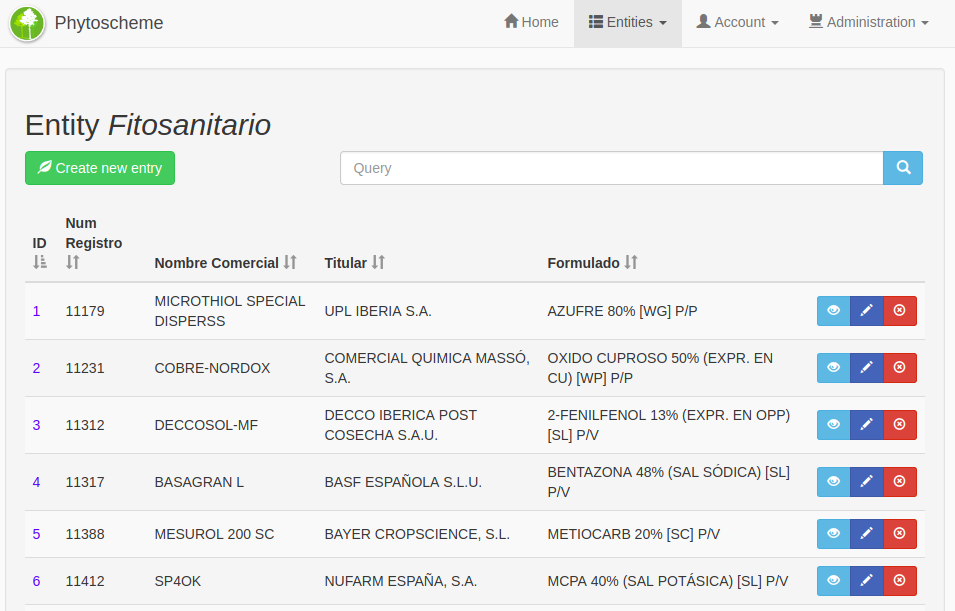
\includegraphics[width=\textwidth,height=\textheight,keepaspectratio]{Imagenes/capturaFitosanitarios}
    \caption{Captura de pantalla de la integración de los productos fitosanitarios.}
    \label{fig:capturaFitosanitarios}
\end{figure}

\par
Teniendo ya el proceso de \textit{Talend} integrado en la aplicación de \textit{JHipster}, el siguiente problema a abordar fue el de la automatización de su ejecución. Se sabe que los productos fitosanitarios autorizados son actualizados periódicamente en la web de \textit{MAPAMA}. Por eso mismo, nuestra aplicación requería también de una descarga periódica de dichos datos, para asegurarse de que en todo momento el programa tiene la versión actualizada de los fitosanitarios autorizados de España. Esto se consiguió gracias al \textit{módulo de scheduling}\cite{spring_scheduling} de \textit{Spring} que permite programar la ejecución de un método de manera periódica. Como decisión estratégica se propuso lanzar el proceso de \textit{Talend} cada media hora. Resuelto este problema también, el siguiente objetivo fue automatizar toda la ejecución del proceso, desde la descarga del fichero de los productos autorizados hasta la visualización de los datos mediante \textit{JHipster}. Aprovechandose del mismo módulo anterior de \textit{scheduling}, el desarrollo tendría que seguir el siguiente esquema: 
\begin{itemize}
\item Primero, los datos deberían descargarse y procesarse y almacenarse en \textit{Hadoop} mediante el módulo de \textit{Talend}.
\item A continuación, se debería implementar otro módulo encargado de la carga de dichos datos procesados a una tabla de \textit{Hive}.
\item Después de eso, se deberían transferir los datos de \textit{Hive} a la base de datos \textit{MySQL} que emplea \textit{JHipster}.
\end{itemize}
  \par Así pues, para cada uno de los módulos mencionados se creó un paquete con una clase que contenía los métodos necesarios para lograr sus tareas particulares.
\par El resultado gráfico de esta primera parte se puede observar en la captura presente en la figura \ref{fig:capturaFitosanitarios}.



\bigskip
\par 
\textbf{Segunda iteración para conseguir una integración y automatización completa - Sustancias activas de Europa}
\bigskip
\par 
La primera iteración supuso los mayores problemas debido no solo al desconocimiento previo de las tecnologías sino también al hecho de no saber exactamente si dichas tecnologías iban a funcionar en conjunto. Una vez conocidas las tecnologías y tomado un primer contacto con ellas (el alumno no había trabajado con \textit{Talend} previamente) la segunda parte de la integración se llevó a cabo de una manera mucho más fluída. Para esta iteración se conocía previamente el \textit{modus operandi} para automatizar todo el proceso, desde la descarga de los datos hasta su visualización con \textit{JHipster}. Por lo tanto, lo único diferente con respecto a la primera iteración fue desarrollar el trabajo de procesado específico de los datos de entrada. 
\par  
Para la segunda iteración se eligieron los datos expuestos en la \textit{Base de datos europea sobre pesticidas} \cite{pesticides_eu} para seguir expandiendo la solución. Como ya se ha explicado, el objetivo de este proyecto es conseguir validar un modelo de integración para datos sobre productos fitosanitarios. En la primera iteración se obtuvieron los datos sobre los productos fitosanitarios autorizados en España. Estos contenían un campo llamado \textit{Formulado}. Dicho campo se refiere a la \textit{sustancia activa} de cada producto. Resulta que los datos descargados de la \textit{base de datos europea} contienen una amplia estructura de datos e información relativa a los productos fitosanitarios. No obstante, dicha cantidad de información también resulta excesiva. Por ello, se ha optado por una aproximación minuciosa, cogiendo y procesando un solo elemento de todos los disponibles a la vez. En este caso dicho elemento corresponde a un fichero con la información relativa a las \textit{sustancias activas}. Esta aproximación permitire ese objetivo de integración puesto que gracias a ello se puedo hacer un mapeo casi directo con los datos sobre productos autorizados de España. 
\par 
De igual manera que en la primera iteración, se implementó en \textit{Talend} el workflow necesario para procesar los datos de las sustancias activas. Esto es, por una parte, descargarlos de la página web, añadir la fecha y hora del momento de la descarga y guardarlos en \textit{Hadoop} como datos en crudo de España sin alterar ni su formato ni su contenido. Por otra parte se formateó el contenido, para almacenar en \textit{Hadoop} un fichero \textit{.csv} con sólamente la información relevante del fichero original y con una columna extra para el identificador de las filas. El mismo proceso de Talend también se encarga de subir este \textit{.csv} a Hadoop en la carpeta de datos procesados de Europa. 
\par
A continuación se preparó la infraestructura necesaria para soportar la carga de datos en \textit{Hive} mediante una nueva tabla que se mantendrá actualizada con los datos más recientes sobre sustancias activas de Europa. Esto se consiguió gracias al desarrollo implementado en el proyecto de \textit{JHipster} desde el que periódicamente se lanza el workflow anterior de Talend, y posteriormente se realiza una importación de los datos a \textit{Hive}. Además, en el lado del cliente, en \textit{JHipster} se creó la tabla correspondiente a la d \textit{Hive} en \textit{MySQL} y, una vez más, periódicamente, los datos de \textit{Hive} son transferidos a la base de datos \textit{MySQL} a través de \textit{Sqoop}. El resultado de esta iteración es que periódicamente, en \textit{JHipster} se pueden visualizar los datos actualizados de las sustancias activas europeas sin necesidad de que el usuario tenga que intervenir o interactuar con el sistema en ningún momento. En la figura \ref{fig:capturaSustActivas} se puede observar el resultado plasmado de manera gráfica en la web. 
\begin{figure}[!h]
    \centering
    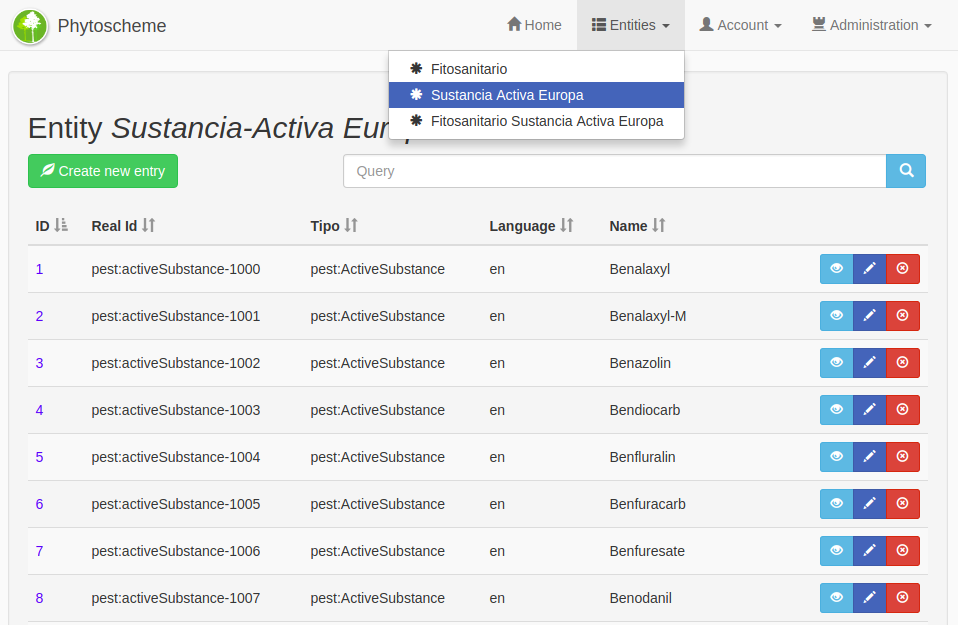
\includegraphics[width=\textwidth,height=\textheight,keepaspectratio]{Imagenes/capturaSustActivas}
    \caption{Captura de pantalla de la integración de las sustancias activas.}
    \label{fig:capturaSustActivas}
\end{figure}
\bigskip

\par 
\textbf{Tercera iteración para conseguir una integración y automatización completa - unión de los datos anteriores en una nueva tabla - Fitosanitario\_Sustancia\_Activa\_Europa}
\bigskip
\par 
Mientras que las dos primeras iteraciones se centraron en recoger datos periódicamente de fuentes independientes, subirlas a \textit{Hadoop} y luego importarlas en \textit{Hive} y \textit{MySQL} para ser consumidas por \textit{JHipster}, la tercera iteración tuvo que ver con la integración de dichas fuentes independientes dentro del sistema. Como se ha mencionado anteriormente, los datos de las sustancias activas europeas se eligieron como fuente para este proyecto dado que encajaban en cierta medida con los datos de los productos fitosanitarios autorizados en España:  Estos ultimos contienen un campo referente a las sustancias activas involucradas en el producto autorizado y gracias a eso se pudo hacer un \textit{mapping} entre ellos. No obstante, el \textit{mapping} no fue directo, puesto que los datos no venían en el mismo formato: en el caso de los productos autorizados, el campo en cuestión contenía además de los nombres de las sustancias activas en mayúscula la cantidad en la que podian estar presentes, mientras que en el caso de las sustancias activas europeas, los nombres venían en minúscula y sin la cantidad correspondiente. Así pues, en una primera aproximación lo que se hizo fue crear una tabla que contuviera los datos de los productos autorizados de España más una columna que fuera el identificador real de la \textbf{primera} sustancia activa involucrada en el producto. \par Esta aproximación no es la solución perfecta, no obstante, es una primera iteración que soluciona una parte del problema. Se consiguió gracias a una consulta en \textit{Hive} que partía los datos del campo \textit{formulado} (referente a las sustancias activas que forman el producto) de los productos autorizados de España, se quedaba con la primera cadena de sólamente literales y hacía el \textit{JOIN} con el nombre de la sustancia activa (pasado a mayúsculas) de la tabla de las sustancias activas europeas. 
\begin{figure}[!h]
    \centering
    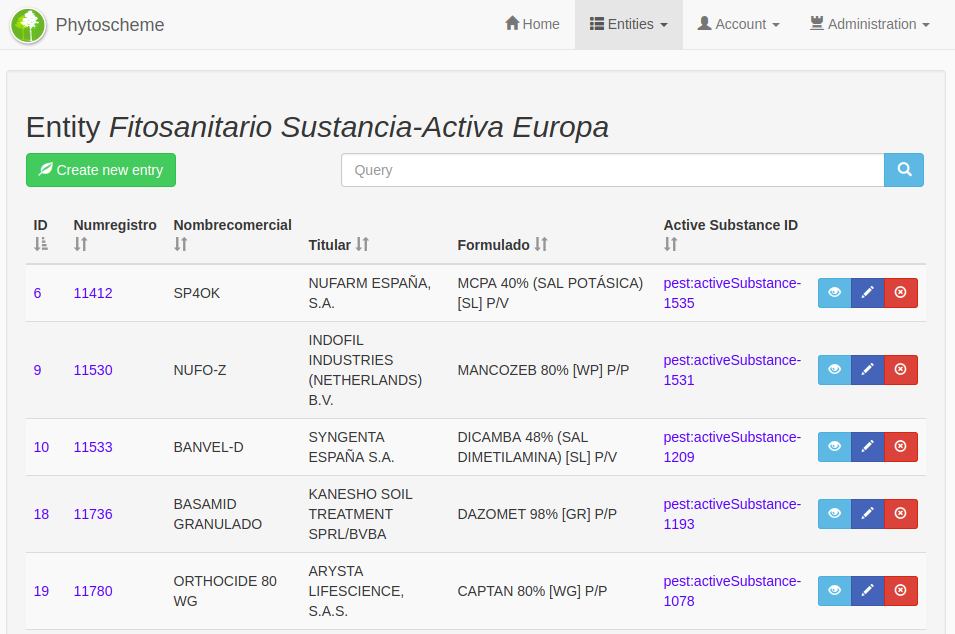
\includegraphics[width=\textwidth,height=\textheight,keepaspectratio]{Imagenes/capturaFitSustAct}
    \caption{Captura de pantalla de la integración de  los productos fitosanitarios y las sustancias activas.}
    \label{fig:capturaFitSustAct}
\end{figure}

\par Como primera solución provisional, se consigue hacer un \textit{matching} exitoso de unos cuatrocientos registros de un total de aproximadamente mil trescientas sustancias activas. En la figura \ref{fig:capturaFitSustAct} se puede observar el resultado de esta fase. No obstante, los problemas que presenta son los siguientes: 


\begin{itemize}
\item Hay productos autorizados que tienen mas de una sustancia activa como parte de su formulado y la consulta solo reconoce la primera de ellas.
\item Hay sustancias activas que aparecen en los productos autorizados de España que vienen en español y la consulta no es capaz de reconocerlos puesto que las sustancias activas de europa tienen su nomenclatura en inglés.
\end{itemize}


\bigskip

\par 
\textbf{Fichero de configuración}
\bigskip
\par
Para simplificar el acceso a los recursos se ha hecho uso de un fichero de configuración a los que acceden varios componentes: En primer lugar, el \textit{script bash} que descarga los datos de los productos autorizados del \textit{Mapama} \cite{mapama}. Este \textit{script} usa una función \textit{bash} para solicitar los valores del fichero de propiedades de la web del \textit{Mapama}, y saber la ruta en el sistema donde guardar dicho fichero. Si en cualquier momento se quiere modificar dicha localización, gracias al fichero de configuración, el único sitio que se debería modificar sería en el propio fichero. 
\par En segundo lugar, la aplicación \textit{Java} del \textit{Job} de \textit{Talend} también accede a dicho fichero de configuración, puesto que en él se han establecido tanto rutas de almacenamiento dentro del \textit{HDFS} de \textit{Hadoop}, como el nombre del nodo o del usuario. No obstante, tal como se ha comentado en el apartado anterior, esta aplicación \textit{Java} ha tenido que ser empaquetada en un archivo JAR único y conjunto con todas sus librerías. Entonces ... ¿cómo accede a dicho fichero de configuración?. La solución ha sido hacer que el \textit{archivo JAR} reciba la ruta a dicho fichero mediante un argumento, de forma robusta, tal que si no recibe argumentos, o si el fichero que se le pasa no es un fichero de propiedades, el proceso alerta del error y se detiene. 
\bigskip


\section{Problemas encontrados} \label{implementacion.problemas}
\par
Tal como se ha explicado a lo largo del desarrollo de esta memoria, tanto en la fase de la prueba de concepto como en la fase de desarrollo del prototipo se han encontrado diversos problemas de naturaleza técnica o tecnológica:

\paragraph*{Incertidumbre inicial.} El primero de los problemas que se detectaron tienen que ver con el arranque del proyecto. Debido a una incertidumbre inicial en cuanto a la estructura de su desarollo, en el arranque del proyecto no se pudo realizar una planificación inicial para dejar definida una visión global de toda su duración. Por ello surgieron problemas como que el alumno entendió que todo el trabajo de instalación y configuración de las herramientas sería una fase previa al desarrollo del proyecto en sí, lo cuál no fue asi, puesto que más tarde se establecería que dicho trabajo formaría parte de una primera fase del proyecto: la prueba de concepto. Además, dicha incertidumbre dificultó la gestión del proyecto: la definición de las tareas, el control de los esfuerzos y un análisis adecuado desde el principio.

\paragraph*{Sistema operativo.} Si bien es cierto que el sistema operativo donde se desarrollase el proyecto no era un requisito, apareció desde el principio como un derivado de las herramientas a utilizar. Se propuso un sistema operativo \textit{Linux} \cite{wikilinux} sobre el que llevar a cabo la implementación de la solución. 
La propia instalación del sistema resultó inicialmente problemática en el portátil del alumno debido a la inexistencia de los \textit{drivers} de \textit{Linux} necesarios para la tarjeta gráfica \textit{Nvidia} \cite{wikinvidia} presente en el equipo, que resultaba en el no arranque del sistema. Tras unos días de consultas y búsquedas en páginas y foros de Internet, la solución al problema fue añadir la instrucción \textit{nouveau.modeset=0}, que desactiva los drivers libres de \textit{Nvidia} en el menú \textit{GRUB}\footnote{GRUB - \url{https://www.gnu.org/software/grub/}} durante el arranque del sistema permitiendo que la gráfica que se ejecuta sea la otra presente en el equipo, la de \textit{Intel}.

\paragraph*{\textit{Hadoop}.} Como previamente se ha mencionado durante la prueba de concepto, la instalación de \textit{Hadoop} no fue la óptima desde el principio puesto que el alumno instaló una versión correspondiente a \textit{Ubuntu 14.04}, mientras que el sistema operativo instalado en el equipo era \textit{Ubuntu 16.04}. Debido a eso inicialmente \textit{Hadoop} dió problemas y en una fase posterior se tuvo que eliminar esta versión del equipo e instalar la correcta. Una vez solucionado ese problema, otro de los retos a los que se tuvo que enfrentar fue el entendimiento conceptual del sistema en sí. Se tuvieron que invertir horas en aprender a utilizar el sistema de ficheros \textit{HDFS}, algo necesario para el almacén de los datos de entrada de las diferentes fuentes. 
\par
Otro problema que surgió con \textit{Hadoop} fue debido a la falta de espacio en disco. Llegó un punto a lo largo de la duración del \textit{TFG} donde el disco duro del equipo del alumno se llenó y debido a eso las operaciones \gls{mapreduce} de \textit{Hadoop} se encolaban, se enmarcaban dentro de un estado de \textit{Pendiente} y nunca se ejecutaban. Pasaron varios días hasta que se llegó a la raíz del problema y, una vez liberada algo de memoria del disco duro, las operaciones \gls{mapreduce} de \textit{Hadoop} ya se podían realizar corréctamente. 

\paragraph*{\textit{Hive}.} Como ya se comentó, la instalación de \textit{Hive} en sí no presentó problemas. No obstante, el hecho de tratarse de un lenguaje \textit{SQL} nuevo, a pesar de su similitud con la sintáxis de \textit{MySQL} junto con las peculiaridades del sistema de archivos de \textit{Hadoop}, \textit{HDFS} sobre el que \textit{Hive} trabaja dificultaron un avance fluido del proyecto. En muchas ocasiones los datos de entrada daban problemas a la hora de importarlos en \textit{Hive}, por diferentes razones: inclusión de una cabecera que no debería aparecer en los datos de entrada, formateo incorrecto de los datos e incluso, por falta de experiencia, el uso incorrecto del delimitador en el lado de \textit{Hive}. Aparte de estas dificultades, \textit{Hive} también presentó problemas a la hora de intentar conectarlo diréctamente con \textit{JHipster}, tal como se verá en los siguientes apartados.

\paragraph*{Sqoop.} Al igual que \textit{Hive}, la instalación y configuración de \textit{Sqoop} no supuso un problema. No obstante, su manejo es lo que más dificultades presentó, puesto que al igual que los demás componentes, se trataba de una herramienta nueva para el alumno. Las tablas tanto de orígen (base de datos \textit{Hive} presente en \textit{HDFS}) como de destino (base de datos \textit{MySQL} de \textit{JHipster}) tenían que coincidir en estructura y tomó varios intentos hasta tener la configuración adecuada. 	

\paragraph*{\textit{JHipster}.} Con \textit{JHipster} se tuvo varios problemas, empezando por su instalación en el equipo. \textit{JHipster} utiliza \textit{Yarn}, \textit{Bower}, \textit{Node.js}, \textit{Gulp} y \textit{Yeoman} y, ya que el equipo tenía preinstaladas algunas de estas herramientas en sus antiguas versiones, al principio la instalación resultó en fallos que tomaron tiempo para solventar. Otro problema, una vez solucionado el anterior fue a la hora de la importación de una aplicación generada con \textit{JHipster} como proyecto dentro del entorno de desarrollo \textit{IntelliJ}. \textit{Gradle} inicialmente no estaba corréctamente configurado en el equipo y por ello el proyecto era incapaz de descargar y configurar sus dependencias. Tras haber instalado \textit{Graddle} e importado el proyecto corréctamente, otro de los problemas encontrados apareció a la hora de importar un esquema de datos sobre \textit{JHipster} mediante \textit{JDL-Studio}\footnote{JDL-Studio - \url{https://start.jhipster.tech/jdl-studio/}}, el editor gráfico para creación de modelos de datos de \textit{JHipster}. Si bien la creación del propio modelo y su descarga en un fichero  \textit{.jh} no presentó dificultades, la importación del esquema dentro del proyecto mediante el comando \textit{jhipster import-jdl fichero.jh} provocaba errores en el proyecto en el momento de su ejecución. Gracias al control de versiones implementado mediante \textit{GIT}\footnote{GIT - \url{https://git-scm.com}} se pudo volver a la versión previa y desechar los cambios provocados por el comando anterior. Se descubrió que si las entidades se crean individualmente mediante el comando \textit{jhipster entity nombreEntidad} el fallo anterior ya no ocurre y se puede continuar con una ejecución correcta. 
\par 
Otro problema con \textit{JHipster} ocurrió al intentar actualizar la versión del mismo. Según las instrucciones de la página web, el proceso debería ser aparentemente sencillo. Se trata de ir a la localización de la aplicación creada con \textit{JHipster} y ejecutar el comando \textit{jhipster upgrade}. No obstante, dicho comando en ocasiones funcionaba, y en otras, tras esperar el tiempo de actualización, todo aparentaba normalidad hasta que al arrancar la aplicación aparecían errores referentes a determinados \textit{beans} de \textit{Spring} que \textit{JHipster} era incapaz de encontrar. A pesar de intentar solucionar dicho problema, en esos casos el alumno prefirió volver a la versión anterior del proyecto y desechar los cambios realizados por el comando \textit{upgrade}. Como \textit{JHipster} es un sistema en constante evolución, periódicamente los desarrolladores lanzan \textit{parches} mediante los que solucionan problemas como el descrito anteriormente. 

\paragraph*{Integración de \textit{Hive} y \textit{JHipster}.} Tal como se explica en la prueba de concepto (sección \ref{implementacion.prueba}), inicialmente la arquitectura del sistema debía reflejar una conexión dirécta entre la aplicación de \textit{JHipster} y la base de datos \textit{Hive}, mediante la sustitución de la base de datos de \textit{JHipster} (\textit{MySQL}) por \textit{Hive} en los ficheros de configuración del proyecto. Teniendo en mente que \textit{JHipster} diréctamente \textbf{no ofrece soporte} ni para \textit{Hive} ni para \textit{Hadoop}, la meta era cambiar a nivel de código todos los parámetros y conexiones necesarias para \textit{engañar} a la aplicación y conseguir que trabaje diréctamente con \textit{Hive}. Esto consistía en importar las librerías necesarias, crear las entidades de \textit{JHipster} dentro de \textit{Hive}, indicarle el driver \textit{JDBC} para conectarse con \textit{Hive} y mapear cada acceso a la base de datos previa \textit{MySQL} a la de \textit{Hive}. El primer gran obstáculo que se detectó fue la importación de las librerías. Resulta que al importar las librerías necesarias para \textit{Hive}, estas presentaban conflictos con las librerías que ya venían importadas por \textit{JHipster}. Encontrar los paquetes conflictivos llevó mucho tiempo, puesto que el árbol de dependencias del proyecto tenía un tamaño considerable y no se podía saber a priori cuál de los múltiples duplicados existentes fallaba. Como se verá a continuación, el problema de las librerías externas dentro de \textit{JHipster} seguirá apareciéndo con otros componentes, por lo que se puede entender que \textit{JHipster} no es la mejor elección cuando se quiera expandir el proyecto con muchas librerías externas o de terceros. Por otro lado, el problema de las entidades se abordó poco a poco, intentando migrar las tablas una a una. No obstante, \textit{JHipster} creaba dichas tablas con una sintáxis y unas propiedades y atributos acordes a \textit{MySQL}, algunos de los cuales eran inviables de construir en \textit{Hive} debido a la misma inexistencia de dicha funcionalidad. Las aplicaciones que \textit{JHipster} generan tienen una gran complejidad, con cientas de clases interoperando y compartiendo información, dificultando la depuración de la ejecución del programa y haciendo que una aproximación como la que se intentaba realizar en este período fuera inviable. Tras semanas de intentos frustrados, se consiguió que la  aplicación arrancara conectándose a \textit{Hive}, pero era incapaz de realizar cualquier función que se le pedía, como iniciar sesión con un usuario o registrar uno nuevo así que la arquitectura del sistema cambió, se desechó la idea de conectar diréctamente \textit{Hive} con \textit{JHipster} y se abordó una aproximación que involucrara un intermediario (\textit{Apache Sqoop}) entre \textit{Hive} y \textit{JHipster} y manteniendo la base de datos \textit{MySQL}.

\paragraph*{\textit{Pentaho Kettle}.} Aparte del problema anterior, el otro gran obstáculo que supuso un retraso del proyecto fue la elección de \textit{Pentaho Kettle} como sistema para realizar operaciones \textit{ETL} sobre los datos previo a su importación en \textit{Hadoop}. Aparentemente \textit{Pentaho Kettle} era la herramienta que se buscaba complementaria al \textit{Stack Tecnológico} del proyecto. No obstante, con el tiempo se observó que más que una ayuda resultó un inconveniente. Desde su instalación, que resultó conflictiva puesto que por alguna razón al descargar el programa en español, este se descargó con la mitad de sus componentes en inglés y la otra mitad en español hasta su editor gráfico, que no es exáctamente muy \textit{user-friendly}. Se tuvo problemas para conectarse a \textit{Hadoop} ya que, por culpa de una documentación pobre no se da a entender que antes de intentar acceder a \textit{Hadoop} mediante sus componentes se debía configurar un \textit{Cluster} de \textit{Hadoop} dentro del propio editor gráfico. Además se observó que el lanzamiento de un mismo proceso varias veces podía resultar en una ejecución exitosa o fallar estrepitósamente por razones aparentemente arbitrarias. 

\paragraph*{\textit{Pentaho Kettle} y \textit{JHipster}.} A la hora de integrar \textit{Pentaho Kettle} y \textit{JHipster}, al igual que ocurría con \textit{Hive}, el problema principal fueron las librerías necesarias para poder trabajar con \textit{Pentaho Kettle} dentro de la aplicación de \textit{JHipster}. En este caso, además, reincidiéndo en el problema de la existencia de una documentación pobre, no se listan las librerías necesarias para poder trabajar con \textit{Pentaho Kettle} desde un proyecto \textit{Java}. Por esa misma razón, si bien es cierto que para trabajos o procesos sencillos (de prueba) de \textit{Pentaho Kettle} se consiguió el pack de librerías necesarias a importar, en cuanto los procesos eran un poco más complejos (como los que realmente necesitaba el proyecto), las librerías empezaban a producir conflictos en el proyecto, resultando en la imposibilidad del arranque de la aplicación. El problema fue que conforme se solucionaban los errores, aparecían otros, y cada vez en más cantidad, haciéndo inviable la opción de \textit{Pentaho Kettle} para los requisitos que tenía el proyecto. Por ello, tras reiterados intentos de solucionar dichos problemas se optó por buscar otras alternativas y se encontró \textit{Talend} como herramienta definitiva.

\paragraph*{\textit{Talend}.} El único problema que presentó \textit{Talend} realmente no supuso un retraso tan considerable. \textit{Talend} autogenera código \textit{Java} conforme el usuario diseña sus procesos en el editor gráfico. Resulta que uno de sus componentes (\textit{tHDFSInput}) en una primera instalación fallaba pues al insertar el código \textit{Java} correspondiente, se dejaba por cerrar una llave, haciéndo que el programa diese error en tiempo de compilación y no se pudiese probar el proceso. No obstante, tras reinstalar \textit{Talend}, este problema cesó y todos sus componentes funcionaron acordes a su especificación. 

\paragraph*{\textit{Talend} y \textit{JHipster}.} Reapareciéndo por tercera vez, el problema de las librerías importadas en \textit{JHipster} volvió a surgir al intentar integrar el código generado por \textit{Talend} de uno de sus procesos en el proyecto de \textit{JHipster}. Habiéndo aprendido la lección de los anteriores intentos, esta vez no se reparó mucho en intentar solventar este problema sino que se adoptó una solución alternativa: crear un proyecto \textit{Java} nuevo que integrase todas las dependencias necesarias para el proceso de \textit{Talend} y encapsular todo su contenido en una librería ejecutable, fácilmente accesible desde \textit{JHipster}. Esta solución también se probó con \textit{Pentaho Kettle}, pero como ya se mencionó, debido a la falta de documentación acerca de las librerías a importar, se desistió en su resolución.





























\chapter{Gestión} \label{gestion}
Este capítulo engloba aquellos aspectos que tienen que ver diréctamente con la gestión del proyecto: la metodología que se ha seguido a lo largo de todo su desarrollo, la  recogida de los esfuerzos y la organización del trabajo así como el control de versiones de los diferentes componentes del proyecto. Se reserva un apartado para mencionar las diferentes pautas e imposiciones que han afectado a un desarrollo libre del proyecto y  se recoge un estudio acerca de la estimación del coste del proyecto en sí. 

\section{Metodología} \label{gestion.metodologia}
Este apartado explica la metodología que se ha seguido para llevar a cabo el desarrollo del proyecto, desde su fase inicial llamada prueba de concepto (Sección \ref{implementacion.prueba}) hasta su finalización. Se podrían distinguir dos fases conceptuales acordes a los diferentes \textit{modus operandi} del desarrollo: 
\paragraph*{Prueba de concepto.} El desarrollo de la prueba de concepto ha sido guiado por el director del proyecto. Esto es, el director del proyecto marcó inicialmente el panorama global y el diseño que se quería seguir. A partir de allí, el trabajo consistió en instalar y configurar las herramientas propuestas por el director y validar su integración mediante un flujo de datos de prueba. Si tras un período de pruebas exhaustivas algún componente fallaba o no cumplía con los requisitos especificados en el análisis del proyecto, dicho componente era desechado y se buscaba una alternativa viable al mismo. Lo mismo ocurría si alguna conexión de integración concreta fallaba; por ejemplo, en el caso de intentar conectar \textit{Hive} con \textit{JHipster} diréctamente, al comprobar que era una solución inviable que no cumplía con los requisitos del proyecto se decidió que la alternativa sería mantener la base de datos original de \textit{JHipster} (\textit{MySQL}) y agregar un componente intermedio (\textit{Sqoop}) para la transferencia de los datos desde \textit{Hive} a \textit{MySQL}.
\paragraph*{Prototipo.} Una vez integradas las diferentes herramientas y elegido el \textit{stack tecnológico} final, la implementación del prototipo real se ha llevado a cabo mediante una metodología iterativa. Teniendo en mente que se trata de un proyecto con un potencial de crecimiento casi ilimitado, la aproximación más lógica fue agregar valor al proyecto mediante una aproximación de iteraciones agregativas, empezando por la integración de los productos fitosanitarios autorizados de España y siguiendo por los datos acerca sustancias activas de la base de datos Europea sobre pesticidas.  Así pues, en la primera iteración se diseñó e implementó el flujo capaz de descargar los datos acerca de los productos fitosanitarios autorizados de España de la fuente, almacenarlos en \textit{Hadoop}, transformarlos y prepararlos para su inserción en \textit{Hive}, su transferencia a \textit{MySQL} y su posterior visualización en \textit{JHipster}. En una segunda iteración se realizó lo mismo pero con los datos de las sustancias activas extraídos de la base de datos Europea de pesticidas. Siguiendo esta metodología y con el objetivo fijado en el crecimiento del proyecto se puede observar que los futuros avances del sistema se pueden realizar de la misma manera. Otro desarrollador podría retomar el trabajo en este punto y hacer que el programa siga creciendo mediante la expansión del número de iteraciones que agreguen nuevos flujos de datos para dar sporte a nuevas fuentes. La tercera iteración supuso la agregación del soporte capaz de mapear los datos de la primera iteración con los de la segunda, en una versión más que nada ilustrativa; a pesar de que dicha integración no es capaz de mapear el 100\% de los datos, esto no es un problema puesto que no era el objetivo perseguido. Lo que se perseguía era validar el modelo de integración y dar soporte a un crecimiento sencillo de la solución. Por último, siguiendo esta filosofía de iteraciones se agregó en una cuarta iteración un mecanismo para la detección de errores o inconsistencias en los datos integrados provenientes de diferentes fuentes. 

\section{Organización y control de versiones} \label{gestion.organizacion}
Otro área de la gestión del proyecto es su organización, a través de sus diferentes componentes. En este apartado se pretende dar una visión global de las estructuras y tecnologías involucradas en la organización del proyecto. 
\par En primer lugar, cabe mencionar que las diferentes herramientas que constituyen el \textit{core }tecnológico del proyecto (\textit{Hadoop}, \textit{Hive}, \textit{Sqoop}, \textit{JHipster}, \textit{Talend}, \textit{MySQL}) se han instalado sobre el equipo del alumno, en una partición local del disco duro. Esto proporcionó rapidez de despliegue y desarrollo para el alumno pero podría suponer dificultades a la hora de expandir el proyecto e incluso riesgos adicionales debido a una inexistencia de tolerancia a fallos o copias de seguridad. No obstante, tratándose de un \textit{TFG} se asumieron los riesgos y se adoptó esta postura como la más adecuada. 
\par En segundo lugar, la propia gestión de las tareas a desarrollar durante el proyecto se ha controlado mediante \textit{Trello}\footnote{Trello - \url{https://trello.com}} a través de un \textit{\gls{kanban}} de cuatro columnas (\textit{To do}, \textit{Doing}, \textit{Problem} y \textit{Done}): 
\begin{itemize}
\item La columna \textit{To do} almacena aquellas tareas que están pendientes de realizar o figuran como \textit{features} posibles a desarrollar.
\item La columna \textit{Doing} contiene aquellas tareas que el alumno desarrollaba en cada momento.
\item La columna \textit{Problem} sirve para almacenar aquellas tareas que presentan algún problema y dificultan su terminación. A través del mecanismo de comentarios de \textit{Trello} el alumno dejaba redactado el problema que ha tenido en dicha tarea para tener constancia de ello en todo momento y posteriormente poder arreglarlo. 
\item La columna \textit{Done} es donde se arrastraban todas las tareas que eran terminadas.
\end{itemize} 
En la figura \ref{fig:trello} se puede observar el tablero que el alumno ha usado a lo largo de casi toda la duración del proyecto.

\begin{figure}[!b]
    \centering
    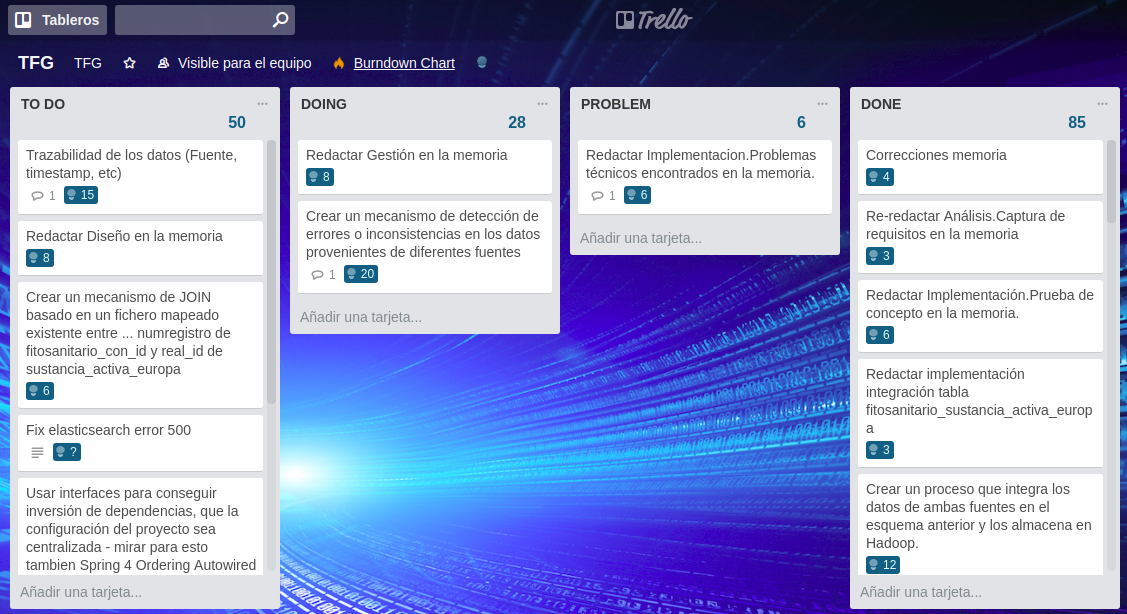
\includegraphics[width=\textwidth,height=\textheight,keepaspectratio]{Imagenes/trello}
    \caption{Tablero \textit{Trello} para la gestión de las tareas del proyecto.}
    \label{fig:trello}
\end{figure}

\par Otro aspecto de la organización se centra en la aplicación desarrollada con \textit{JHipster}. Inicialmente, esta se instaló al igual que las herramientas anteriores en el equipo local del alumno. No obstante, dado que sería una pieza fundamental y sobre la que se desarrollaría el software en sí, se decidió subirla a \textit{GIT} para mantener un control de versiones sobre ella. Profundizando más acerca de la organización del software desarrollado, dentro de la aplicación de \textit{JHipster} se creó un paquete encargado de mantener todo el código desarrollado por el alumno. Este paquete, llamado \textit{processes}, junto con sus subpaquetes y clases se puede observar en la figura \ref{fig:diag_clases}. Existe una clase principal llamada \textit{Schedule} encargada de lanzar los diferentes procesos. Aparte, se han designado distintos subpaquetes en función de las herramientas contra las que atacan: el paquete \textit{talend} es el que contiene los métodos encargados de ejecutar los trabajos desarrollados con \textit{Talend}. El paquete \textit{sqoop} contiene los métodos necesarios para poner en marcha una transferencia de \textit{Sqoop} desde \textit{Hive} a \textit{MySQL}. El paquete \textit{hive} contiene métodos que atacan contra la base de datos de \textit{Hive} mientras que el paquete \textit{mysql} contiene métodos que atacan contra la base de datos de \textit{MySQL}. El paquete \textit{common\_methods} es el único especial y contiene métodos públicos que puedan ser usados desde cualquiera de los demás paquetes. 
\par Como esta memoria también se quería mantener bajo un control de versiones riguroso, también se decidió que debería formar parte del software subido a \textit{GIT}. Así pues, en la carpeta raíz del proyecto de \textit{JHipster} se creó una carpeta llamada \textit{MEMORIA} donde se almacenaba todo lo referente a esta memoria.
\par Por último lugar, lo único restante de los diferentes componentes del proyecto son los diagramas desarrollados por el alumno tanto para el diseño de la aplicación como para los diferentes capítulos de la memoria y las hojas de gestión de esfuerzos. Estos componentes se crearon en \textit{Google Drive} y se han ido actualizando allí mismo. Dado que el alumno usa la aplicación web \textit{draw.io} para realizar los diagramas, esta aproximación se consideró como la más adecuada. 

\section{Control de esfuerzos} \label{gestion.esfuerzos}

En la primera fase del proyecto el alumno desconocía el panorama global del desarrollo del \textit{TFG}; desconocía el hecho de que habría dos fases, una en la que se realizaría una prueba de concepto y otra en la que se desarrollaría un prototipo real a partir de la validación de las herramientas empleadas en esa prueba de concepto; teniendo esto en mente, cabe destacar que el alumno consideró que el primer contacto con las herramientas, es decir, su instalación y configuración formarían parte de una fase previa, una especie de requisitos previos al arranque del proyecto, que no contabilizarían como esfuerzos en sí. Es por ello que al principio del proyecto el alumno no tomó nota de las horas precisas invertidas en aquella primera fase que más tarde se le revelaría que formaría parte de la prueba de concepto. No obstante, gracias a las herramientas como \textit{Drive} o \textit{Trello}, posteriormente se pudo hacer una recopilación aproximada de los esfuerzos invertidos durante esta fase. Así pues, una vez que se determinó la estructura final del proyecto se empezó a tener constancia de las horas a través de una hoja de cálculo almacenada en \textit{Drive} y gracias a ello se pueden presentar los esfuerzos divididos en las siguientes categorías: 
\begin{itemize}
\item \textbf{Análisis general. } La fase de análisis general comprendió un máximo de 30 horas aproximadas, entre la determinación de los requisitos, el análisis de los riesgos y la propia elección del \textit{Stack Tecnológico}. Aunque este último va diréctamente asociado a la prueba de concepto, cabe mencionarlo durante esta fase puesto que es donde a priori se analizaban las diferentes herramientas posibles de todo el elenco disponible. Además, en esta fase se incluye también el esfuerzo realizado por el alumno para comprender la problemática actual que se intenta resolver en este \textit{TFG}, desde lecturas de manuales fitosanitarios hasta portales web que explican los procesos actuales de importación y exportación de los mismos.
\item \textbf{Diseño general. } El diseño general del sistema tomó un máximo de 10 horas entre las diferentes variantes conceptuales; conforme se demostraba que un diseño aparente no cumplía con los requisitos del sistema, se procedía a diseñar otro, mejor adaptado a las necesidades del proyecto. 
\item \textbf{Prueba de concepto. } En las etapas anteriores se hablaba de un análisis y diseño generales. Esto es así dado que la prueba de concepto en sí incluye una parte de análisis y diseño como tal y se puede entender como separado de las fases previas. Además, al igual que las fases anteriores, gran parte de esta se ha desarrollado cuando aún no se tenía constancia precisa de las horas invertidas. No obstante, se pueden deducir alrededor de 90 horas totales que incluyen la instalación y configuración de las diferentes herramientas probadas junto con sus alternativas, las diferentes pruebas realizadas para conseguir un flujo de los datos desde su descarga hasta su transformación y presentación y la solventación de los diferentes errores que iban apareciéndo por el camino. 
\item \textbf{Implementación del prototipo. } La implementación del prototipo reune todos sus esfuerzos en la hoja de cálculo de \textit{Drive}, con un total de 66 horas de dedicación. En ellas están incluidos los diferentes procesos desarrollados en \textit{Talend}, los diferentes mecanismos para su integración en \textit{Java}, los \textit{crawlers} implementados en lenguaje \textit{bash} así como los  componentes software desarrollados en \textit{Java}. 
\item \textbf{Reuniones con el director del proyecto. } Se pueden deducir unas 18 horas de reuniones con el director del proyecto aunque este apartado se puede entender como algo más flexible que los anteriores, ya que, si bien es cierto que no han habido muchas reuniones planificadas con el profesor, este iba pasando por el laboratorio en el que el alumno desarrollaba el trabajo para revisar con él los avances conseguidos y apoyarle en la consecución de los objetivos. 
\item \textbf{Redacción de la memoria. } Las horas invertidas en la redacción de la memoria, al igual que en el bloque anterior, se recogen en su totalidad en la hoja de cálculo de \textit{Drive}. Han resultado un total de 110.5 horas.
\end{itemize}

En la figura \ref{fig:esfuerzos} se pueden observar las cifras anteriores en formato de diagrama de tarta. 

\begin{figure}[!h]
    \centering
    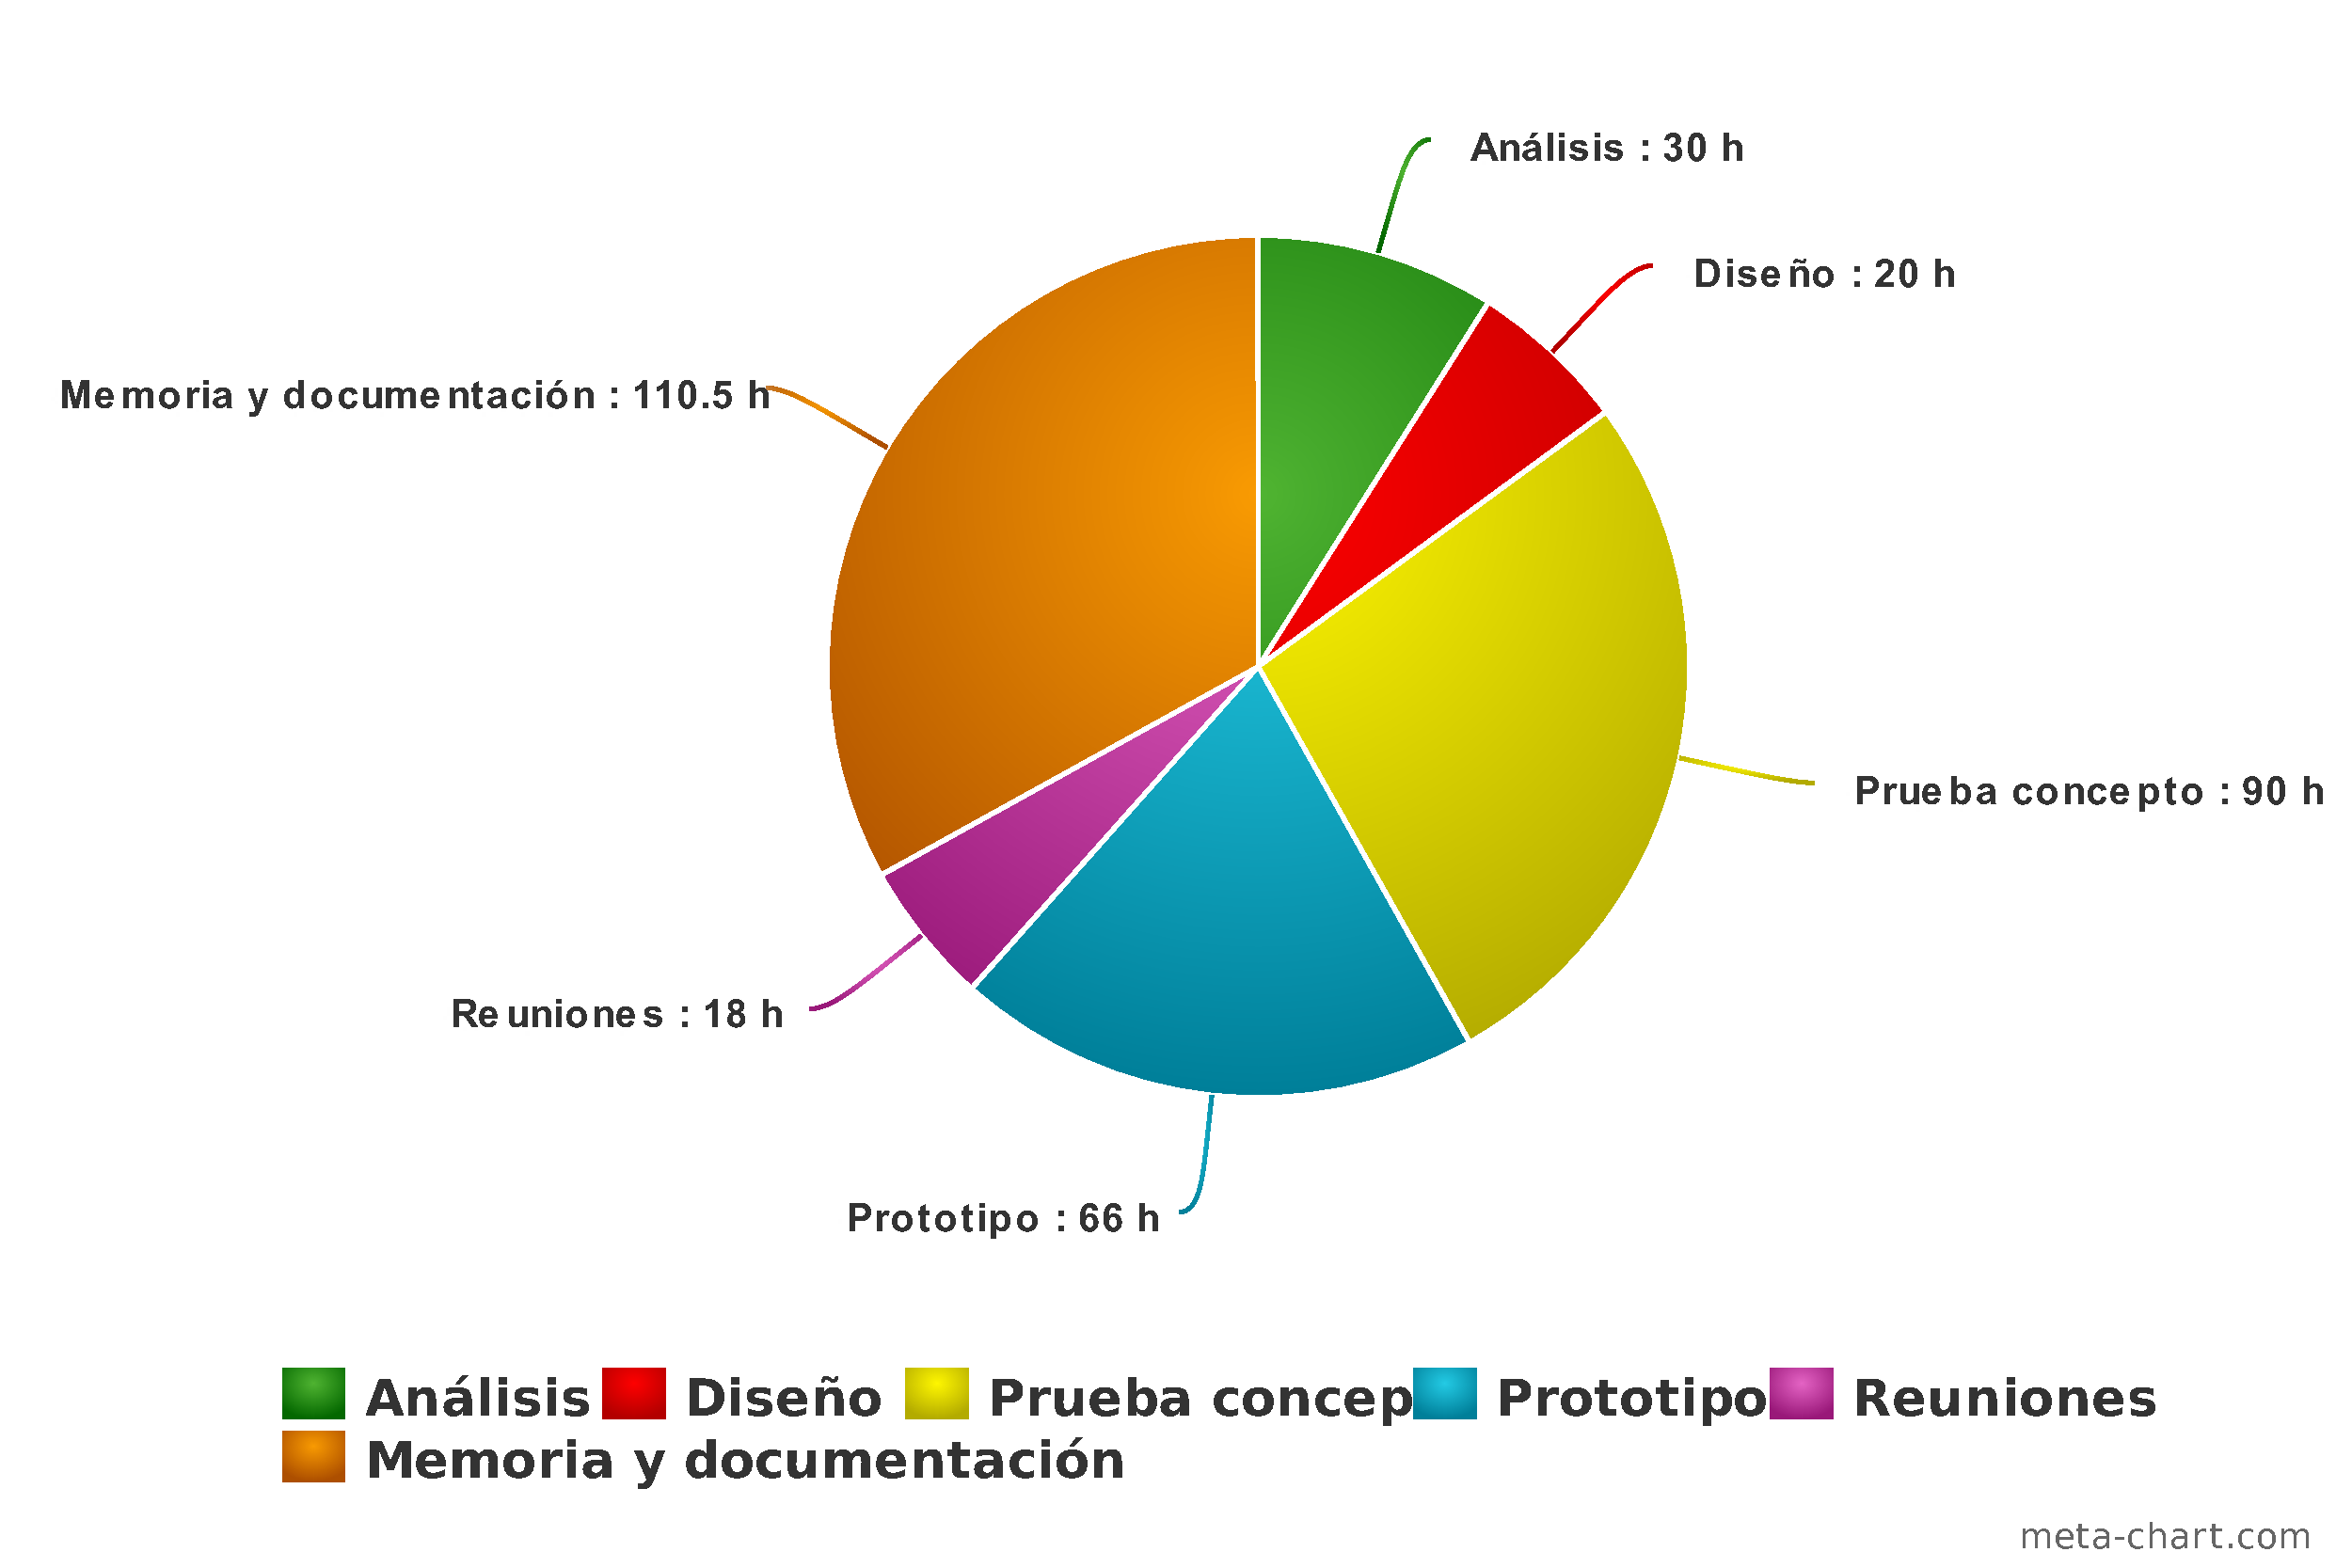
\includegraphics[width=\textwidth,height=\textheight,keepaspectratio]{Imagenes/esfuerzos}
    \caption{Horas de dedicación al proyecto.}
    \label{fig:esfuerzos}
\end{figure}


\section{Estimación del coste} 
\label{gestion.estimacion}

En este apartado se van a recoger los cálculos que se han llevado a cabo para calcular tanto el coste económico del \textit{TFG} como de la hora de trabajo de una persona que desarrollaría de manera comercial un proyecto como este. Para ello se ha hecho uso de la página web \textit{Calculadora Freelance} \cite{calculadorafreelance} y los resultados se pueden ver en los párrafos siguientes. 
\par 
Para calcular el coste económico del proyecto, se deben conocer a priori tanto las horas totales invertidas en el proyecto como el precio de la hora de trabajo del alumno; el resultado de la multiplicación de estos factores, sumado a otros elementos (como la gestión del proyecto, la gestión de configuraciones o el aseguramiento de la calidad), se corresponde al coste total del proyecto. Las horas invertidas en el proyecto han sido recogidas en el apartado anterior, mientras que la hora de trabajo del alumno se ha calculado a partir de los parámetros de la tabla \ref{tab:preciohora}.


\begin{table}[!h]
\centering
\bgroup
\def\arraystretch{1.3}
\begin{tabular}{l r}
\toprule
\textbf{Concepto} & \textbf{Cantidad} \\
 \midrule
 Sueldo esperado
& 
1500€ mensuales
 \\
 Días de vacaciones
& 
21 días anuales
 \\
 Días de inactividad
& 
7 días anuales
 \\
 Porcentaje reuniones, presupuestos, ventas, etc.
& 
50\%
 \\
 Gastos alquiler
& 
100€ mensuales
 \\
 Gastos en servicios (luz, móvil, etc.)
& 
50€ mensuales
 \\
 Impuesto autónomos
& 
260€ mensuales
 \\
 Otros gastos
& 
50€ mensuales
 \\
 Porcentaje beneficios
& 
20\%
\\
 \hline
 \textbf{TOTAL}
& 
\textbf{28.70€}
 \\
\bottomrule
\end{tabular}
\egroup
\caption{Precio por hora de trabajo}
\label{tab:preciohora}
\end{table}

Visto lo anterior, el coste mínimo de la hora de trabajo del alumno sería de \textbf{28.70€} y el desglose de los cálculos se puede observar en la sección \ref{d.gestion.estimacion} de los Anexos.

A continuación, en la tabla \ref{tab:costeproyecto} se recogen los diferentes componentes y tareas realizadas por el alumno junto con las horas dedicadas y el coste calculado, para conseguir el coste total del proyecto: 


\begin{table}[!h]
\centering
\bgroup
\def\arraystretch{1.3}
\begin{tabular}{l p{120pt} r}
\toprule
\textbf{Tarea/Componente} & \textbf{Horas} & \textbf{Coste (€)} \\
 \midrule
 Análisis general
& 
30 horas
& 
861.00€
 \\
 Diseño general
& 
20 horas
& 
574.00€
 \\
 Prueba de concepto
& 
90 horas
& 
2,583.00€
 \\
 Implementación prototipo
& 
66 horas
&
1,894.20€
 \\
 Reuniones
& 
18 horas
& 
516.60€
 \\
 Redacción Memoria
& 
110.5 horas
& 
3,171.35€
 \\
 \textbf{TOTAL Tareas/Componentes}
& 
\textbf{334.5 horas}
& 
\textbf{9,600.15€}
 \\
 \hline
 Gestión (G)
& 
334.5 h x 0.15
& 
1,440.02€
 \\
 Gestión de configuraciones (GC)
& 
334.5 h x 0.05
& 
480.01€
 \\
 Aseguramiento de la calidad (AC)
& 
334.5 h x 0.07
& 
672.01€
 \\
 \textbf{TOTAL GESTIÓN Y CALIDAD}
& 
\textbf{90.31 horas}
& 
\textbf{2,592.0405€}
 \\
 \hline
 Transporte (T)
& 
60 viajes x 2.70€
& 
162.00€
 \\
 \textbf{TOTAL MACROS}
& 
\textit{G+GC+AC+T}
& 
\textbf{2,754.04€}
 \\
 \hline
 Amortización estaciones de trabajo
& 
(334.5h + 90.31h) x \( \frac{800}{334.5 h} \)
& 
985.54€
 \\
 \textbf{TOTAL}
& 
& 
\textbf{13,339.73€}
 \\
\bottomrule
\end{tabular}
\egroup
\caption{Costes económicos del proyecto}
\label{tab:costeproyecto}
\end{table}
 
\chapter{Conclusiones}  \label{conclusiones}
\section{Resultados y objetivos} \label{conclusiones.resultados}
Se han conseguido los objetivos propuestos ? Están todos los requisitos cubiertos? Está bien documentada la solución? Es escalable ? …

\section{Conocimientos adquiridos} \label{conclusiones.conocimientos}
Resumir los conocimientos tanto a nivel personal como a nivel de tecnologías adquiridos.
 

 


%Puedes añadir más capítulos
%%%%%%%%%%%%%%%%%%%%%%%%%%%%%%%%%%%%%%%%%%%%%%%%%%%%%%%%%%%%%%%%%%%%%%%%%%%%%%%%%%%
%		BIBLIOGRAFÍA Y REFERENCIAS
%%%%%%%%%%%%%%%%%%%%%%%%%%%%%%%%%%%%%%%%%%%%%%%%%%%%%%%%%%%%%%%%%%%%%%%%%%%%%%%%%%%
\bibliographystyle{unsrt} %plaindin
\bibliography{Bibliografia_TFG}
\nocite{*} 

\printglossaries

\newpage
\renewcommand\listfigurename{Lista de Figuras}
\listoffigures

\newpage
\renewcommand\listtablename{Lista de Tablas}
\listoftables

%%%%%%%%%%%%%%%%%%%%%%%%%%%%%%%%%%%%%%%%%%%%%%%%%%%%%%%%%%%%%%%%%%%%%%%%%%%%%%%%%%%
%		ANEXOS
%%%%%%%%%%%%%%%%%%%%%%%%%%%%%%%%%%%%%%%%%%%%%%%%%%%%%%%%%%%%%%%%%%%%%%%%%%%%%%%%%%%

\newpage
\appendix
\clearpage
\addappheadtotoc
\appendixpage
\chapter{Datos} \label{a.datos}

\section{Esquema relacional de la base de datos \textit{JHipster}}


\begin{figure}[h!]
   
    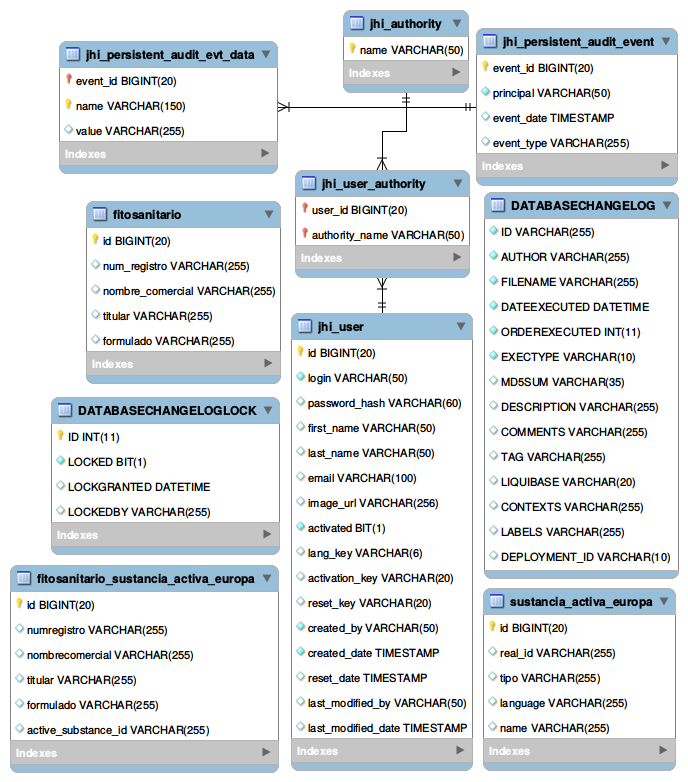
\includegraphics[width=\textwidth]{Imagenes/relational}
    \caption{Esquema relacional de la base de datos de \textit{JHipster}}
    \label{fig:relacionalmysql}
\end{figure}


\begin{landscape}
\section{Esquema de datos en la base de datos MySQL} \label{a.datos.modelo}
\begin{figure}[h!]
    
    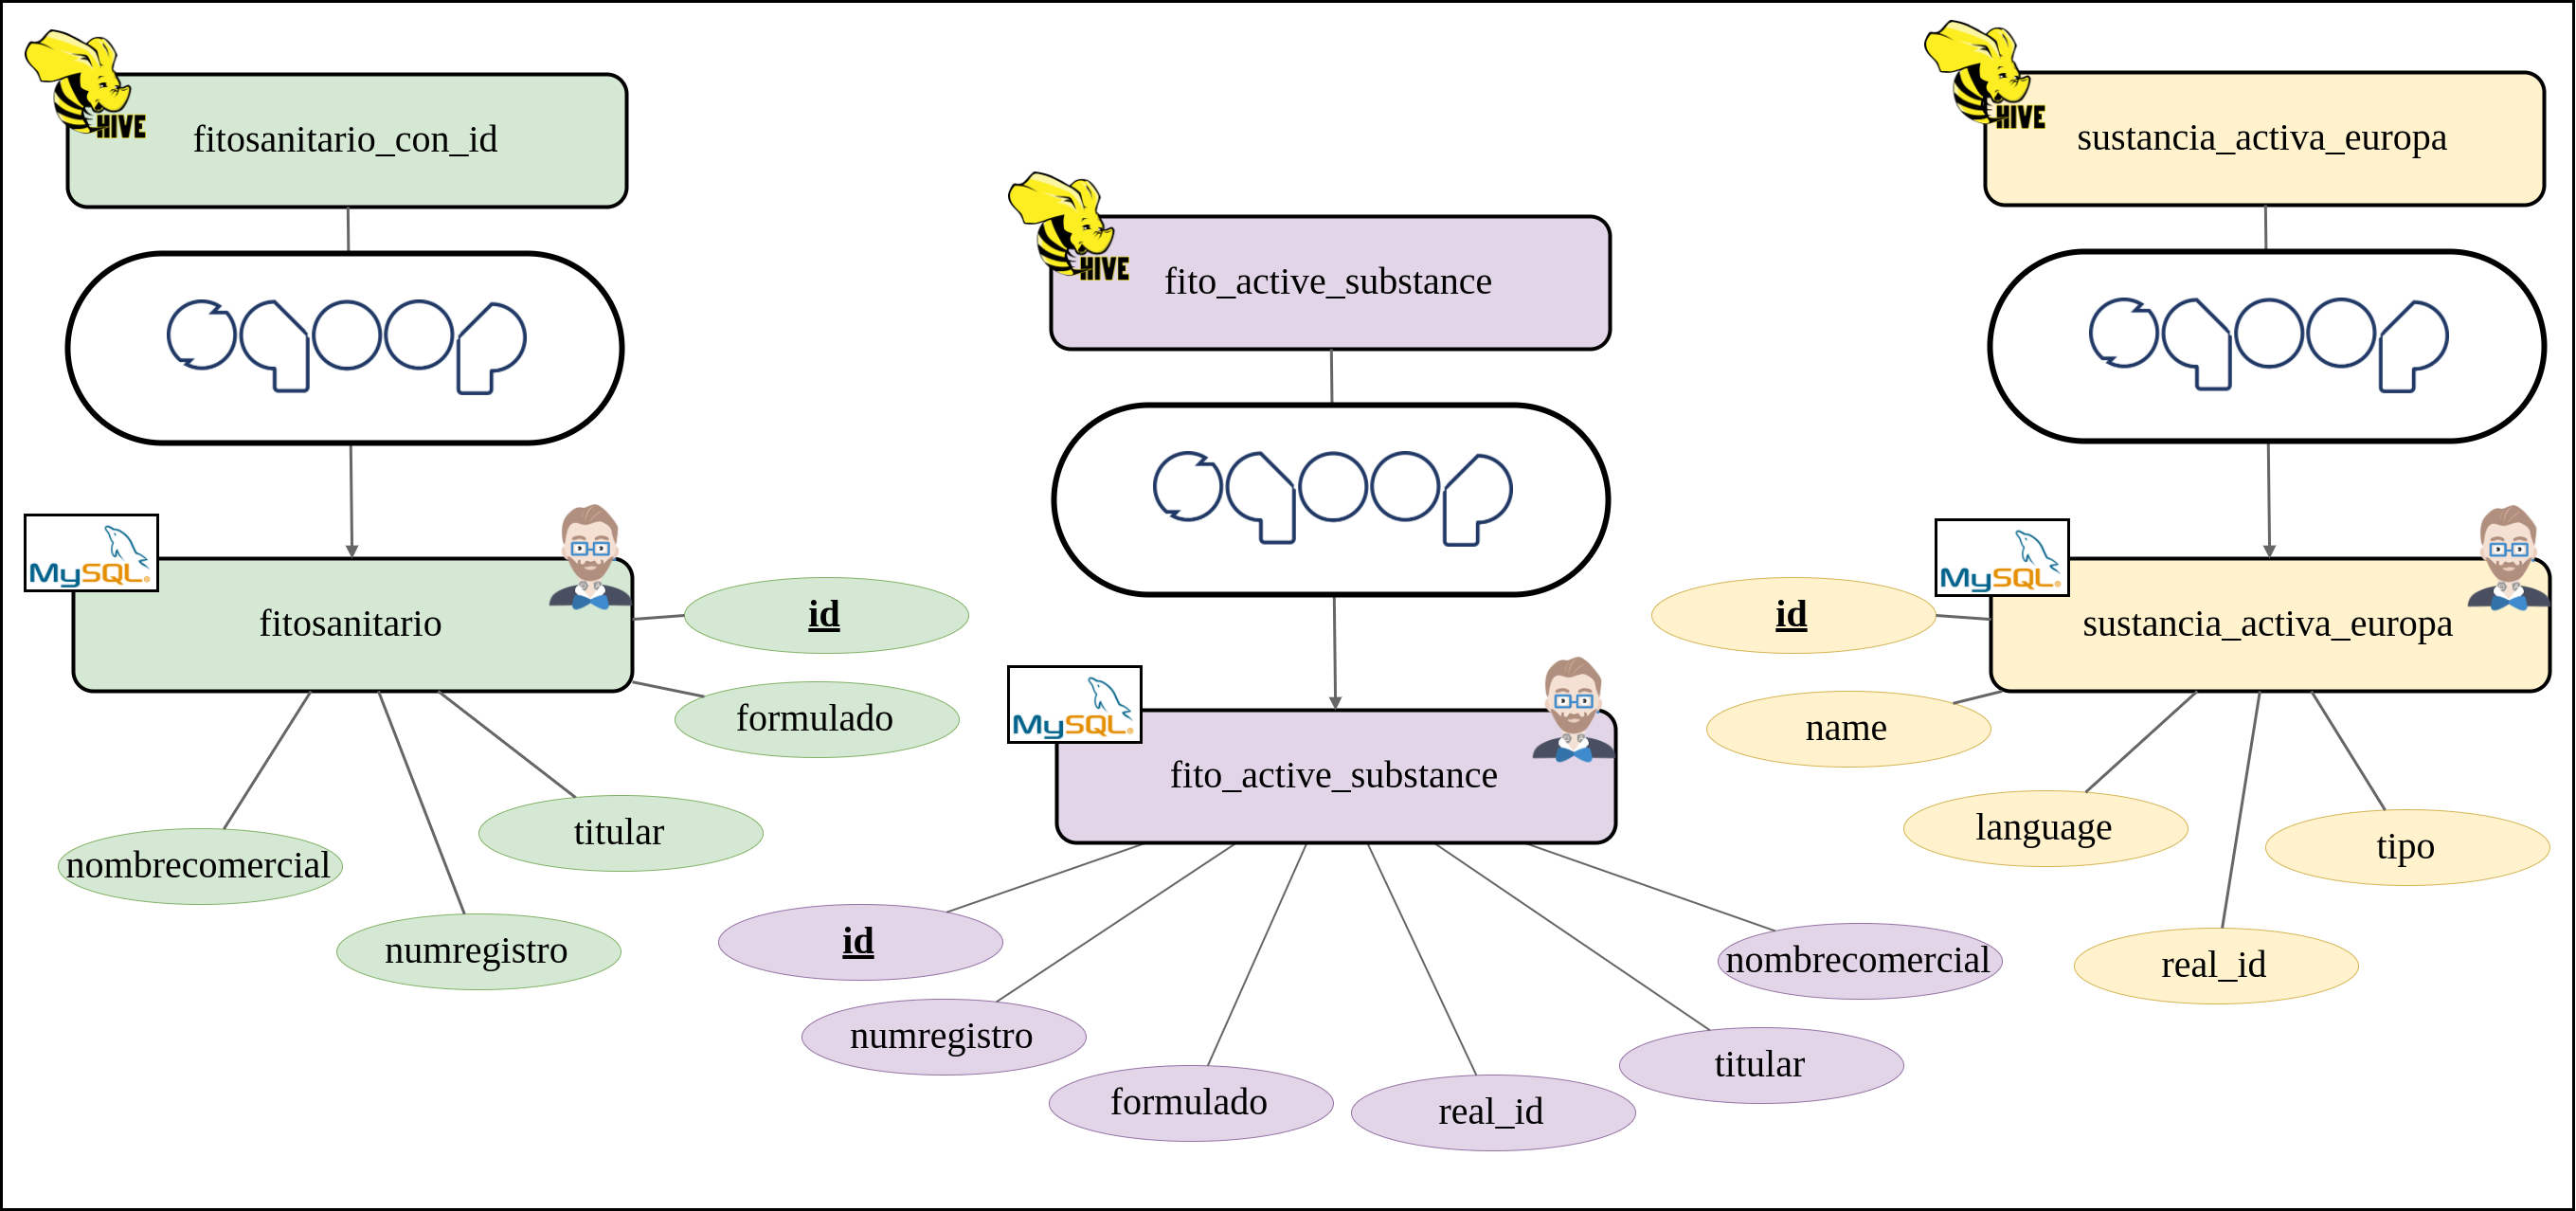
\includegraphics[width=1.5\textwidth]{Imagenes/datosmysql}
    \caption{Esquema de datos importados en \textit{MySQL} y \textit{JHipster}}
    \label{fig:datosmysql}
\end{figure}

\end{landscape}

\chapter{Análisis}
\section{Análisis de riesgos completos}
A continuación se exponen las diferentes fases del análisis de riesgos de manera detallada: 

\begin{enumerate}

\item \textbf{Identificación de los riesgos}

Se han intentado considerar el máximo número de riesgos y se han clasificado en diferentes categorías:

%FASE 1: Identificación de los riesgos
\begin{itemize}

\item \textbf{Riesgos globales}
\begingroup
\renewcommand\arraystretch{1.3}

\begin{longtable}{l p{5cm} p{9cm}}
% header and footer information
\hline
\textbf{ID} & \textbf{Nombre} & \textbf{Explicación} \\
\hline
\endhead
\endfoot
RG\_1 & 
Plazos &
El proyecto no se finaliza para la convocatoria de junio, septiembre o diciembre.
 \\
RG\_2 & 
Fallo del equipo &
El equipo principal de desarrollo falla, se pierde o estropea. 
 \\
RG\_3 & 
Incorporación mercado &
El alumno se incorpora al mercado laboral durante el desarrollo del proyecto, a falta de varios meses de su finalización.
 \\
RG\_4 & 
Experiencia del alumno &
El alumno no dispone de los conocimientos y preparación suficiente para el desarrollo del proyecto. 
 \\
\hline
\caption{Riesgos globales del proyecto}\label{ries_glob}\\
\end{longtable}

\item \textbf{Riesgos tecnológicos}
\begin{longtable}{l p{5cm} p{9cm}}
% header and footer information
\hline
\textbf{ID} & \textbf{Nombre} & \textbf{Explicación} \\
\hline
\endhead
\endfoot
RT\_1 & 
Tecnología nueva &
Se trata de una tecnología nueva.
 \\
RT\_2 & 
Software no probado &
Se debe interactuar con software que no ha sido probado. 
 \\
RT\_3 & 
Interfaz especializada &
Es requerida una interfaz de usuario especializada.
 \\
RT\_4 & 
Componentes diferentes &
Se necesitan componentes de programa diferentes a los hasta ahora desarrollados.
 \\
RT\_5 & 
Rendimiento &
Se necesitan componentes de programa diferentes a los hasta ahora desarrollados.
 \\
RT\_6 & 
Inalcanzable &
Se necesitan componentes de programa diferentes a los hasta ahora desarrollados.
 \\
\hline
\caption{Riesgos tecnológicos del proyecto}\label{ries_tecno}\\
\end{longtable}

\item \textbf{Riesgos de alcance}
\begin{longtable}{l p{5cm} p{9cm}}
% header and footer information
\hline
\textbf{ID} & \textbf{Nombre} & \textbf{Explicación} \\
\hline
\endhead
\endfoot
RA\_1 & 
Tamaño estimado &
Tamaño estimado del proyecto
 \\
RA\_2 & 
Confianza en la estimación &
Confianza en la estimación
 \\
RA\_3 & 
Número de elementos &
Número de programas, archivos y transacciones
 \\
RA\_4 & 
Tamaño almacenamiento &
Tamaño de las bases de datos involucradas
 \\
RA\_5 & 
Número de usuarios &
Número de usuarios 
 \\
RA\_6 & 
Número de cambios &
Número de cambios en los requisitos
 \\
RA\_7 & 
Software reutilizado &
Cantidad de software utilizado
 \\
\hline
\caption{Riesgos de alcance del proyecto}\label{ries_alcan}\\
\end{longtable}

\item \textbf{Riesgos de entorno de desarrollo}
\begin{longtable}{l p{5cm} p{9cm}}
% header and footer information
\hline
\textbf{ID} & \textbf{Nombre} & \textbf{Explicación} \\
\hline
\endhead
\endfoot
RE\_1 & 
Gestión proyectos &
Hay herramientas de gestor de proyectos
 \\
RE\_2 & 
Gestión proceso desarrollo &
Hay herramientas de gestión del proceso de desarrollo
 \\
RE\_3 & 
Análisis y diseño &
Se usan métodos y herramientas específicas para el análisis y diseño 
 \\
RE\_4 & 
Generadores de código &
Hay generadores de código apropiados para la aplicación
 \\
RE\_5 & 
Pruebas &
Hay herramientas de pruebas apropiadas
 \\
RE\_6 & 
Gestión de configuración &
Hay herramientas de gestión de configuración apropiadas
 \\
RE\_7 & 
Base de datos  &
Se hace uso de una base de datos o repositorio centralizado
 \\
RE\_8 & 
Integración &
Están todas las herramientas de desarrollo integradas
 \\
RE\_9 & 
Formación &
Se ha proporcionado formación a todos los miembros del equipo de desarrollo
 \\
RE\_10 & 
Expertos &
Hay expertos a los cuales solicitar ayuda acerca de las herramientas
 \\
RE\_11 & 
Ayuda online &
Hay ayuda en línea y documentación disponible
 \\
RE\_12 & 
Diseño arquitectónico &
Se utiliza un  método específico para el diseño arquitectónico y de datos
 \\
RE\_13 & 
Métricas de calidad &
Se disponen métricas de calidad para todos los proyectos de software
 \\
RE\_14 & 
Métricas de productividad &
Se disponen de métricas de productividad
\\
\hline
\caption{Riesgos de entorno de desarrollo del proyecto}\label{ries_entorno}\\
\end{longtable}

\endgroup

\end{itemize}

\item \textbf{Análisis del riesgo} \par

Para esta fase se han empleado los tres medidores del riesgo: la probabilidad, el impacto y la aceptación: 

%FASE 2: Análisis del riesgo - INTRODUCCION
\begin{itemize}

\item{\textbf{Tabla para estimar la probabilidad de un riesgo:}}
\begingroup
\renewcommand\arraystretch{1.3}
\begin{longtable}{l p{13cm}}
% header and footer information
\hline
\textbf{Valor} & \textbf{Descripción} \\
\hline
\endhead
\endfoot
Bajo (1) & 
La amenaza se materializa a lo sumo una vez cada año. 
 \\
Medio (2) & 
La amenaza se materializa a lo sumo una vez cada mes.
 \\
Alto (3) & 
La amenaza se materializa a lo sumo una vez cada semana.
 \\
\hline
\caption{Probabilidad de un riesgo}\label{prob_riesgo}\\
\end{longtable}

\item{\textbf{Tabla para estimar el impacto de un riesgo:}}
\begin{longtable}{l p{13cm}}
% header and footer information
\hline
\textbf{Valor} & \textbf{Descripción} \\
\hline
\endhead
\endfoot
Bajo (1) & 
El daño derivado de la materialización de la amenaza no tiene consecuencias relevantes para la consecución de los objetivos.  
 \\
Medio (2) & 
El daño derivado de la materialización de la amenaza tiene consecuencias reseñables para la consecución de los objetivos.
 \\
Alto (3) & 
El daño derivado de la materialización de la amenaza tiene consecuencias graves reseñables para la consecución de los objetivos.
 \\
\hline
\caption{Impacto de un riesgo}\label{impacto_riesgo}\\
\end{longtable}

\item{\textbf{Tabla para estimar la aceptación de un riesgo:}}


\begin{longtable}{l p{13cm}}
% header and footer information
\hline
\textbf{Valor} & \textbf{Descripción} \\
\hline
\endhead
\endfoot
Riesgo $\leq$ & 
La organización considera el riesgo poco reseñable. 
 \\
Riesgo $\geq$ 4 & 
La organización considera el riesgo reseñable y debe proceder a su tratamiento.
 \\
\hline
\caption{Aceptación de un riesgo}\label{aceptacion_riesgo}\\
\end{longtable}

\endgroup
\end{itemize}
\par La aceptación es una medida delimitadora que define aquellos riesgos que son considerados aceptables y aquellos ante los que se deben tomar medidas. Para esta medida se ha establecido un criterio de aceptación de 4. Cualquier riesgo cuyo valor sea menor que 4 se considera aceptable y por tanto un riesgo poco reseñable, mientras que aquellos que se encuentran por encima de 4 se consideran reseñables y se debe proceder a su tratamiento. 
\par
El cálculo de la gravedad del riesgo y su aceptación se realiza de la siguiente manera: se multiplica la probabilidad por el impacto, y si dicho valor excede el límite del criterio de aceptación, el riesgo se considera reseñable. 
A continuación, en base a las métricas anteriores, se especifican los riesgos de la fase 1 en las mismas categorías iniciales. Se resaltan en rojo aquellos riesgos cuya aceptación supera el 4.

%FASE 2: Análisis del riesgo - TABLAS
\begin{itemize}

\item \textbf{Riesgos globales}
\begingroup
\renewcommand\arraystretch{1.3}

\begin{longtable}{l p{5cm} ccc}
% header and footer information
\hline
\textbf{ID} & \textbf{Nombre} & \textbf{Probabilidad} & \textbf{Impacto} & \textbf{Riesgo} \\
\hline
\endhead
\endfoot
\textbf{RG\_1} & 
\textbf{Plazos} &
\textbf{2} &
\textbf{3} &
\textbf{6} 
 \\
RG\_2 & 
Fallo del equipo &
1 &
3 &
3 
 \\
RG\_3 & 
Incorporación mercado &
1 &
2 &
2 
 \\
RG\_4 & 
Experiencia del alumno &
2 &
2 &
4 
 \\
\hline
\caption{Valoración riesgos globales del proyecto}\label{ries_glob_valoracion}\\
\end{longtable}

\item \textbf{Riesgos tecnológicos}
\begin{longtable}{l p{5cm} ccc}
% header and footer information
\hline
\textbf{ID} & \textbf{Nombre} & \textbf{Probabilidad} & \textbf{Impacto} & \textbf{Riesgo} \\
\hline
\endhead
\endfoot
RT\_1 & 
Tecnología nueva &
3 &
1 &
3 
 \\
\textbf{RT\_2} & 
\textbf{Software no probado} &
\textbf{2} &
\textbf{3} &
\textbf{6} 
 \\
RT\_3 & 
Interfaz especializada &
1 &
1 &
1 
 \\
RT\_4 & 
Componentes diferentes &
3 &
1 &
3 
 \\
RT\_5 & 
Rendimiento &
2 &
2 &
4 
 \\
\textbf{RT\_6} & 
\textbf{Inalcanzable} &
\textbf{2} &
\textbf{3} &
\textbf{6} 
 \\
\hline
\caption{Valoración riesgos tecnológicos del proyecto}\label{ries_tecno_valoracion}\\
\end{longtable}

\item \textbf{Riesgos de alcance}
\begin{longtable}{l p{5cm} ccc}
% header and footer information
\hline
\textbf{ID} & \textbf{Nombre} & \textbf{Probabilidad} & \textbf{Impacto} & \textbf{Riesgo} \\
\hline
\endhead
\endfoot
\textbf{RA\_1} & 
\textbf{Tamaño estimado} &
\textbf{2} &
\textbf{3} &
\textbf{6} 
 \\
RA\_2 & 
Confianza en la estimación &
2 &
2 &
4 
 \\
\textbf{RA\_3} & 
\textbf{Número de elementos} &
\textbf{2} &
\textbf{3} &
\textbf{6} 
 \\
RA\_4 & 
Tamaño almacenamiento &
1 &
3 &
3 
 \\
RA\_5 & 
Número de usuarios &
1 &
3 &
3 
 \\
\textbf{RA\_6} & 
\textbf{Número de cambios} &
\textbf{2} &
\textbf{3} &
\textbf{6} 
 \\
RA\_7 & 
Software reutilizado &
1 &
1 &
1 
 \\
\hline
\caption{Riesgos de alcance del proyecto}\label{ries_alcan}\\
\end{longtable}

\item \textbf{Riesgos de entorno de desarrollo}
\begin{longtable}{l p{5cm} ccc}
% header and footer information
\hline
\textbf{ID} & \textbf{Nombre} & \textbf{Probabilidad} & \textbf{Impacto} & \textbf{Riesgo} \\
\hline
\endhead
\endfoot
RE\_1 & 
Gestión proyectos &
1 &
1 &
1 
 \\
RE\_2 & 
Gestión proceso desarrollo &
1 &
1 &
1 
 \\
RE\_3 & 
Análisis y diseño &
1 &
2 &
2 
 \\
RE\_4 & 
Generadores de código &
1 &
1 &
1 
 \\
RE\_5 & 
Pruebas &
2 &
2 &
4 
 \\
RE\_6 & 
Gestión de configuración &
2 &
2 &
4 
 \\
RE\_7 & 
Base de datos  &
1 &
3 &
3 
 \\
RE\_8 & 
Integración &
1 &
1 &
1 
 \\
\textbf{RE\_9} & 
\textbf{Formación} &
\textbf{2} &
\textbf{3} &
\textbf{6} 
 \\
RE\_10 & 
Expertos &
2 &
1 &
2 
 \\
RE\_11 & 
Ayuda online &
2 &
2 &
4 
 \\
RE\_12 & 
Diseño arquitectónico &
2 &
1 &
2 
 \\
RE\_13 & 
Métricas de calidad &
3 &
1 &
3 
 \\
RE\_14 & 
Métricas de productividad &
3 &
1 &
3 
\\
\hline
\caption{Valoración de los riesgos de entorno de desarrollo del proyecto}\label{ries_entorno_valoracion}\\
\end{longtable}

\endgroup

\end{itemize}

\item \textbf{Priorización de riesgos} \par
Esta fase incluye todos los riesgos, ordenados de mayor a menor severidad. Se resaltan en rojo los riesgos que habrá que considerar en un plan de defensa estratégico posterior:


\begingroup
\renewcommand\arraystretch{1.3}

\begin{longtable}{l p{5cm} c}
% header and footer information
\hline
\textbf{ID} & \textbf{Nombre} & \textbf{Riesgo} \\
\hline
\endhead
\endfoot
\textbf{RG\_1} & 
\textbf{Plazos} &
\textbf{6} 
 \\
\textbf{RT\_2} & 
\textbf{Software no probado} &
\textbf{6} 
 \\
\textbf{RT\_6} & 
\textbf{Inalcanzable} &
\textbf{6} 
 \\
\textbf{RA\_1} & 
\textbf{Tamaño estimado} &
\textbf{6} 
 \\
\textbf{RA\_6} & 
\textbf{Número de cambios} &
\textbf{6} 
 \\
\textbf{RE\_9} & 
\textbf{Formación} &
\textbf{6} 
 \\
 
RT\_5 & 
Rendimiento &
4 
 \\
RA\_2 & 
Confianza en la estimación &
4 
 \\
RE\_5 & 
Pruebas &
4 
 \\
RE\_11 & 
Ayuda online &
4 
 \\
RG\_2 & 
Fallo del equipo &
3 
 \\
RT\_1 & 
Tecnología nueva &
3 
 \\
RT\_4 & 
Componentes diferentes &
3 
 \\
RA\_4 & 
Tamaño almacenamiento &
3 
 \\
RA\_5 & 
Número de usuarios &
3 
 \\
RE\_7 & 
Base de datos &
3 
 \\
RE\_13 & 
Métricas de calidad &
3 
 \\
RE\_14 & 
Métricas de productividad &
3 
 \\
RG\_3 & 
Incorporación mercado &
2 
 \\
RE\_3 & 
Análisis y diseño &
2 
 \\
RE\_10 & 
Expertos &
2 
 \\
RE\_12 & 
Diseño arquitectónico &
2 
 \\
RT\_3 & 
Interfaz especializada &
1 
 \\
RT\_7 & 
Software reutilizado &
1 
 \\
RE\_1 & 
Gestión proyectos &
1 
 \\
RE\_2 & 
Gestión proceso desarrollo &
1 
 \\
RE\_4 & 
Generadores de código &
1 
 \\
RE\_8 & 
Integración &
1 
 \\
\hline
\caption{Priorización de riesgos del proyecto}\label{prioriz_riesg}\\
\end{longtable}

\endgroup
Como se puede apreciar, hay 6 riesgos cuyo factor de gravedad es preocupante y deben ser tratados acordemente: 
\begin{enumerate}
\item RG\_1. Riesgo global “Plazos”. Tiene que ver con el hecho de no acabar el proyecto dentro de los plazos establecidos para su defensa. Hay 2 fechas recomendables para su defensa, la primera en Junio de 2017 y la segunda en Septiembre de 2017. No obstante, se dispone de otra oportunidad en Diciembre de 2017, aunque sería la menos recomendable dado que supondría el retraso de la defensa y con ello la dificultad del estudiante de realizar otras actividades mientras tanto. A partir de Diciembre, la consecuencia sería volver a matricularse en el proyecto y aportar las tasas de la matrícula por segunda vez.
\item RT\_2. Riesgo de tecnologías “Software no probado”. Tiene que ver con la probabilidad de usar en el proyecto software que previamente no ha sido probado y pueda fallar. Obtuvo una valoración de gravedad de 6/6 puesto que si bien es cierto que todas las tecnologías han sido probadas individualmente y se sabe que funcionan bien, el proceso en su conjunto no ha sido probado. No se sabe si es viable o no.  
\item RT\_6. Riesgo de tecnologías “Inalcanzable”. Relacionado con el hecho de que el proyecto puede tener como conclusión un resultado negativo; Al tratarse de un trabajo de investigación, el resultado puede ser que no se ha logrado la integración deseada.
\item RA\_1. Riesgo de alcance “Tamaño estimado”. Tiene que ver con el hecho de que el proyecto resulte mucho más grande de lo estimado inicialmente, y por diferentes circunstancias no se llegue a finalizar.
\item RA\_6. Riesgo de alcance “Número de cambios”. Otro riesgo es el hecho de que los requisitos cambien constantemente, bien porque los clientes lo solicitan bien porque las propias tecnologías lo imponen. 
\item RE\_9. Riesgo de entorno de desarrollo “Formación”. Este riesgo trata con el hecho de que el alumno disponga de la formación necesaria y suficiente para lograr los objetivos propuestos.
\end{enumerate}

\item \textbf{Planificación de la gestión de riesgos} \par
En esta fase se recogen las conclusiones mitigadoras acerca de los riesgos "preocupantes" del proyecto, en relación a su factor de gravedad: 

\begin{enumerate}
\item RG\_1: Plazos - Como medida mitigante, el alumno deberá dedicar un horario de jornada completa a la realización del proyecto durante el verano del año 2017. 
\item RT\_2: Software no probado - La contrapartida y defensa de este riesgo es desarrollar o experimentar primero con una prueba de concepto para validar que las tecnologías en su conjunto funcionen correctamente. 
\item RT\_6: Inalcanzable - La mitigación este riesgo está ligada al anterior. Por lo tanto, primero se hará una prueba de concepto para demostrar si las tecnologías empleadas se pueden usar en conjunto.
\item RA\_1: Tamaño estimado - La solución desde un principio debe definir bien el alcance y determinar aquellas cosas que formarán parte de la solución y aquellas que no lo harán. 
\item RA\_6: Número de cambios - El alumno y el profesor deben acordar al principio unos requisitos fijos que no podrán ser modificables, en conjunto con el hecho de definir claramente el alcance de la solución.
\item RE\_9: Formación - Para mitigar este riesgo, el alumno debe estar en constante aprendizaje, utilizando los manuales y tutoriales de las diferentes herramientas de las que va a hacer uso durante el proyecto. Además, el alumno tendrá a su disposición al director del proyecto para consultar dudas y a los diferentes foros tecnológicos de Internet. 
\end{enumerate}
\end{enumerate}

\section{Análisis de diseños alternativos}

Al igual que los requisitos, el diseño de la solución también ha sufrido constantes cambios. Inicialmente la propuesta de trazabilidad de la solución es la que se puede observar en la figura 1. \par

\begin{figure}[H]
    \centering
    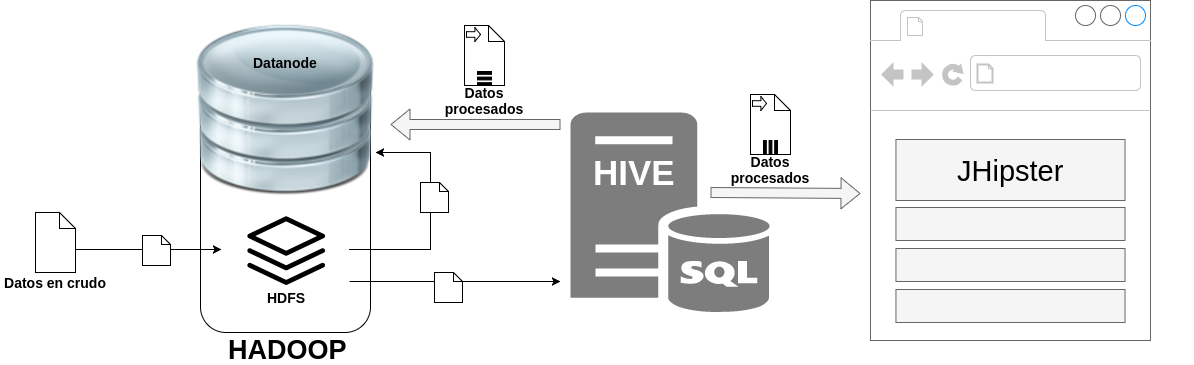
\includegraphics[width=1\textwidth,height=5.5cm]{Imagenes/Dis_Fig_1}
    \caption{Diseño primitivo del sistema.}
    \label{fig:dis_1_sist}
\end{figure}
\par


Como se puede observar, inicialmente el concepto giraba alrededor de las tres tecnologías core: Hadoop, Hive y JHipster. No se tuvo en consideración otras herramientas puesto que se pensaba que era suficiente para resolver el problema. Los datos en crudo, extraídos de la web del magrama o de otras fuentes heterogéneas, serían almacenados en Hadoop, en un nodo local mediante el sistema de ficheros HDFS, y posteriormente sería HIVE el encargado de procesarlos en su totalidad hasta conseguir almacenarlos en un esquema común. Además, la misma “base de datos” de Hive funcionaría como base de datos para la aplicación desarrollada con JHipster, sirviendo en todo momento ese esquema único para la visualización del mismo en un navegador web. Este diseño, conceptualmente fue la solución ideal para el problema planteado; no obstante, debido a que JHipster no ofrece soporte para cambiar la base de datos con la que se construye la aplicación y mucho menos soporte para Hive o Hadoop, tras muchos intentos frustrados de conseguir esta conectividad directa, se optó por una solución diferente, alejada de este diseño ideal pero rebelde, en contra de los paradigmas de programación que JHipster impone. La alternativa a este diseño que dió resultados y eliminó complicaciones fue la que se observa en la figura 2. \par


\begin{figure}[H]
    \centering
    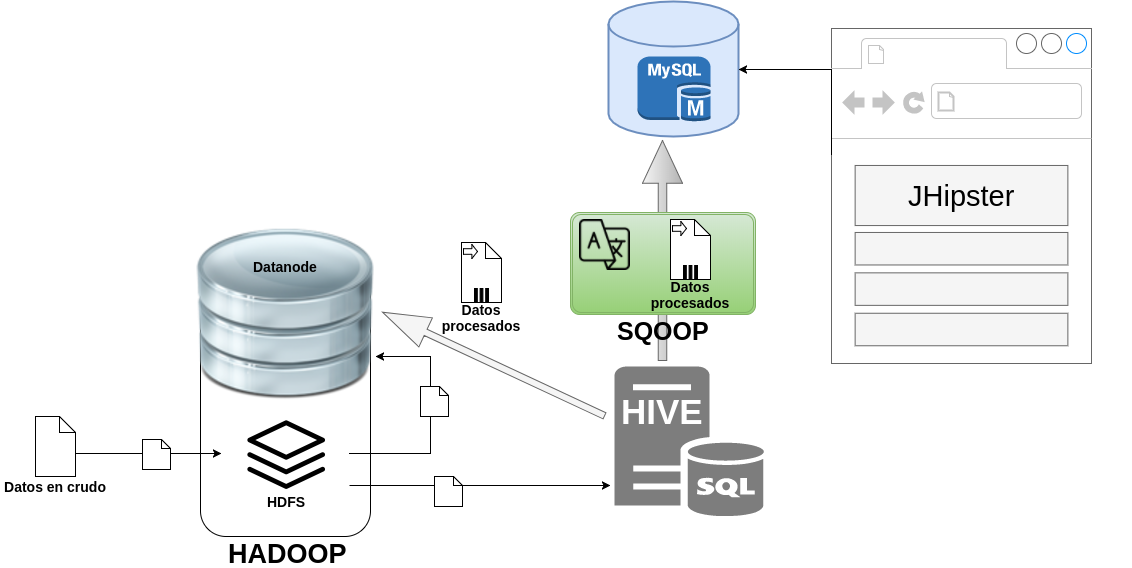
\includegraphics[width=1\textwidth,height=8cm]{Imagenes/Dis_Fig_2}
    \caption{Segunda iteración del diseño del sistema.}
    \label{fig:dis_2_sist}
\end{figure}
\par


En la segunda fase del diseño, se observa la evolución de la idea, condicionada por los problemas anteriormente mencionados. En primer lugar, se conservó la base de datos nativa de JHipster, en este caso una base de datos MySQL convencional. En ella se almacenaria únicamente la estructura final del esquema unificado, con los datos finales. Dichos datos tendrían que ser pasados desde Hive mediante una herramienta de transformación y transporte de datos. En este caso se usó Sqoop, una herramienta gratuita que permite transportar los datos desde Hive a MySQL, puesto que ofrece soporte tanto para Hadoop, HDFS y Hive como para MySQL. \par
Una vez resuelto el problema de la visualización de los datos, lo próximo que se detectó fue esa necesidad de procesamiento de los datos en crudo antes de incluso exponerlos como un esquema relacional en Hive. Para eso, lo mejor era hacer uso de algún programa de procesado de ficheros y una de las mejores opciones aparentes era Pentaho, un programa completo de transformación de ficheros. Pentaho venía con soporte para Hadoop y HDFS, por lo que gracias a eso se pudo trabajar con ficheros directamente extraídos de Hadoop, y almacenarlos directamente en Hadoop. Los cambios se pueden observar en la figura 3. \par


\begin{figure}[H]
    \centering
    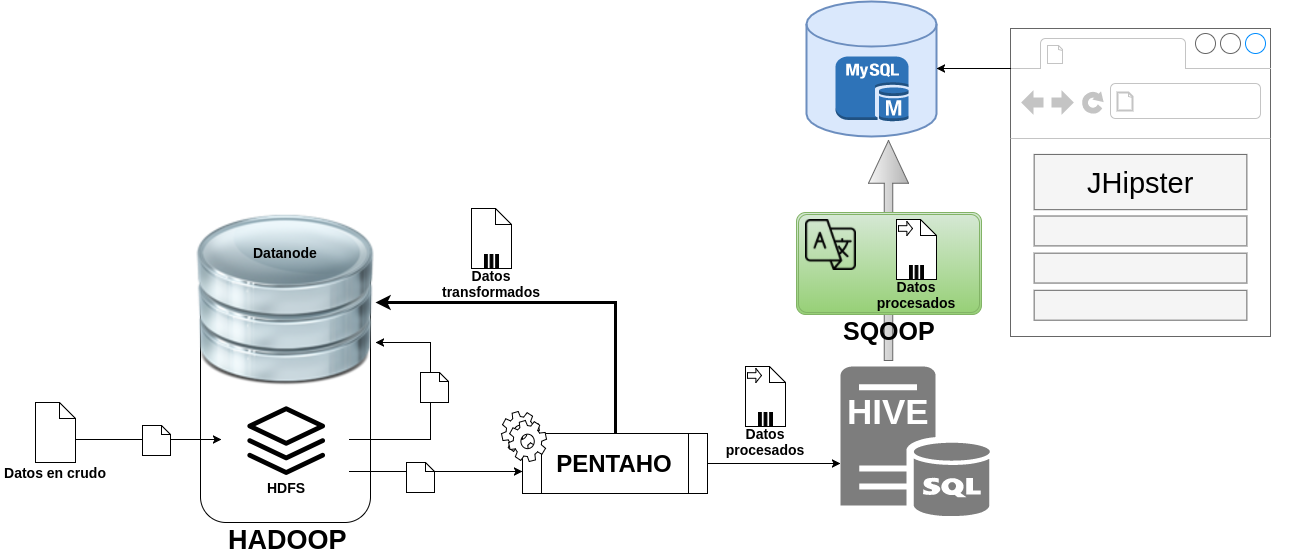
\includegraphics[width=1\textwidth,height=7cm]{Imagenes/Dis_Fig_3}
    \caption{Tercera iteración del diseño del sistema.}
    \label{fig:dis_2_sist}
\end{figure}
\par


INACABADO


\chapter{Diseño} 
\label{e.disenyo}
\section{Prueba de concepto en detalle} 
\label{e.disenyo.pruebaconcepto}
A continuación se van a presentar detalladamente las herramientas usadas y las pruebas realizadas durante el desarrollo de la prueba de concepto. Además, se van a exponer algunos de los retos enfrentados durante la duración de la misma y la manera en la que se han ido solucionando. Una visión gráfica y temporal del desarrollo de la prueba de concepto se puede observar en la figura \ref{fig:pruebaconceptoglobal}. 

\par
\paragraph*{Hadoop.}

\par
Inicialmente la instalación de \textit{Hadoop} supuso algunos problemas puesto que el alumno no había tenido contacto con la herramienta previamente, y la \textit{información} \cite{hadoop_installation_bad} que el alumno seleccionó como base para la instalación estaba desafortunadamente incorrecta (la instalación disponible en dicha web había sido probada con \textit{Ubuntu Linux 10.04}, pero no con la versión del alumno, la \textit{16.04}). Por lo tanto, se tuvo que empezar de cero, eliminando cualquier rastro de la primera instalación de \textit{Hadoop} del sistema. Después de ello, en un segundo intento, y gracias al \textit{tutorial de instalación de Hadoop de Digital Ocean} \cite{hadoop_installation} el programa funcionó correctamente y se procedió a instalar el siguiente bloque software necesario para el funcionamiento del sistema: \textit{Hive}.


\par
\paragraph*{Hive.}

\par
Para la instalación de \textit{Hive} ocurrió un problema similar al de \textit{Hadoop}. La fuente elegida para su instalación no fue la adecuada en un principio; el alumno eligió el tutorial expuesto en la web \textit{Tutorial's Point} \cite{hivetutorialspoint}, que provee información no solo excesiva sino en ocasiones confusa. Como en el caso anterior, se tuvo que erradicar \textit{Hive} del sistema para proceder con una instalación más limpia, esta vez desde la \textit{página web oficial de Hive} \cite{hive_installation}, puesto que lo único requerido para su instalación fue su descarga y la declaración de las variables de entorno necesarias para su ejecución. De esta manera, se consiguió instalar la versión 2.2.1 de \textit{Hive} sin dificultades. 


\par
\paragraph*{JHipster: Instalación.}

\par
Lo siguiente que se probó fue a instalar \textit{JHipster}. Como \textit{Java} y \textit{Node.js}\footnote{Node.js \textregistered - \url{https://nodejs.org/en/}}, dos de los componentes necesarios para su instalación ya estaban configurados en el equipo, lo único que se tuvo que configurar fue \textit{Yarn}, que se hizo siguiendo los pasos recomendados para \textit{Linux} en la \textit{página oficial de Yarn} \cite{yarninstall} para poder instalar \textit{JHipster} con el comando \textit{yarn global add generator-jhipster}, tal como indica la página oficial de \textit{JHipster}. Esto en sí fue facil, y no supuso mayor problema; No obstante, el desconocimiento de \textit{Yarn} junto con las actualizaciones periódicas que se introducían en \textit{JHipster} hicieron que más de una vez se tuviese que borrar \textit{JHipster} del equipo y volver a instalarlo en su última versión.  


\par
\paragraph*{JHipster: Aplicación de prueba.}

\par
Con \textit{JHipster} instalado y configurado en el sistema, el siguiente paso obvio fue crear una aplicación y verla en funcionamiento. Para ello se siguió el tutorial del que se provee en la \textit{página oficial}. La creación de la aplicación con JHipster resultó bastante sencillo puesto que se trata de pasos secuenciales. No obstante, dado que en la web no existe mucha información acerca de la integración de un proyecto  \textit{JHipster} con \textit{IntelliJ}\footnote{IntelliJ IDEA - \url{https://www.jetbrains.com/idea/}} (entorno de desarrollo usado por el alumno), el arranque resultó bastante frustrante. El poco dominio que el alumno tenía tanto de \textit{Gradle} como del propio entorno supuso un reto en las fases tempranas del proyecto, que se superó a base de leer documentación y realizar diversos intentos hasta que por fin se consiguió una versión de la aplicación corriendo en local, en el puerto 8080. 


\par
\paragraph*{Integración Hadoop - Hive - JHipster.}

\par
Si bien es cierto que la integración entre \textit{Hive} y \textit{Hadoop} resulta casi trivial, la integración entre \textit{Hive} y \textit{JHipster} es todo lo contrario. En primer lugar, se quería conectar \textit{Hive} con \textit{Hadoop} para disponer de una ayuda relacional para poder hacer consultas sobre datos en formatos no relacionales. Su configuración se realizó modificando los ficheros de configuración dentro del directorio de instalación de \textit{Hive}, para permitir una conexión entre los servicios de \textit{Hive} y los nodos de \textit{Hadoop}. En segundo lugar, la conexión entre \textit{Hive} y \textit{JHipster} se quería realizar para tener un flujo directo entre la información que se muestra en pantalla desde \textit{JHipster} y los datos que son importados en \textit{Hadoop} desde las diferentes fuentes. Para ello hay que tener en cuenta que cuando se crea una aplicación con \textit{JHipster}, este pregunta por la base de datos que se quiera usar tanto en producción como en desarrollo. Actualmente \textit{JHipster} ofrece soporte para las siguientes bases de datos: \textit{\gls{mongodb}}, \textit{\gls{cassandra}}, o una base de datos SQL (\textit{\gls{h2}}, \textit{\gls{mysql}}, \textit{\gls{mariadb}}, \textit{\gls{postgresql}}, \textit{\gls{mssql}}, \textit{\gls{oracle}}).
Como se puede observar, \textit{JHipster} no ofrece soporte oficial para una base de datos correspondiente ni a \textit{Hive}, ni a \textit{Hadoop}. Por eso, inicialmente la aplicación de \textit{JHipster} se creó con una base de datos relacional \textit{MySQL} puesto que su sintáxis es la más parecida a la de \textit{Hive} (aunque no es igual). El objetivo en este caso fue conectar \textit{JHipster} con \textit{Hive} diréctamente, sustituyendo de alguna manera la base de datos \textit{MySQL} y cambiando cualquier interacción que se tuviera con ella. No obstante, las tablas que se crean durante la creación de la aplicación se crean con una sintáxis propia de \textit{MySQL}, en la base de datos \textit{MySQL} y con un esquema a priori no visible. Tras muchas horas invertidas, muchos portales consultados, muchas preguntas en diversos foros de Internet, esta tarea se marcó como inalcanzable y se procedió a buscar otras soluciones con una viabilidad más alta. 


\par
\paragraph*{Sqoop.}
\par
Visto el resultado de la prueba anterior y por lo tanto el abandono de ese camino, el paso más lógico que se debía tomar a continuación era añadir un componente intermedio capaz de transferir datos de \textit{Hadoop/Hive} a \textit{MySQL}. Afortunadamente, ese componente existe y se trata de la herramienta \textit{Sqoop}, que permite transferir datos de una tabla de \textit{Hive} a otra tabla de una base de datos relacional, con un formato parecido o igual a la de \textit{Hive}. Así pues, gracias a \textit{Sqoop} conseguíamos disponer del mecanismo mediante el que los datos importados en \textit{Hadoop} podían ser visualizados casi diréctamente (con su previa carga en \textit{Hive}) en el \textit{Front-End} provisto por \textit{JHipster}. 


\par
\paragraph*{Estado de la prueba de concepto.}

\par
Con \textit{Hive} conectado a \textit{Hadoop}, \textit{Sqoop} en marcha y una aplicación \textit{JHipster} de prueba para ver un primer resultado de la integración de los datos, el sistema funcionaba acorde a las espectativas del \textit{workflow} de la información: Almacen de los datos en \textit{Hadoop} tanto en su versión ``en crudo'' como en una versión procesada, recuperación de los datos procesados desde \textit{Hive}, transferencia de los mismos a la base de datos \textit{MySQL} mediante \textit{Sqoop} y visualización por pantalla mediante la aplicación de \textit{JHipster}. No obstante, analizando el estado de la prueba de concepto, se podía observar que en el anterior proceso faltaban tres cosas: 
\begin{itemize}
\item \textbf{Automatización} de las tareas involucradas: Hasta este punto, cualquier parte del proceso requería de la intervención manual de un usuario, esto es, descarga de los datos desde sus fuentes, procesado de los mismos, carga de la información en \textit{Hadoop}, creación de una tabla en \textit{Hive} correspondiente a los datos de dicha fuente particular, carga de los datos desde \textit{Hadoop} a \textit{Hive} y la transferencia de los mismos mediante \textit{Sqoop} hacia la base de datos de \textit{JHipster}, \textit{MySQL}. Viene siendo evidente la necesidad de un mecanismo que permita la automatización de todas estas tareas, con una intervención mínima por parte de un usuario. Esto permitiría aparte de un incremento considerable en el tiempo de resolución del \textit{workflow}, un desarrollo futuro más ágil y sencillo. 
\item \textbf{Procesado de los datos} de manera eficaz: El \textit{TFG} requería de un módulo de procesado de datos puesto que, como ya se ha explicado en ocasiones durante esta memoria, los datos pueden provenir de diferentes fuentes en formatos heterogéneos. Así pues, una carencia en este punto era esa herramienta o módulo que permitiera trabajar con datos en distintos formatos de una manera rapida y eficaz. Previamente los datos se habían ``procesado'' manualmente, con un sencillo editor de texto. 
\item \textbf{Actualización periódica} de la ejecución de todas las tareas: Teniendo en mente una visión futura y acabada del proyecto, otro aspecto que se echaba en falta en este punto era la posibilidad de que todo el \textit{workflow} se ejecutase de manera periódica, obteniendo con esto una gran ventaja: la de proveer al consumidor de unos datos actualizados en todo momento. 
\end{itemize}


\par
\paragraph*{Kettle.}

\par
Dejándo de lado la \textit{automatización de las tareas involucradas} y \textit{la actualización periódica de la ejecución de todas las tareas}, lo siguiente que se abordó durante la prueba de concepto fue el problema del \textit{procesado de los datos}. Para ello se requería del uso de alguna herramienta capaz de conectarse con \textit{Hive} o con \textit{Hadoop}, cuya especialidad sean las operaciones \textit{ETL}. El director del proyecto impuso para esto la herramienta \textit{Pentaho - Kettle}\footnote{Pentaho Data Integration - \url{http://www.pentaho.com/product/data-integration}} dada su previa experiencia con este tipo de programas, sobretodo en el área \textit{``GEO''}. Así pues, dentro del abanico de los diferentes productos de \textit{Pentaho}\footnote{Pentaho - \url{http://www.pentaho.com}} se encontraba \textit{Pentaho Data Integration}, también conocida como \textit{Kettle}, herramienta libre y gratuita con un diseñador gráfico para realizar operaciones \textit{ETL} que, según mencionaba, permitía una integración sencilla con diferentes tecnologías como \textit{Hive} y \textit{Hadoop}, e incluso ofrecía soporte para una integración con proyectos \textit{Java}. Según las especificaciones del producto, parecía que encajaba perfectamente con las necesidades del proyecto. No obstante, resultó en un dolor de cabeza constante desde el momento de su instalación. No solo la interfaz del programa presentaba fallos, mezclando módulos en español con módulos en inglés o duplicando algunas funcionalidades, sino que además, el intento de migrar los procesos construidos en \textit{Pentaho Data Integration} a la aplicación de \textit{JHipster} resultaron en muchas horas de frustración, errores y hasta largas tutorías con el director del proyecto para intentar portar el código. Tras muchos días o incluso semanas de intentos y diversas formas de abordar el problema, lo que realmente acabó por apartar \textit{Kettle} del \textit{Stack Tecnológico} fue la adquisición de \textit{Pentaho} por parte de \textit{Hitachi} \footnote{Hitachi - \url{http://www.hitachi.com}}, privatizando el producto bajo el nombre de \textit{Hitachi Vantara}\footnote{Hitachi Vantara - \url{http://www.pentaho.com/product/data-integration}} y ofreciéndo sólamente una versión de prueba del mismo. 


\par
\paragraph*{Talend.}

\par
Tras la privatización de \textit{Kettle} y las tantas horas dedicadas a su integración dentro del proyecto de \textit{JHipster}, se descartó \textit{Pentaho} como parte del \textit{Stack Tecnológico} y se empezó a buscar otras alternativas. La primera herramienta explorada fue \textit{KNIME}\footnote{KNIME - \url{https://www.knime.com}} por recomendación de un compañero. Tras hacer algunas pruebas rápidas, se descubrió que realmente, aunque se ofertase como herramienta libre y gratuita, que lo era, algunas de sus funcionalidades eran de pago. La siguiente opción explorada fue \textit{Talend}, que resultó ser la pieza clave para el funcionamiento del proyecto gracias a la sencillez de sus componentes, a la efectividad de su editor gráfico y gracias a una documentación extensa y bien organizada. A diferencia de las otras opciones para el procesado de los ficheros, con \textit{Talend} se consiguió realizar una demostración de su funcionamiento mediante un sencillo proceso integrado en un proyecto \textit{Java} nuevo, totalmente funcional. Ese proyecto posteriormente se empaquetó en un \textit{.jar} y se exportó al proyecto de \textit{JHipster} desde el que se pudo ejecutar con éxito, sin ningún problema de compatibilidad con el código ya existente.  
	

\chapter{Implementación} 
\label{f.implementacion}
\section{Capturas de pantalla} 
\label{f.implementacion.capturas}
A continuación se encuentran algunas capturas de pantalla de la aplicación en su estado final. 

\par
\begin{figure}[!h]
    \centering
    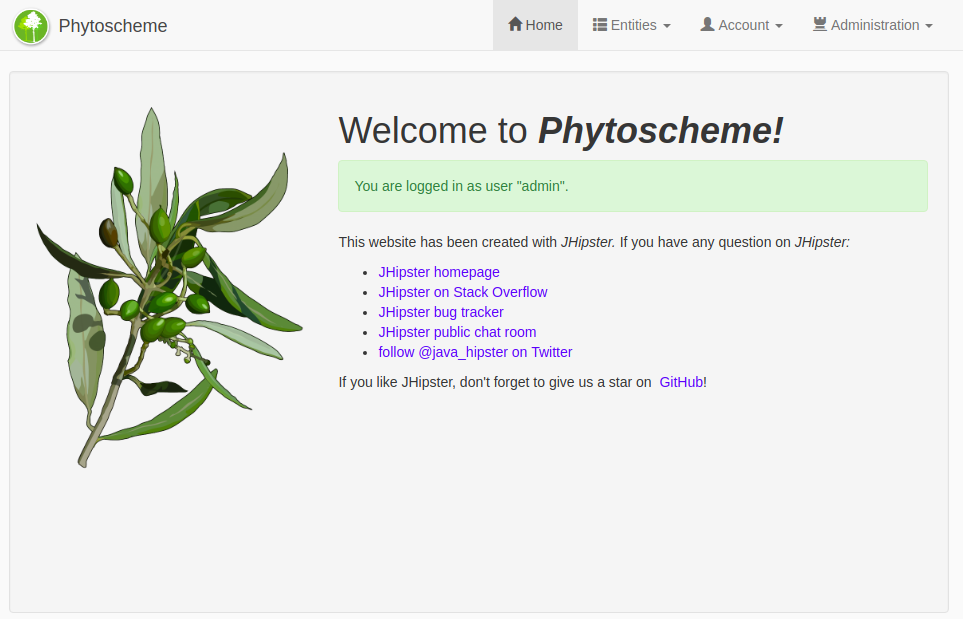
\includegraphics[width=\textwidth,height=\textheight,keepaspectratio]{Imagenes/Captura1}
    \caption{Captura de pantalla de la página de inicio de la aplicación \textit{Phytoscheme}.}
    \label{fig:capturaInicio}
\end{figure}

\par
\begin{figure}[!h]
    \centering
    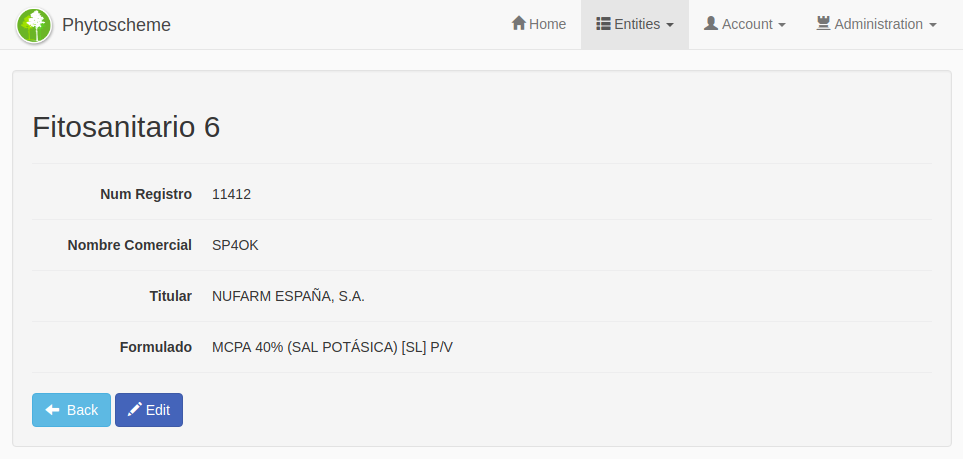
\includegraphics[width=\textwidth,height=\textheight,keepaspectratio]{Imagenes/Captura4}
    \caption{Captura de pantalla de la información de un producto fitosanitario.}
    \label{fig:capturaFitoDetalle}
\end{figure}


\par
\begin{figure}[!h]
    \centering
    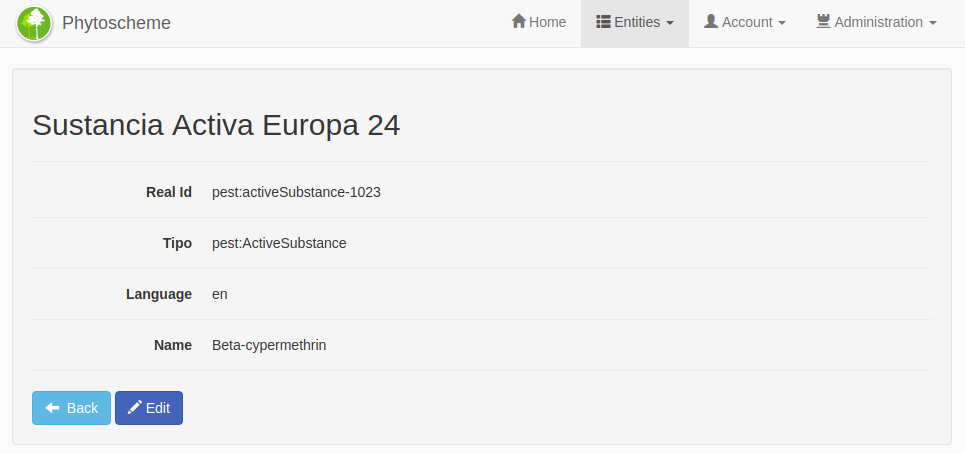
\includegraphics[width=\textwidth,height=\textheight,keepaspectratio]{Imagenes/Captura5}
    \caption{Captura de pantalla de la información de una sustancia activa.}
    \label{fig:capturaSustActDetalle}
\end{figure}
\chapter{Gestión} \label{d.gestion}
\section{Cálculo del coste de la hora de trabajo del alumno} \label{d.gestion.estimacion}
A continuación se exponen los cálculos desglosados y en detalle para calcular el coste de la hora de trabajo del alumno. Para conseguir el precio por hora para un salario de 1,500€ hacemos lo siguiente:
\begin{enumerate}
\item Calculamos el salario bruto anual:

Salario mensual × 12 meses

1,500.00 × 12 = \textbf{18,000€}
\item Hallamos el precio básico por hora:

Salario anual ÷ 2,080 horas posibles (8 horas × 5 días × 52 semanas)

18,000.00 ÷ 2,080 = \textbf{8.65€}
\item Sumamos el precio de las horas que no trabajarás:

14 días festivos × 8 hs. = 112 hs. +

21 días de vacaciones × 8 = 168 hs. +

7 días de incapacidad × 8 hs. = 56 hs.

\textbf{336 hs. × 8.65 de coste básico = 2,907.69€}
\item Calculamos el valor del tiempo que dedicas a presupuestos, reuniones, venta, formación... (tiempo administrativo):

50\% (2,080 hs. posibles - 336 horas que no trabajarás) × 8.65 coste básico.

\textbf{50\% × 1,744 hs. × 8.65 = 7,546.15€}
\item Calculamos el total de tus gastos fijos:

Alquiler mensual: 100.00 +

Servicios mensuales: 50.00 +

Autónomos mensual: 260.00 +

Otros gastos fijos mensuales: 50.00

Gastos fijos mensuales 460.00 × 12 meses = \textbf{5,520€ fijos anuales}
\item Sumamos el valor de las horas que no trabajas más el valor del tiempo de administración y el de los gastos fijos para obtener el precio extra anual por tu trabajo.

2,907.69 + 7,546.15 + 5,520.00 = \textbf{15,973.85€ de precio extra anual}
\item Ahora calculamos lo que ganarás al año:

2,080 hs. posibles al año - 336 hs. de vacaciones, festivos e incapacidad - 872 hs. de reuniones y presupuestos × 8.65 coste básico

\textbf{872 horas de trabajo × 8.65 = 7,546.15€ de beneficio anual.}
\item Calculamos el porcentaje de rentabilidad dividiendo el coste entre el beneficio:

15,973.85 ÷ 7,546.15 = 211.682\%

\item Por último para calcular la hora de trabajo sumamos el porcentaje de rentabilidad y el porcentaje de beneficio deseado a nuestro precio básico:

8.65 + 8.65 × 211.682\% + 8.65 × 20\% = \textbf{28.70€ por hora de trabajo}.
\end{enumerate}


















%%%%%%%%%%%%%%%%%%%%%%%%%%%%%%%%%%%%%%%%%%%%%%%%%%%%%%%%%%%%%%%%%%%%%%%%%%%%%%%%%%%


		\end{document}